\documentclass[UTF8,12pt,a4paper]{ctexart}

\usepackage[final]{pdfpages}
\usepackage{fancyhdr}
\usepackage{lastpage}
\usepackage{xcolor}
\usepackage{cite}
\usepackage{graphicx}
\usepackage{pifont}
\usepackage{float}
\usepackage{amsmath}
\usepackage{longtable}

\usepackage{url}
\usepackage{listings}
\usepackage[hidelinks]{hyperref}
\numberwithin{figure}{section}
\makeatletter
\def\UrlAlphabet{%
      \do\a\do\b\do\c\do\d\do\e\do\f\do\g\do\h\do\i\do\j%
      \do\k\do\l\do\m\do\n\do\o\do\p\do\q\do\r\do\s\do\t%
      \do\u\do\v\do\w\do\x\do\y\do\z\do\A\do\B\do\C\do\D%
      \do\E\do\F\do\G\do\H\do\I\do\J\do\K\do\L\do\M\do\N%
      \do\O\do\P\do\Q\do\R\do\S\do\T\do\U\do\V\do\W\do\X%
      \do\Y\do\Z}
\def\UrlDigits{\do\1\do\2\do\3\do\4\do\5\do\6\do\7\do\8\do\9\do\0}
\g@addto@macro{\UrlBreaks}{\UrlOrds}
\g@addto@macro{\UrlBreaks}{\UrlAlphabet}
\g@addto@macro{\UrlBreaks}{\UrlDigits}
\makeatother
\fancypagestyle{emptyStyle}
{
    \fancyhf{}
}
\fancypagestyle{abstractStyle}
{
    \fancyhf{}
    \fancyfoot[C]{\textcolor[gray]{0.6}{第\thepage 页~共\pageref{LastPage}页}}
    \renewcommand{\headrulewidth}{0pt}
    \renewcommand{\footrulewidth}{0pt}
}
\fancypagestyle{articleStyle}
{
    \fancyhf{}
    \fancyhead[L]{\ifodd\value{page}\textcolor[gray]{0.6}{\leftmark}\else\fi}
    \fancyhead[R]{\ifodd\value{page}\else\textcolor[gray]{0.6}{\rightmark}\fi}
    \fancyfoot[C]{\textcolor[gray]{0.6}{第\thepage 页~共\pageref{LastPage}页}}
    \renewcommand{\headrulewidth}{0pt}
    \renewcommand{\footrulewidth}{0pt}
}
\fancypagestyle{refStyle}
{
    \fancyhf{}
    \fancyhead[L]{\textcolor[gray]{0.6}{\leftmark}}
    \fancyfoot[C]{\textcolor[gray]{0.6}{第\thepage 页~共\pageref{LastPage}页}}
    \renewcommand{\headrulewidth}{0pt}
    \renewcommand{\footrulewidth}{0pt}
}
\setCJKmainfont{SimSun}[AutoFakeBold,AutoFakeSlant]
\setmainfont{TeX Gyre Termes}
\linespread{1.5}
\setcounter{tocdepth}{3}
\setcounter{secnumdepth}{5}
\ctexset {
section = {
name = {第,章},
number = \chinese{section},
break=\clearpage,
},
subsection = {
name = {第,节},
number = \chinese{subsection},
},
subsubsection = {
name = {第,小节},
number = \chinese{subsubsection},
},
paragraph={
name = {(,)},
number = \chinese{paragraph},
runin = false,
hang = true,
},
subparagraph={
name = {,.},
number = \Roman{subparagraph},
runin = false,
hang = true,
},
}

\date{}


\title{\Huge\textbf{2023年全国大学生信息安全竞赛\\作品报告}}

\begin{document}
\definecolor{mygreen}{rgb}{0,0.6,0}
\definecolor{mygray}{rgb}{0.5,0.5,0.5}
\definecolor{mymauve}{rgb}{0.58,0,0.82}
\lstset{
    backgroundcolor=\color{lightgray},
    basicstyle = \footnotesize,
    breakatwhitespace = false,
    breaklines = true,
    captionpos = b,
    commentstyle = \color{mygreen}\bfseries,
    extendedchars = false,
    frame =shadowbox,
    framerule=0.5pt,
    keepspaces=true,
    keywordstyle=\color{blue}\bfseries, % keyword style
    language = C++,                     % the language of code
    otherkeywords={string},
    numbers=left,
    numbersep=5pt,
    numberstyle=\tiny\color{mygray},
    rulecolor=\color{black},
    showspaces=false,
    showstringspaces=false,
    showtabs=false,
    stepnumber=1,
    stringstyle=\color{mymauve},        % string literal style
    tabsize=2,
    title=\lstname,
    escapeinside={@}{@},
    texcl=true,
}

\maketitle
\thispagestyle{empty}
\pagestyle{emptyStyle}
\vspace{6cm}
{
    \Large\textbf{作品名称}:\textbf{\underline{\makebox[10cm]{基于TrustZone-M函数级内存地址}}}
    
    \textbf{\underline{\makebox[13cm]{空间随机化的可信实时系统}}}
    
    \textbf{电子邮箱}:\underline{\makebox[10cm]{\textbf{213211377@seu.edu.cn}}}
    
    \textbf{提交时间}:\underline{\makebox[10cm]{\textbf{\today}}}
}
\clearpage
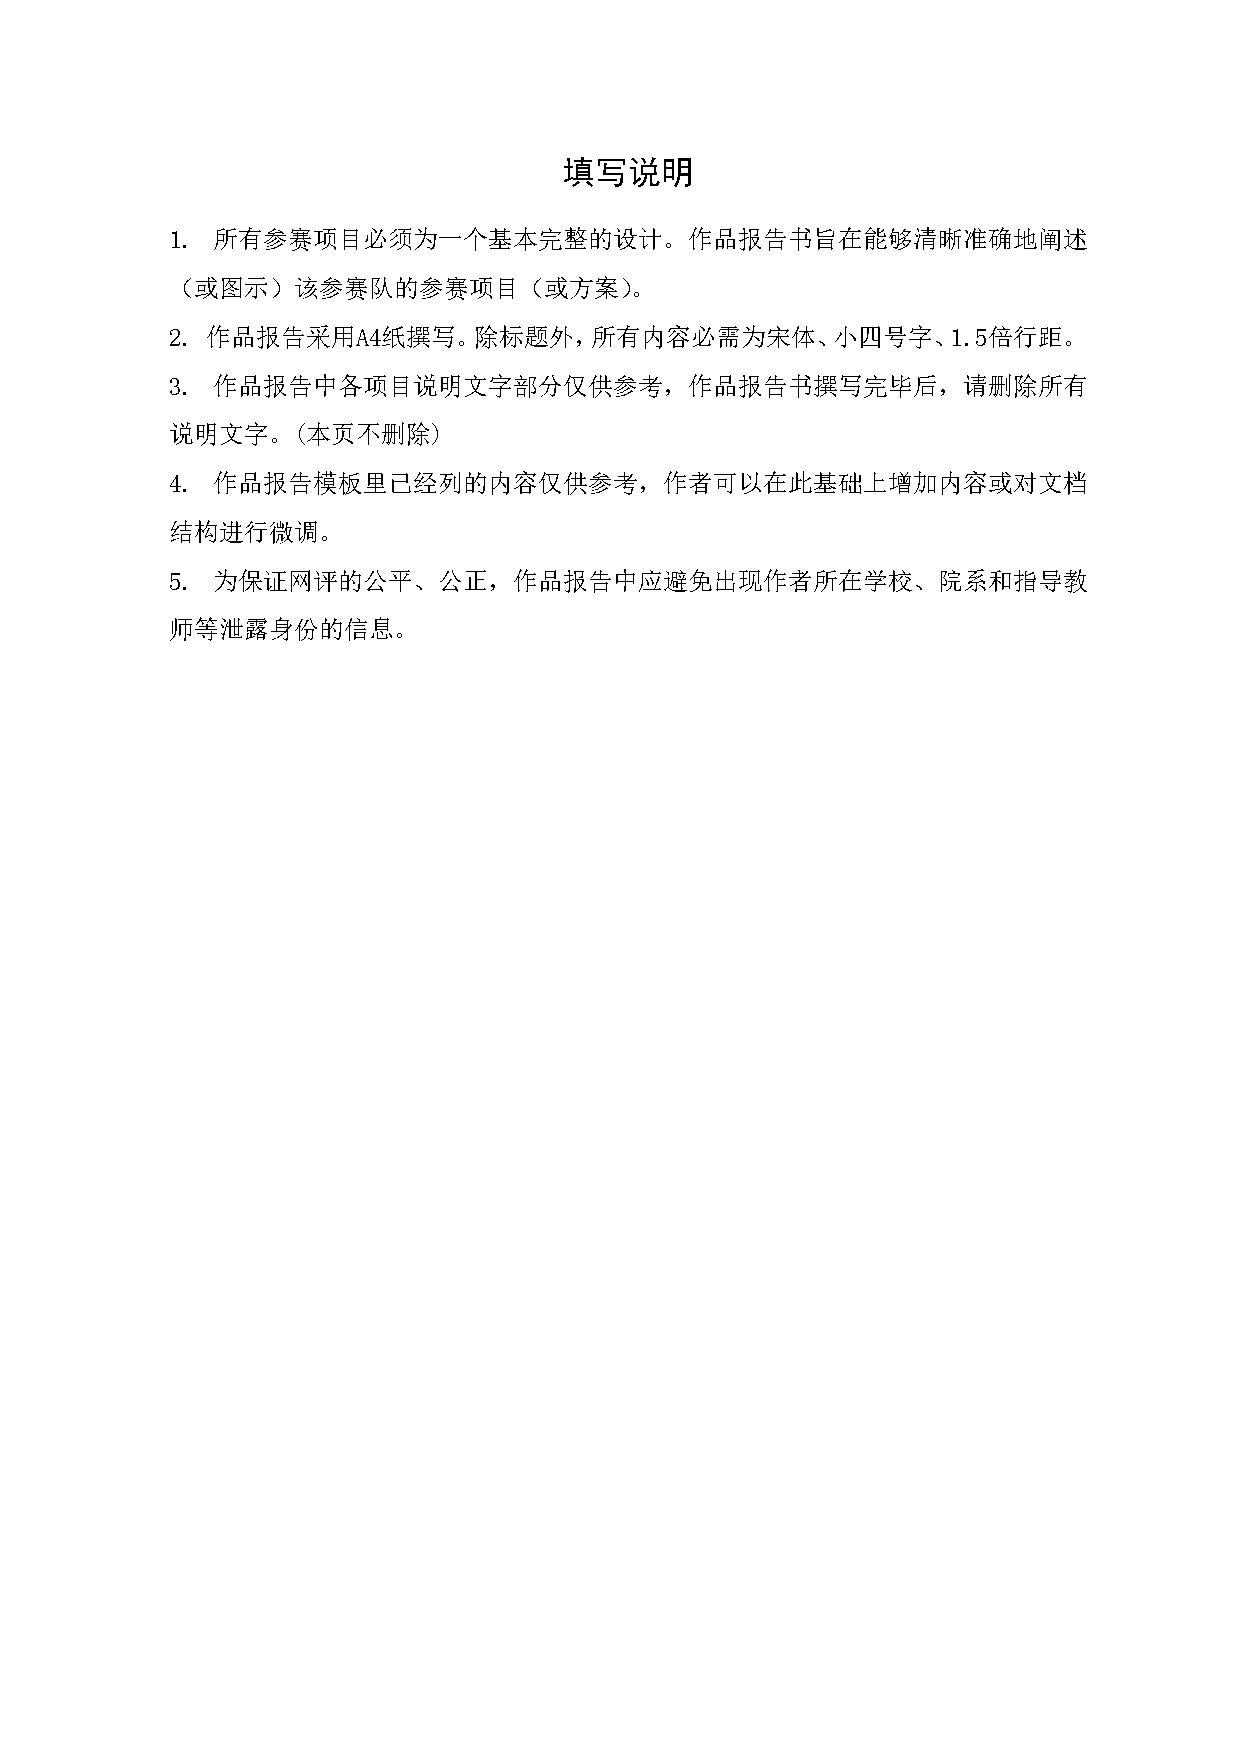
\includepdf{src/request.pdf}
\clearpage
\tableofcontents
\clearpage
\pagestyle{abstractStyle}
\setcounter{page}{1}
\section*{摘要}
\addcontentsline{toc}{section}{摘要}
\par 截至2023年,互联网物联网(IoT)设备面临严重的安全挑战。市场研究机构IoT Analytics发布了报告显示,2022年全球物联网连接数增长了18\%,达到143亿。分析预计,到2027年,全球联网物联网设备的数量将再增长至290亿。这些设备的安全性对人们的日常生活至关重要,涵盖智能可穿戴设备、家用电器、汽车、建筑警报系统和工业机械等各个领域。然而,很大一部分物联网设备是基于资源有限的微控制器实现的低端嵌入式系统,由于硬件资源不足、计算能力受限等特点,这些设备极易受到内存破坏引起的安全威胁。因此,近年来对维护其安全性的关注日益增加。

\par 基于微控制器的低端嵌入式系统通常运行裸机程序或实时操作系统,缺乏统一的可信软件来提供内存破坏的安全防御机制。在各种内存破坏引起的安全威胁中,面向返回编程(ROP)攻击是一种常见且具有广泛危害的攻击方式,它通过更改控制流来获取目标设备的控制权。然而,由于基于微控制器的低端嵌入式系统对低成本和低功耗的要求,现有的通用防御机制难以直接部署,这给防御内存破坏攻击带来了巨大挑战。

\par 针对这一日益严峻的安全问题,本作品利用地址空间布局随机化技术和ARM TrustZone可信执行环境构建技术,针对基于微控制器的低端嵌入式系统的有限计算和内存资源,设计并实现了一个完整的可信执行环境和函数级地址空间布局动态随机化机制。该机制有效地防御了针对系统和内存的破坏攻击,并为嵌入式系统设备提供了安全可靠的服务。该技术已成功部署在实时操作系统FreeRTOS和可信执行环境Trusted Firmware-M上,使得应用程序能够在开源实时操作系统的调度下运行并进行函数级的地址空间布局随机化,兼顾了嵌入式系统设备的实时性要求和安全性要求。

\par 本作品的基本框架是基于主流实时操作系统FreeRTOS和面向ARM低端嵌入式系统的可信执行环境Trusted Firmware-M。FreeRTOS提供多任务调度以满足嵌入式系统的实时需求,而Trusted Firmware-M旨在提供一个可配置和可裁剪的安全固件平台,支持从小型嵌入式设备到高端安全系统的多种应用场景。本作品对Trusted Firmware-M进行了针对性的裁剪和部署,使其更适用于嵌入式设备,并添加了自定义的安全分区,以适应更多的应用场景和潜在的安全威胁。在Trusted Firmware-M的安全分区服务中,本作品实现了函数级地址空间布局动态随机化服务,为非安全区提供实时安全的函数级地址空间布局随机化,有效防御了ROP攻击。此外,本作品还对随机化过程进行了性能和内存优化,使其更适用于广泛的嵌入式设备。

\par 此外,本作品还使用STM32L562E-DK开发板实现了一套嵌入式系统应用并将本作品技术进行部署,并且在此基础上针对ROP攻击的安全性和地址空间布局随机化的性能进行了详细的测试和分析,验证了本作品的可行性和有效性。
\clearpage
\pagestyle{articleStyle}
\section{作品概述}
\subsection{作品背景}
\par 近年来,伴随着信息技术的飞速发展,以智能家居、智慧交通、智慧医疗等为应用场景的物联网产业得到了迅猛发展。与此同时,物联网设备的数量也在飞速增长。到2020年底,全球物联网设备连接,如联网的汽车、智能家居设备、联网的工业设备等,数量达到了117亿,约占全球的54\%,首次超过了非物联网设备连接,如智能手机、笔记本电脑和计算机等。作为全球最大的物联网市场,中国在这一领域更是处于领先地位。到目前为止,已投入使用的物联网设备数量已经超过了144亿,预计到2025年物联网设备数量将达到270亿\cite{StateOfIOT}。
\par 虽然物联网的发展已渐成规模,但其安全问题也越来越突出。从物联网设备的角度来看,很多物联网设备是基于微控制器(Micro Controller Unit,MCU)实现的嵌入式系统,比如车载控制设备、智能锁具、无人机、可植入医疗设备等。与通用系统一样,由于嵌入式系统硬件设计不当或软件开发不当,使运行在嵌入式系统上的软件通常存在不同类型的安全漏洞,进而引发一系列的安全问题。自从2017年以来,上百个嵌入式系统的安全漏洞已经在NVD平台上被披露出来,对设备安全和用户隐私造成了严重影响。例如,谷歌Project Zero团队发现部分手机搭载的WiFi模块漏洞对用户手机造成安全威胁\cite{beniamini2017project};家庭安防产品Ring被曝出存在可以让攻击者监控用户家庭的安全漏洞等\cite{Amazon}。随着嵌入式系统安全的重要性不断提高,维护嵌入式系统的安全变得至关重要。
\par 深入研究嵌入式系统的安全威胁后发现,嵌入式系统的安全威胁很大一部分来自二进制的内存破坏攻击,主要包括代码破坏攻击(Code Corruption Attack),控制流劫持攻击(Control-flow Hijack Attack),面向数据的攻击(Data-only Attack)以及信息泄露攻击(Information Leak Attack)\cite{clements2017protecting,papp2015embedded}。其中控制流劫持攻击最为常见,例如ROP攻击等。ROP攻击是利用程序空间已有指令序列,通过覆盖栈上的函数返回地址串联起一系列的gadgets(一段以返回指令结尾的代码段),将程序控制流转向攻击程序流的攻击方法。在通用系统中\cite{cowan1998stackguard,angelfire,tanenbaum1997operating,bojinov2011address,backes2014you},已有许多防御机制被部署以防御ROP攻击,如DEP(Data Executable Prevention),栈保护机制,代码多样化(Code Diversification),地址空间布局随机化(Address Space Layout Randomlization,ASLR),内存只可执行(Execute Only Memory,XOM),指令集随机化(Instruction Set Randomization,ISR)等。现有针对控制流劫持攻击的防御中,主要以控制流完整性保护技术以及地址空间信息隐藏技术最具代表性。但c由于嵌入式系统其低功耗、低成本的的要求,其硬件资源受到了很大的限制,导致在通用系统中的防御机制无法直接部署,尤其是基于8位,16位,32位微控制器的嵌入式系统\cite{PositionPaper}。这些低端嵌入式系统大多处理器工作频率在100MHz以下,在存储上只有几百KB的Flash以及几十KB的RAM,并且它们普遍不支持内存管理单元(Memory Management Unit,MMU)\cite{abbasi2019challenges,almakhdhub2020mu}。同时,运行在这些设备中的嵌入式系统软件一般用 C/C++语言编写实现,因此,与通用系统一样,这些嵌入式系统软件易受到内存破坏攻击,进而引发一系列的安全问题\cite{roemer2012return},例如攻击者可以利用内存破坏漏洞来向受攻击的应用程序中注入恶意代码,从而导致代码执行漏洞。这种攻击可能会让攻击者控制设备、窃取数据或对系统进行其他恶意行为。除此之外,还可能产生拒绝服务攻击,系统提权,数据泄露等一些列安全问题。因此,现有的内存破坏防御机制无法直接应用于低端嵌入式系统,而低端嵌入式系统尚缺乏有效的内存破坏防御机制,使其安全性受到严重威胁。
\par 一般来说,可信执行环境由可信执行环境操作系统(Trusted Execution Environment Operating System,TEE OS)以及安全服务(或称为TA,Trusted Application)构成,可信执行环境操作系统主要为用户调用安全服务提供安全的通信机制。为了满足嵌入式系统对安全日益增长的需求,ARM在2015年提出了面向Cortex-M系列芯片的TrustZone-M技术\cite{armv8mARM,ARMv8-MATO},TrustZone-M技术将嵌入式系统软硬件等资源分为安全世界和非安全世界,安全世界可以直接访问非安全世界资源,但非安全世界不能直接访 问安全资源,其对安全世界资源的访问需要通过安全世界提供的 API。这些 API 实现了身份验证,确保安全世界资源被正确使用。严格控制非安全世界与安全世界间的访问,旨在为系统提供一个TEEOS。由于其具有灵活性,易于开发,低功耗等优势,在移动终端领域,ARM公司针对Cortex-A系列芯片提出的TrustZone技术已经在大多数智能手机上得到TEEOS的配备,例如高通实现的QSEE,华为实现的TEEOS,三星实现的Knox等,该技术主要被用来提供安全支付,指纹服务,文件保密等安全服务。但是在低端嵌入式领域,目前基于TrustZone-M技术提供TEEOS的研究较少,其中较为流行的有两个,一个是ARM公司主导的开源作品Trusted Firmware-M(TF-M),另一个是Trustonic公司研发的闭源作品Knibi-M\cite{ARMv8-MATO},前者虽然开源但对实时操作系统的兼容性较差,后者不开源且目前仅支持Microchip下的SAML11系列SoC(Systemon Chip),两者都可为用户提供多种安全服务,如安全加密,安全密钥管理等,但都未提供对控制流劫持攻击的安全保护机制。
\par 目前,有三个主要方向用于提高低端嵌入式系统的安全性:首先是利用低端嵌入式系统的硬件设施,例如采用前文提到的ARMv8-M 架构下的TrustZone-M 技术、系统调试单元和内存保护单元(Memory Protection Unit,MPU)等,实现内存隔离、内存检测和访问控制等安全防护措施。然而,由于嵌入式系统硬件的多样性,这要求系统开发者针对不同硬件环境实现相应的安全机制,导致可扩展性较差。此外,还需额外的硬件支持,从而增加成本和工程开销。第二个方向是利用编译器技术,在对代码进行词法和语法分析后,在重新编译现有嵌入式系统源码的过程中加入额外代码以实现特定的防御机制,从而提高系统安全性。例如,采用软件错误隔离(Software Fault Isolation,SFI)技术实现代码块隔离,利用代码多样化(Code Diversification)技术抵御代码复用攻击等。这种方法的优点是无需更改原有系统的软硬件,避免了成本和工程开发上的额外开销。但是,由于编译器在软件层面提高系统安全性,因此可能会给代码的执行效率和性能带来额外负担。最后一个方向是综合前两者,通常针对已有可信硬件的低端嵌入式系统。在编译过程中加强代码安全性,并将支持可信硬件的防御机制代码直接编译至目标代码,具有较好的可扩展性。由于此类方法本质上仍然基于编译器对代码进行重新编译,因此对系统开发具有较好的透明性。同时,得益于可信硬件的支持,对嵌入式系统的安全性以及性能也有较好的兼顾。
\par 虽然已经出现了众多的安全防护技术,如StackGuard阻止栈溢出、DEP阻止代码注入等,但是每个技术只能防御某一种特定方式的攻击,要将这些技术集成在一起实现困难且开销大,而新的攻击方式还在不断出现,为了解决这些不足,研究人员提出了从另一个角度对系统进行保护的安全技术,即地址空间布局随机化(Address Space Layout Randomization,ASLR),ASLR是一种通用计算机系统安全技术,在进程的地址空间中随机放置可执行文件、库、堆和栈的基地址位置。由ASLR执行内存地址的随机布局后,攻击者不再知道所需代码片段(例如函数或ROP gadgets)实际地址,使攻击难度大大增加。ASLR不会从系统中彻底清除漏洞,而是使攻击者利用现有漏洞更加艰巨。ASLR由PaxProject在2001年作为Linux修补程序创建,实现方法是在进程加载时,对栈基地址的4-27位共24位进行随机;对包括主程序映像、静态数据区、堆这一连续区域的基地址12-27位共16位进行随机;对共享加载库地址的12-27位共16位进行随机。ASLR技术加上数据保护执行DEP构成了一个完整的系统防护方案,DEP技术迫使攻击者使用空间中现有代码,ASLR使得这些空间中现有代码地址不可确定,由此能大大降低攻击成功的概率,在当时Linux系统中得到广泛应用。并于2007年从Vista开始集成到Windows操作系统中。之后相继出现在各种主流通用操作系统中。虽然,目前针对内存破坏攻击的运行时防御机制已广泛部署在通用系统,但这些防御机制往往需要硬件支持以减少其所引入的性能开销,比如MMU\cite{abbasi2019challenges,almakhdhub2020mu}等。然而,嵌入式系统由于其低功耗、低成本的的要求,使其硬件资源受到了很大的限制,ASLR技术难以实施。
\par 因此,为保护物联网设备系统的安全,本作品针对目前控制流劫持攻击对低端嵌入式系统的威胁日益增大,缺乏有效的控制流劫持防御机制,且ASLR技术在嵌入式系统中难以实施的问题,对低端嵌入式系统的控制流劫持攻击设计实现了基于ARM TrustZone-M的函数级动态随机加载技术,该技术对整个代码空间进行随机化,包括用户程序以及实时操作系统内核,并且支持当下流行的可信执行环境操作系统Trusted Firmware,构成了整个系统原型。
\par 首先,本作品自主设计实现了基于TrustZone-M的可信执行环境操作系统,为非安全世界提供实时可信的安全服务。先为在非安全世界调用安全服务时保护安全世界间的数据通信安全,并保证其请求资源的合法性,设计安全/非安全世界的安全通信机制。同时,借助TF-M,为非安全世界提供可靠的安全服务。然后,为实现对安全服务的多任务并发调用,需要保证安全服务在非安全世界产生任务切换后依然可以恢复执行并且能将响应结果通过安全内核返回至原非安全世界任务。现有实时操作系统(如FreeRTOS)已支持任务在安全世界调用安全函数,并且可以在任务切换后恢复安全函数的执行。具体地,在切换至某一就绪任务时,非安全世界的任务调度器会检查其之前调用的安全函数是否未执行完,若存在,则会先恢复该任务所对应的安全函数并执行,然后将响应结果以函数返回的方式直接返回给该任务。这种方式虽然可以实现多任务对安全函数的并发调用,但是由于是任务直接调用安全函数,一旦安全函数存在漏洞则会破坏整个安全世界的安全性。本作品基于FreeRTOS设计了安全服务多任务并发调用技术。
\par 其次,在基于TrustZone-M可信执行环境的基础上,重点研究系统运行时低端嵌入式系统上部署地址空间布局随机化(ASLR)技术以实现对控制流劫持攻击的防御。为保证运行时系统代码地址空间布局随机化,本作品提出一种基于MPU的函数级地址空间布局随机化技术FASLR,实现系统运行时函数级的地址空间布局随机化。该技术首先设计静态信息提取技术以对系统以及函数信息进行收集与管理,实现函数运行时的实时状态感知。随后设计基于MPU的函数动态加载机制以对系统进行函数级地址空间布局动态随机化,实现对函数运行时代码地址空间布局信息的实时隐藏,最后设计函数级随机化内存管理机制,实现高利用率、高性能的函数随机加载内存管理。

\par 因此,本作品在抵抗控制流劫持攻击对低端嵌入式系统的威胁等方面具有重要的研究价值和实践意义。


\subsection{研究现状}
\par 随着ARMv8-M架构设备在物联网市场的普及,低端嵌入式系统的安全性已成为一个受到广泛关注的问题。ROP攻击、缓冲区溢出、格式化字符串漏洞等攻击为低端嵌入式系统带来了严重的内存破坏安全威胁。为应对现有安全防护技术通用性较差的挑战,研究人员提出了一系列内存破坏防御技术,其中,ASLR地址空间布局随机化技术从不同的角度、更细的粒度对系统进行保护。此外,为了提高低端嵌入式设备的安全性,现有的研究还探索了基于TrustZone-M技术的可信执行环境构建技术,该技术旨在通过安全的通信机制为用户应用程序提供可信软件服务。此外,Trusted firmware-M开源固件作品提供了一个全面的安全框架,用于保护Arm Cortex-M设备的安全性。

\subsubsection{面向低端嵌入式系统的内存破坏安全威胁}
\paragraph{ROP(Return Oriented Programming) 面向返回编程技术}
\subparagraph{ROP基本原理}
\par 面向返回编程(Return Oriented Programming,ROP)是一种典型的基于代码复用技术的攻击,它在计算机系统的安全领域引起了广泛的关注和研究。ROP攻击的核心思想是利用程序或动态加载库中已存在的汇编代码片段,称为gadgets,来构建恶意代码执行流。攻击者通过覆盖栈的返回地址以及后续地址空间,将这些gadgets连接在一起,形成一个恶意代码执行链,从而改变程序的正常执行流程。
\par 在ROP攻击中,关键的一步是找到满足攻击条件的gadgets以及它们的地址。这些gadgets是程序中常见的指令序列,例如加载寄存器、执行函数调用和跳转等。攻击者需要通过精心的分析和探测,找到可用于构建ROP链的合适gadgets,并确定它们在内存中的地址。
\par 如图\ref{ROP}所示,具体攻击步骤如下:
\begin{itemize}
    \item[(1)] 带有栈溢出漏洞的程序开始执行,用户输入数据到返回地址处,并将返回地址覆盖为代码段中原有的代码片段地址 return address 1,继续向后覆盖 return address 2、return address 3 等;
    \item[(2)] 当前函数执行结束,程序流寄存器从返回地址处取得下一条指令地址,此时返回地址的内容为 ret address 1,程序流跑到 gadget1 执行;
    \item[(4)] gadget1 执行完毕后,程序执行 ret 指令,从栈顶取得下一条指令地址,也就是 return address 2,程序流跑到 gadget 2 执行;
    \item[(5)] gadget 2 执行完毕后,程序执行 ret 指令,从栈顶取得下一条指令地址,也就是 return address 3,程序流跑到 gadget 3 执行;
\end{itemize}

\begin{figure}
    \centering
    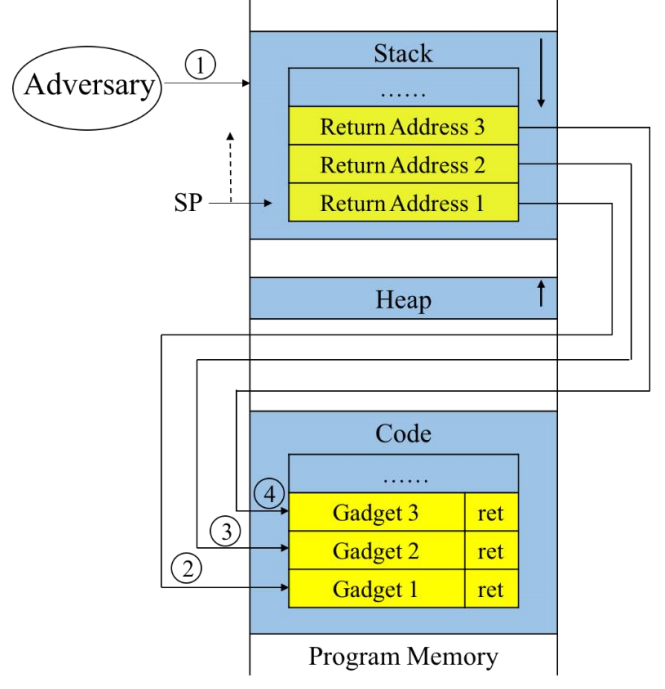
\includegraphics[scale=0.35]{graph/ROP.png}
    \caption{ROP攻击流程}
    \label{ROP}
\end{figure}
综上所述,攻击者进行攻击后会使得程序执行流变为gadget1->gadget2->gadget3。

\par 为了有效实施ROP攻击,攻击者需要克服一些技术挑战。首先,他们需要了解目标程序的内存布局,包括栈的结构、函数调用和返回的机制等。其次,攻击者需要能够识别和利用程序中的漏洞,例如堆栈溢出或格式化字符串漏洞,以覆盖返回地址并控制执行流程。此外,攻击者还需要解决ROP链的构建问题,确保gadgets的执行顺序和参数传递正确,以实现所需的恶意操作。

\subparagraph{ROP研究现状}
ROP攻击的研究现状主要包括以下几个方面:\\
\textbf{i. 漏洞利用}
\par ROP攻击最初是在针对堆栈溢出和格式化字符串等常见漏洞的利用中出现的。堆栈溢出漏洞是指当程序在处理输入数据时,将数据写入到栈空间中的缓冲区时,超出了缓冲区的边界。攻击者可以利用这个漏洞覆盖栈上的返回地址,并将其指向gadgets序列,从而控制程序的执行流程。
\par 研究人员在漏洞利用方面做了大量的工作,探索和利用各种漏洞形式。例如,通过输入数据中的特定格式化字符串,攻击者可以覆盖函数的返回地址,从而改变程序的执行流程。另一个常见的漏洞是缓冲区溢出,攻击者可以将恶意数据输入到缓冲区中,覆盖返回地址并控制程序的执行。
\par 为了成功利用漏洞进行ROP攻击,研究人员使用了多种技术和方法。他们通过分析程序的源代码、二进制代码和运行时行为,寻找潜在的漏洞点。然后,他们通过构造适当的输入数据,精确地控制溢出和覆盖返回地址,使其指向gadgets序列的开头。
\par 此外,研究人员还致力于发现新的漏洞形式和利用方法。他们通过不断深入研究和漏洞挖掘,提高对程序漏洞的理解,并开发出新的技术来克服现有防御机制。\\

\textbf{ii. ROP链的构建}
\par 构建有效的ROP链需要解决多个技术挑战,包括gadgets的选择、ROP链的布局和参数的传递等。
\par 首先,研究人员提出了各种技术和工具来发现和选择合适的gadgets。其中,静态分析是一种常见的方法,通过对目标程序的二进制代码进行分析,提取出符合特定要求的gadgets。这种方法可以利用静态代码分析工具来自动化地识别和提取gadgets,大大减少了手动分析的工作量。此外,动态分析技术也被广泛应用于ROP链的构建中。通过在运行时观察程序的行为并收集执行信息,可以动态地发现和提取gadgets,从而构建有效的ROP链。
\par 其次,研究人员关注ROP链的布局和连接方式。由于gadgets是以返回指令结尾的代码片段,因此它们需要按照正确的顺序连接在一起,以实现所需的操作。研究人员提出了多种布局策略,例如线性布局和分支布局。线性布局将gadgets按照顺序连接,每个gadget的返回地址即为下一个gadget的地址,这种布局简单直观。而分支布局则通过跳转指令来实现gadgets的连接,可以更灵活地构建ROP链。
\par 此外,参数的传递也是ROP链构建的关键问题。由于ROP攻击的目的是改变程序的执行流程,因此需要能够控制寄存器的值或者传递特定的参数。研究人员通过分析目标程序的调用约定和参数传递方式,设计了各种技术来在ROP链中传递参数。这些技术包括将参数值存储在已知地址上、利用栈上的数据结构传递参数,或者通过其他寄存器来传递参数等。
\par 为了自动化和简化ROP链的构建过程,研究人员还提出了一些工具和框架。这些工具可以根据目标程序的特征和需求,自动生成合适的ROP链。它们通常结合静态分析和动态分析技术,提供了便捷的方式来发现gadgets、构建ROP链和验证攻击效果。\\

\textbf{iii. ROP攻击的通用性}
\par 最初的ROP攻击是针对特定的漏洞和特定的程序实现的,但随着研究的深入,人们逐渐认识到ROP攻击具有广泛的适用性,并可以用于绕过各种内存保护机制和操作系统的安全措施。
\par 研究人员发现,由于现代计算机体系结构中的代码复用现象普遍存在,攻击者可以通过组合已有的代码片段(gadgets)来构建任意的恶意操作序列。这些gadgets可以来自于程序本身、动态链接库(DLL)或操作系统中的代码段,因此攻击者并不需要直接注入恶意代码,而是利用现有的代码片段来构造攻击载荷。这使得ROP攻击具有很强的灵活性和适应性。
\par ROP攻击的通用性研究主要集中在以下几个方面:
\begin{itemize}
    \item 研究不同平台和体系结构下的ROP攻击:研究人员对不同的计算机平台和体系结构进行了广泛的研究,包括x86、ARM、MIPS等。他们研究了各种指令集下的gadgets提取和ROP链构建技术,以及不同平台下的ROP攻击的实际可行性和效果。
    \item 绕过内存保护机制和安全措施:ROP攻击具有绕过许多现有的内存保护机制和安全措施的能力,如地址空间布局随机化(ASLR)、数据执行保护(DEP)和栈保护技术等。研究人员致力于研究和发展新的技术和方法,以提高对抗这些防御机制的能力。
    \item 跨平台和跨应用程序的ROP攻击:除了单个应用程序内的ROP攻击,研究人员还开始研究跨平台和跨应用程序的ROP攻击。他们发现,可以通过在不同的应用程序之间共享ROP链和gadgets,将攻击面扩展到更广泛的环境中,从而进一步提高攻击的成功率。
    \item 自动化ROP链的生成和分析:为了简化ROP攻击的构建过程,研究人员致力于开发自动化工具和技术,用于生成和分析ROP链。这些工具可以通过静态或动态分析程序的二进制代码,提取可用的gadgets,并自动生成有效的ROP链,从而减少攻击者的手动工作量。
\end{itemize}

\textbf{iv. 防御技术的研究}
\par 随着ROP攻击的不断演进和威胁的增加,研究人员和安全专家开始致力于开发各种防御技术来减轻或阻止ROP攻击的影响。以下是一些主要的ROP防御技术:
\begin{itemize}
    \item 内存随机化(ASLR):内存随机化是一种常见的防御技术,通过随机化操作系统和应用程序的内存布局,使攻击者难以准确地确定gadgets和其他关键数据结构的位置。通过在每次系统启动时随机化内存布局,内存随机化增加了攻击者发现和利用ROP链所需的工作量。
    \item 控制流完整性保护(CFI):控制流完整性保护技术旨在检测和阻止程序执行流程的异常跳转。CFI技术通过在程序中插入额外的检查代码来验证每个间接跳转的目标是否合法,从而防止攻击者利用ROP链来改变程序的执行流程。
    \item ROP检测:ROP检测技术旨在通过静态或动态分析程序的二进制代码来识别和检测ROP链的存在。这些技术通常基于对gadgets的模式匹配和特征分析,以及对程序执行流的监控和分析。
    \item 代码执行完整性(Code-Reuse Integrity):代码执行完整性技术试图保护程序的代码区域,以防止攻击者通过覆盖和篡改代码来构建ROP链。这些技术可以使用硬件支持或软件实现,例如通过保护指令流完整性和校验代码签名等方式。
    \item 随机化ROP链(Randomizing ROP Chains):这项技术旨在增加攻击者构建有效ROP链的难度。通过在每个gadget之间插入无效指令或垃圾指令,使攻击者无法准确地构建有效的ROP链,从而降低攻击成功的概率。
    \item 硬件支持:一些硬件技术也可以用于增强系统的ROP防御能力。例如,通过硬件支持的内存隔离机制和可执行代码的只读存储器等技术,可以减少攻击者对内存数据的篡改和执行的可能性。
\end{itemize}

\paragraph{缓冲区溢出}
\par 缓冲区溢出(Buffer Overflow)是一种常见的安全漏洞,它的基本原理是在程序中的缓冲区中写入超出其容量的数据,导致多余的数据溢出到相邻的内存区域。
\par 在计算机程序中,缓冲区是用来存储数据的一块内存区域。缓冲区通常具有固定的大小,程序在使用缓冲区时需要确保写入的数据不会超过缓冲区的容量。然而,如果程序没有正确地检查和限制写入数据的大小,攻击者就可以通过构造恶意输入来触发缓冲区溢出\cite{lhee2003buffer}。
\par 攻击者通过向目标程序输入超出缓冲区容量的数据,将多余的数据写入到相邻的内存区域。这可能导致以下几种情况:
\begin{itemize}
    \item 覆盖关键数据:溢出的数据可能会覆盖其他重要的数据结构,如函数指针、返回地址、局部变量等。通过精心构造的输入数据,攻击者可以改变这些关键数据的内容,从而控制程序的执行流程。
    \item 破坏栈结构:在使用函数调用时,程序使用栈(stack)来存储函数的局部变量、函数参数和返回地址等信息。如果溢出的数据覆盖了栈中的这些数据,就会破坏栈的结构,导致程序无法正确地返回到调用函数的位置。
    \item 执行恶意代码:攻击者可以将溢出的数据中的一部分修改为指向攻击者精心构造的恶意代码的地址。当程序执行到被修改的函数指针或返回地址时,控制流将被劫持到攻击者的恶意代码,从而执行恶意操作。
\end{itemize}

\par 缓冲区溢出攻击通常利用了程序中对缓冲区的不正确处理,包括缺乏输入验证、缺乏边界检查、使用不安全的函数等。攻击者可以利用这些漏洞来覆盖关键数据并劫持程序的执行流程,从而实现未授权的访问、执行恶意代码、提升特权等恶意行为。
\par 攻击者利用缓冲区溢出漏洞可以实现以下几个步骤\cite{cowan2000buffer}:
\begin{itemize}
    \item[(1)] 寻找目标:攻击者首先需要找到一个存在缓冲区溢出漏洞的目标程序。通常,攻击者会选择具有网络功能或用户交互的应用程序,如网络服务器、操作系统服务、Web应用程序等。
    \item[(2)] 构造恶意数据:攻击者需要构造特定的输入数据,其中包含能够触发缓冲区溢出的数据。这通常包括长于目标缓冲区大小的输入数据,例如长字符串、大型文件或网络数据包。
    \item[(3)] 溢出触发:攻击者向目标程序发送构造的恶意数据,导致目标程序将数据写入超出缓冲区边界的内存区域。这可能覆盖其他重要的数据结构,如函数指针、返回地址、局部变量等。
    \item[(4)] 控制流劫持:由于溢出数据可能覆盖了函数指针或返回地址,攻击者可以将这些数据修改为指向攻击者精心构造的恶意代码的地址。当目标程序执行到被修改的函数指针或返回地址时,控制流将被劫持到攻击者的恶意代码。
    \item[(5)] 执行恶意代码:一旦控制流被劫持,攻击者的恶意代码将被执行。这可能包括执行远程命令、访问敏感数据、修改系统配置、传播恶意软件等恶意行为。
\end{itemize}

\paragraph{格式化字符串漏洞}
\par 格式化字符串漏洞(Format String Vulnerability)是一种常见的安全漏洞,其攻击原理是利用程序中对格式化字符串的不正确处理,导致攻击者可以读取或修改内存中的数据,执行未授权操作或者执行任意代码\cite{lhee2003buffer}。
\par 格式化字符串漏洞通常出现在使用格式化字符串函数(如printf、sprintf、fprintf等)时,当格式化字符串中的占位符与实际提供的参数不匹配时,就可能引发漏洞。
\par 格式化字符串漏洞的攻击步骤可以分为以下几个阶段:
\begin{itemize}
    \item[(1)] 构造恶意格式化字符串:攻击者需要构造一个恶意的格式化字符串,其中包含特殊的格式化占位符和参数。这些特殊的占位符用于读取或修改内存中的数据。
    \item[(2)] 传递恶意格式化字符串:攻击者需要将构造的恶意格式化字符串传递给目标程序。这可以通过用户输入、命令行参数、网络传输等方式完成。
    \item[(3)] 触发格式化字符串函数:目标程序在处理恶意格式化字符串时,会调用相应的格式化字符串函数(如printf、sprintf等)。这些函数会按照格式化字符串的指示,从栈或寄存器中读取相应的参数值。
    \item[(4)] 读取敏感数据:攻击者可以使用特殊的格式化占位符(如\%lx、\%s等)来读取栈中的敏感数据。通过逐个读取栈上的数据,攻击者可以获取函数的返回地址、局部变量的值等敏感信息。
    \item[(5)] 修改内存数据:攻击者可以使用特殊的格式化占位符(如\%n)来修改内存中的数据。通过合理构造格式化字符串,攻击者可以将指定的值写入任意内存地址,从而修改重要数据,如函数指针、全局变量等。
    \item[(6)] 控制流劫持:一旦攻击者成功修改了函数指针或返回地址,就可以将控制流劫持到攻击者控制的恶意代码。这使得攻击者能够执行任意代码,从而实现未授权的操作、特权提升或者远程命令执行等攻击行为。
\end{itemize}

\subsubsection{内存破坏防御技术}
\par 内存破坏问题一直是计算机安全领域研究的重点之一,它一般存在于C或者C++编写的软件中,内存破坏攻击都是通过触发一个内存错误以实现攻击,比如悬挂指针,数组越界访问等。根据Szekeres\cite{6547101}等人对内存破坏攻击的调研,攻击者可以利用内存破坏漏洞实现代码破坏攻击(Code Corruption Attack),控制流劫持攻击(Control-flow Hijack Attack),面向数据的攻击(Data-only Attack)以及信息泄露攻击(Information Leak Attack)。其中,尽管在低端嵌入式系统安全领域已存在些许安全机制以抵御不同类型的内存破坏攻击\cite{7958583,8806725,almakhdhub2020mu},然而,控制流劫持攻击依旧是该领域的主要威胁,现有针对控制流劫持攻击的防御中,主要以控制流完整性保护技术以及地址空间信息隐藏技术最具代表性。
\paragraph{控制流完整性保护技术}
\par 控制流完整性保护技术是指对控制流转移进行检查以防御控制流劫持攻击。控制流劫持攻击是由于内存安全问题所引起的针对间接控制流转移的篡改,目前可分为前向控制流转移攻击和后向控制流转移攻击。前向是指攻击者通过篡改函数指针或者虚函数表等来达到转移控制流的目的,而后向则是指通过篡改函数返回地址来改变控制流转移,因此控制流完整性保护可分为前向控制流完整性保护以及后向控制流完整性保护。由于前向控制流完整性保护性能很大一部分取决于CFI的目标集(即CFI所保护的间接跳转的集合)中产生调用的次数,而对于低端嵌入式系统来说,其代码量较少\cite{almakhdhub2020mu}导致其CFI目标集也相对较少,因此可以通过直接部署通用系统的前向完整性保护技术\cite{burow2017control}以保证前向控制流完整性。然而,对于基于返回地址的后向完整性保护来说,函数的返回地址由于其在程序中所占数量庞大,且更容易被攻击者所利用\cite{almakhdhub2020mu},因此后向完整性保护在低端嵌入式系统领域依然具有较大的挑战性。
\par Sun等人\cite{9152803}针对嵌入式系统提出了操作完整性(Operation Execution Integrity,OEI),并设计了一个端到端的系统OAT(OEI ATtester),该系统可在基于ARM的嵌入式设备上实现OEI的远程认证。OEI包括控制流完整性以及数据流完整性。在控制流完整性上,OAT利用远程证明机制来提高在嵌入式设备上的性能,它结合对控制流转移以及返回的跟踪,计算其相对应的哈希值并发送给远程验证服务器,保证对控制流完整性前向和后向的双覆盖,使远程验证者能够快速地重构控制流并对其完整性进行验证。然而,该防御机制需要额外硬件支持(比如可信执行环境,额外的处理器核心等)并且仅能够检测攻击但不能终止攻击。在针对后向控制流完整性保护的研究中,影子栈\cite{8835389}被证明可以提供对返回地址的完整性保护,因此受到广泛关注。CFI-CaRE\cite{nyman2017cfi}利用TrustZone-M技术将影子栈进行强制硬件隔离从而实现后向完整性保护,每次对影子栈的操作需要面临一次系统调用以及一次安全/非安全世界的切换。RECFISH\cite{walls2019control}结合CFI技术以及影子栈并通过插桩技术直接应用到嵌入式系统的二进制文件上,从而不需要源码的支持,但是由于它将影子栈部署在特权区域(Privileged Region),所以每次函数返回时必须经过一次系统调用。因此,这两种方法都面临较大的性能开销。随后,Silhouette\cite{zhou2020silhouette}利用平行影子栈(Parallel Shadow stack)\cite{dang2015performance}技术镜像一个相同大小的栈,使用MPU对影子栈以及用户代码区域进行权限划分,最后利用基于ARMv7-M指令集的存储硬化(Store Hardening)技术对用户代码区域进行权限转换,从而保证影子栈与用户代码的地址空间隔离。但受限于ARMv7-M指令集,部分指令的转换(例如浮点存储指令)会带来较大的空间和时间开销。除了利用影子栈实现控制流完整性保护,Werner等人\cite{8406601}提出了一种基于海绵的控制流保护(Sponge-based Control Flow Protection,SCFP)。SCFP利用RISC架构的硬件扩展在CPU取指和译码阶段插入控制流完整性检查。SCFP通过对指令的加密和解密来认证控制流的完整性,但由于它仅仅防御控制流后向攻击而不能像影子栈一样保证返回地址完整性,因此控制流弯曲攻击(Control-flow Bending Attack)\cite{carlini2015control}对其依旧有效。随后,μRAI\cite{almakhdhub2020mu}通过保留一个专用寄存器来存放返回地址以保证返回地址的完整性。由于其不需要一个受保护的影子栈或者可信执行环境,因此μRAI在大多数的函数调用过程中有较高的效率且适用于大多数嵌入式系统,但是对于异常处理函数施加软件错误隔离(Software-Fault Isolation,SFI)\cite{wahbe1993efficient}以及函数嵌套调用使得单一寄存器进行分段处理,导致复杂性大大增加,从而对性能具有较大影响。
\par 目前该类防御技术侧重于保证后向控制流的完整性,这些技术利用分配一块区域(如影子栈、专用寄存器等)用于存储返回地址并利用隔离机制以保证该区域的安全性。一般来说,这些技术需要对代码进行转换或者相应硬件支持以将返回地址存储于上述安全区域,依赖于设备处理器架构,难以直接扩展至ARMv8-M架构。

\paragraph{地址空间信息隐藏技术}
\par 由于控制流劫持攻击的一般前提是攻击者已知被攻击设备的固件程序地址空间信息并借助该信息以实施攻击,比如ROP攻击通过利用代码段地址空间信息构成ROP链以达到最终攻击目的,因此,地址空间信息隐藏技术通过保护在设备内存中运行的程序地址空间信息,如代码段内容及位置等以防御控制流劫持攻击。目前在低端嵌入式系统领域的相关安全研究中,地址空间信息隐藏技术主要有两种方式:内存只可执行XOM(Execute Only Memory)\cite{backes2014you}以及软件多样化(Software Diversification)\cite{larsen2014sok}。
\par XOM旨在使程序的代码段只可执行而不能被读写,从而防止代码段地址空间信息的泄漏。不同于通用系统有相应硬件可以对特定内存区域设置XOM属性,低端嵌入式系统受限于其硬件资源,无法实现XOM属性。MPU虽然能实现对内存进行权限上的划分,但是读取权限与执行权限不能够分开,因此单独使用MPU无法实现XOM机制。PCROP\cite{ApplicationNote}提出了一个面向Flash内存可编程特性的方法,可以保护Flash内存不被用户代码读取但依旧可以被执行。但是,PCROP只对STM系列微处理器有效,具有较小的可扩展性。另外,它只支持Flash内存而不支持其它类型的内存(如RAM内存)。Braden等人\cite{braden2016leakage}提出了LR2,其基本思想是基于SFI来实现XOM属性并对代码指针进行随机化来防止代码段的信息泄漏。kR\^X\cite{pomonis2019kernel}基于与SFI相似的代码检查来实现对内核代码的多样化以及XOM属性。这两种方法本质上都是属于基于软件实现的XOM,因此不可避免的会带来严重的性能开销。后来,这两种基于SFI机制的XOM实现还被Kwon等人\cite{kwon2019uxom}证明可以被绕过。同时,Kwon等人提出面向低端嵌入式系统的uXOM,在ARM Cortex-M系列处理器上实现XOM。通过将加载指令转换为特殊的无特权加载指令\cite{ARMv7MARM}并利用MPU将代码区域设置为无特权加载指令不可读,从而保证代码段只可执行,但不能被读取。为了保护MPU配置段寄存器不被修改,uXOM使用与之前同样的方式将存储指令也做相应转换。但由于一部分加载/存储指令没有相对应的无特权加载/存储指令,因此需要编译器做额外的代码插桩,带来一些额外的开销。经过测试,uXOM在性能上优于基于SFI的XOM实现。随后,Shen等人\cite{shen2020fast}提出PicoXOM,一种利用Cortex-M处理器的调试单元在低端嵌入式系统上实现XOM的方案,与uXOM一样,兼容所有ARMv7-M以及ARMv8-M架构的设备。首先,PicoXOM使用MPU将代码段配置成不可写,然后,利用ARM调试单元中的数据观察点和跟踪(Data Watchpoint and Tracing,DWT)单元,对读取所保护的代码段操作触发异常从而对具体操作进行合法性检查,实现对代码段的读取保护但不影响其执行。由于利用DWT这一硬件特性进行异常捕获,代码正常运行时性能几乎不受影响,并且不需要额外的代码插桩,因此PicoXOM相比uXOM具有较小的性能开销以及额外的代码开销。但由于DWT单元中比较器数量的限制,在保护MPU配置区域的安全性的前提下,PicoXOM只能应用于代码大小不超过64KB的设备上。
\par 软件多样化是利用编译器优化手段或者运行时随机化技术,在不改变软件功能的前提下,使得该软件的地址空间布局在不同系统上或者在每次执行时呈现多样化,以增加攻击者对软件漏洞的利用难度。现有面向低端嵌入式领域的软件多样化技术主要侧重于启动阶段和编译阶段的多样化。启动阶段多样化技术的典型代表是AVRAND\cite{pastrana2016avrand}和MAVR\cite{habibi2015mavr},它们针对Atmel AVR架构嵌入式设备,在启动阶段引入代码多样化技术以达到对Flash内存布局的随机化。其实现方法是通过静态分析预先获得控制流转移相关的指令以及数据(如函数指针、虚函数表等)并在随机化后对该指令与数据进行重定位。但由于这两种方法都是基于对Flash内存的重写,因此大大降低了嵌入式系统的使用寿命。EPOXY\cite{7958583}是一种编译阶段的代码多样化技术,该技术针对ARM架构的低端嵌入式系统,它利用LLVM编译器对函数的位置,数据段以及寄存器的使用进行随机化,并通过安全栈(SafeStack)\cite{kuznetzov2018code}保护返回地址以抵御缓冲区溢出攻击。相似的工作还有Armor\cite{8806725},其面向低端嵌入式系统并对实时操作系统进行支持,除了对函数、寄存器进行编译阶段的乱序之外,它还实现栈警惕标志(Stack Canary)机制以抵御缓冲区溢出攻击。EPOXY和Armor通过在编译阶段为不同的设备提供不同的固件以抵御大规模攻击。
\par 此类技术通过保护程序地址空间信息的方式来增加攻击者发现与利用漏洞的难度,以达到抵御控制流劫持攻击的目的。现有软件多样化技术主要侧重于在系统启动阶段以及编译阶段引入多样化技术。然而,由于启动阶段的软件多样化技术需要在启动阶段对主程序执行多样化,而该启动代码本身并未进行多样化,其安全性难以得到保证,攻击者可以利用这一点破坏整个系统的安全性;编译阶段的多样化尽管可以有效防止大规模的攻击,但受限于低端嵌入式系统较小的内存空间难以提高其随机熵。另外,OTA技术的普及导致更新阶段成为固件信息泄漏的一个关键途径,XOM技术由于其主要目标是在运行阶段防御固件读取攻击以防御控制流劫持攻击,而编译阶段的软件多样化发生在OTA更新过程之前,因此这两种方法都无法防御离线阶段的固件读取攻击\cite{gupta2019onboarding,el2022secure,he2019securing,lonzetta2018security,khanji2019zigbee}。
\par 然而,软件多样化技术通过对固件的内存布局进行随机化以隐藏其地址空间信息,最终抵御控制流劫持攻击,为本作品针对低端嵌入式系统固件进行运行时随机化提供了一种可行思路。此外,结合OTA所导致的固件读取攻击,为本作品针对OTA更新过程进行固件随机化提供了现实意义。

\subsubsection{ASLR(Address Space Layout Randomization)地址空间布局随机化}
\par 自从1988年11月2日莫里斯蠕虫利用缓冲区溢出漏洞感染了上万台计算机之后,安全防护领域涌现出许多针对特定攻击方式的技术,例如StackGuard用于阻止栈溢出,DEP用于阻止代码注入等。然而,这些技术各自只能防御一种特定方式的攻击,要将它们集成在一起实现综合的防护变得困难且具有较高的实施开销。此外,攻击者不断创新,不断出现新的攻击方式,这使得传统的防护技术面临挑战。
\par 为了解决这些不足,研究人员开始探索一种从另一个角度对系统进行保护的安全技术,即地址空间布局随机化(ASLR)。ASLR的核心思想是通过随机化系统的内存布局,使得攻击者无法预测和利用特定的内存地址,从而增加攻击的难度。它引入了一定程度的不确定性和随机性,使得攻击者难以准确定位和利用系统中的关键函数或数据。
\par 具体而言,ASLR通过在系统启动时对代码、堆、栈和库等内存区域的基址进行随机化,使得它们在每次运行时都位于不同的内存位置。这种随机化使得攻击者无法事先获知这些内存区域的准确位置,从而破坏了攻击者依赖特定地址的攻击方式,如代码注入和ROP(Return-Oriented Programming)攻击。
\par ASLR的实现依赖于操作系统的支持,它需要对内核和应用程序进行修改和扩展。通常,操作系统会提供一种机制来生成随机的内存布局,并在运行时将这些随机值应用于相应的内存区域。此外,ASLR还可以结合其他防护技术,如栈随机化和堆随机化,以提供更强大的保护效果。
\par ASLR最早由Pax作品在2001年作为Linux修补程序创建。其实现方法包括对进程加载时的不同内存区域进行随机化,以使攻击者难以准确定位和利用特定的内存地址。
\par 具体来说,在ASLR的实施中,栈基地址的4-27位共24位会被随机化,而主程序映像、静态数据区和堆这一连续区域的基地址的12-27位共16位以及共享加载库地址的12-27位共16位也会被随机化。通过这种方式,ASLR增加了系统内存布局的不确定性,使得攻击者无法事先获知关键代码和数据的准确位置。
\par 在与数据保护执行(Data Execution Prevention,DEP)结合使用时,ASLR构成了一个完整的系统防护方案。DEP技术迫使攻击者只能使用空间中已有的代码,而ASLR使得这些代码的地址变得不可预测。这样的组合极大地降低了攻击成功的概率,在当时的Linux系统中得到广泛应用。从Windows Vista开始,ASLR也被集成到Windows操作系统中,并随后出现在各种主流通用操作系统中。
\par 然而,在嵌入式系统中实现ASLR技术面临一些困难。首先,嵌入式系统通常具有有限的地址空间,这限制了ASLR的可行性。由于地址空间较小,随机化内存布局可能导致碎片化和资源浪费,对系统的性能和效率产生负面影响。其次,嵌入式系统缺乏像操作系统加载器这样的硬件支持,这使得实施ASLR技术变得更加困难。ASLR依赖于操作系统对内存区域进行随机化,然而在嵌入式系统中,没有通用的加载器来执行这些操作。此外,嵌入式系统通常具有有限的资源,如处理能力和存储容量,这进一步限制了实现ASLR的可能性。因此,针对嵌入式系统的ASLR技术需要考虑到这些限制,并采用特定的优化策略和算法,以在有限的资源和硬件条件下提供有效的内存随机化保护。为解决这些问题,本作品提出了以函数为粒度的函数动态随机加载技术,并建立相应的安全执行环境。通过这种方法,嵌入式系统能够在受限的资源和硬件条件下,实现对函数地址的随机化,从而提高系统的安全性。

\subsubsection{基于TrustZonc-M技术的可信执行环境构建技术}
一般来说,可信执行环境由可信执行环境操作系统(Trusted Execution EnvironmentOperating System,TEE OS)以及安全服务(或称为TA,Trusted Application)构成,可信执行环境操作系统主要为用户调用安全服务提供安全的通信机制。ARM TrustZone技术是ARM 公司2008年提出的处理器级系统范围的可信执行环境解决方案,为Cortex-A 系列芯片提供安全的可信执行环境支持。目前,大多数智能手机已配备有TrustZone的芯片以及可信执行环境操作系统,并安装了相应的安全服务以用于手机的安全支付、指纹服务、文件保密等。为了满足低端嵌入式系统对安全日益增长的需求,ARM在2015年提出了面向Cortex-M系列芯片的TrustZone-M\cite{armv8mARM}技术并支持ARMv8-M架构设备。基于TrustZone-M的低端嵌入式系统在物联网市场正逐渐普及,然而,面向资源受限设备的可信执行环境研究在学术界和工业界尚处于起步阶段。

\paragraph{TrustZone-M 技术的安全机制}
\par TrustZone-M面向资源受限的低端嵌入式设备,利用系统级的硬件隔离技术将系统资源分为安全/非安全世界。安全世界的资源可以访问非安全世界的资源,反之则会产生错误。下面从编程模型、资源分配以及异常处理三方面对TrustZone-M进行介绍。
\par \textbf{编程模型:}自ARMv7-M架构开始,处理器有两种操作模式:thread模式和 handler模式。在thread模式下,处理器用于执行应用程序代码且其访问权限级别可以处于特权态(Privileged)或者非特权态(Unprivileged)。在 handler模式下,处理器用于执行异常处理程序代码且总是特权态。ARMv8-M架构引入TrustZone-M技术后,处理器额外增加了两个安全状态:安全态(Secure State)和非安全态(Non-secure State),这两个状态和处理器操作模式互相独立,即每个安全状态都有thread或者handler两个操作模式。安全状态不是由某一安全位控制,而是取决于处理器所访问的内存地址或者IO地址是映射在安全还是非安全世界。若该内存映射在安全世界,则处理器状态为安全态,反之,则为非安全态。不同的安全状态以及处理器操作模式对应不同的栈指针寄存器,共有 PSP\_NS、PSP\_S、MSP\_NS、MSP\_S 四个栈指针寄存器,程序当前所使用的寄存器由当前处理器的状态决定,其中,thread 模式可以使用PSP(Process Stack Pointer)栈指针寄存器,也可以使用MSP(Main Stack Pointer)栈指针寄存器,而handler模式只能使用MSP栈指针寄存器。此外,支持 TrustZone-M 的ARMv8-M架构为两个安全状态分配了独立的CONTROL寄存器以及异常处理控制寄存器(PRIMASK、FAULTMASK、BASEPRI)。
\par \textbf{安全/非安全世界的切换通过三条新引入的指令实现:}用于从非安全世界跳转至安全世界指令BXNS(Branch and Exchange Non-secure)、安全网关指令SG(Secure Gateway)以及用于从安全世界链接跳转至非安全世界指令BLXNS(Branch with Link and Exchange Non-secure)。安全世界程序调用非安全世界程序一般使用BLXNS指令,然而,非安全世界程序不能直接调用安全世界程序,它必须首先跳转至该程序在一块特殊的安全世界内存区域的入口,该内存区域被称为非安全可调用(Non-Secure Callable,NSC)区域。为保证入口是从非安全世界至安全世界的有效跳转,入口的第一条指令必须为SG。当安全世界程序执行完成后,使用BXNS指令即可返回至非安全世界。此外,异常处理时也可以发生安全状态的切换。
\par 基于TrustZone-M设备的系统运行机制如下图\ref{fig:TrustZone-M1}所示,当设备上电启动之后,首先会执行安全世界的固件程序,包括安全启动(\textcircled{1})以及TrustZone-M的初始化(\textcircled{2}),其中,TrustZone-M的初始化主要涉及对资源的安全属性划分与配置。然后,由安全世界将控制权转交给非安全世界的启动代码(\textcircled{3})并进行非安全世界的初始化(\textcircled{4}和\textcircled{5})。在此之后,系统运行非安全世界的应用程序,在运行过程中,非安全世界可以通过调用安全世界的API以在安全世界执行相应任务,同样的,安全世界在执行过程中也可以通过回调函数调用非安全世界的函数(\textcircled{6})。
\begin{figure}[h]
    \centering
    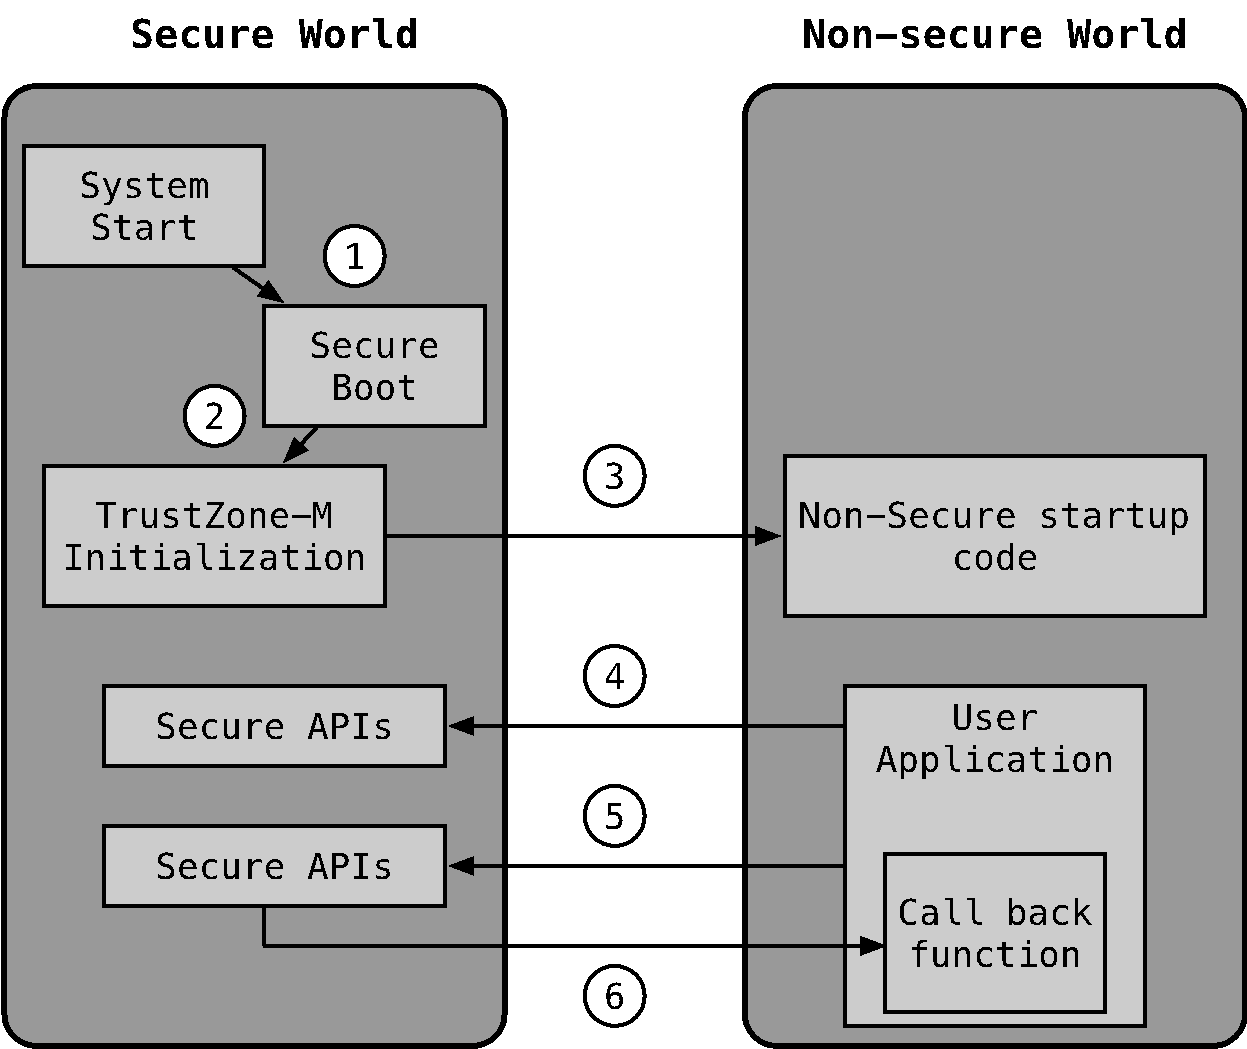
\includegraphics[scale=0.5]{graph/2.png}
    \caption{基于TrustZone-M的系统运行机制}
    \label{fig:TrustZone-M1}
\end{figure}
\par \textbf{资源分配:}TrustZone-M技术为ARMv8-M架构设备提供基于硬件的内存隔离机制,处理器根据内存映射可以对所有资源(包括内存,外设等)进行访问,其内存资源可以设置不同的安全属性以及资源访问控制权限。内存资源可以通过安全属性单元(Security Attribution Unit,SAU)进行安全区域的划分,区域数量由芯片制造商决定,一般为8个区域,SAU只能在处理器处于安全状态下被配置。除SAU之外,安全属性还可以通过实现定义属性单元(Implementation Defined Attribution Unit,IDAU)来进行配置。对某一内存区域来说,其安全属性取决于SAU和IDAU对其配置的共同作用结果,通过对两种配置取逻辑或操作以确定最终的安全属性。此外,内存资源可以通过内存保护单元(Memory Protection Unit,MPU)进行内存访问权限的设置,包括读权限、写权限、可执行权限。任何未遵守该权限要求的访问将会触发HardFault异常处理,安全/非安全世界各有一个MPU。

\par \textbf{异常处理:}在支持TrustZone-M的设备上,通过嵌套向量控制器(Nested Vector Interrupt Control,NVIC)可以设置异常处理为安全或者非安全属性。ARM的M系列处理器在异常处理时支持硬件级的异常上下文保存与恢复。TrustZone-M的异常处理操作模式切换如图\ref{fig: Exception handling operation mode switch}所示,一旦异常被触发,处理器根据向量表(Vector Table)决定异常处理程序并进行控制流跳转,其操作模式自动切换成handler模式并且使用MSP作为异常处理时的栈指针,而异常触发前的上下文信息会自动的压入在先前执行的栈中,称为异常栈帧(Exception Frame)。在ARMv8-M Baseline架构下的异常栈帧的结构如图\ref{fig:Exception frame stack structure}所示\cite{armv8mEaih},包括状态寄存器xPSR、异常返回地址、链接寄存器LR以及通用寄存器R0-R3的值。同时,当前链接寄存器LR将会载入一个称为EXE\_RETURN的特殊值,该特殊值记录着异常返回时处理器的状态信息,如处理器的操作模式、安全状态、使用的栈寄存器等。当异常返回(即跳转至EXE\_RETURN)时,异常栈帧中的内容会自动的载入其对应的寄存器中以恢复异常触发前的上下文,控制流也回到异常触发前的位置继续执行。

\paragraph{基于TrustZone-M的可信执行环境研究应用}
\par 迄今为止,已有相关公司以及研究团队利用TrustZone-M技术提出面向资源受限设备的可信执行环境。Trusted Firmware-M(TF-M)是ARM公司针对ARMv8-M架构(包括Cortex-M23,Cortex-M33,Cortex-M55处理器)或者双核平台提供的一个基于双世界架构(即安全世界和非安全世界)的可信执行环境。它符合ARM公司为物联网嵌入式系统提出的首个行业安全平台架构PSA(Platform Security Architecture)标准,并由ARM公司主导开源。TF-M在ARMv8-M架构上利用TrustZone-M的隔离机制将程序执行环境划分为非安全处理环境(Non-secure Processing Environment,NSPE)以及安全处理环境(Secure Processing Environment,SPE)。在安全处理环境中,TF-M为用户层提供多种安全服务,比如安全启动、安全密钥、安全存储等。其内核层利用SAU以及MPU对安全服务之间进行运行时隔离,并为安全服务之间以及NSPE与安全服务之间提供了安全的通信、安全中断处理等机制,NSPE中的程序可以通过TF-M提供的PSA功能API对安全服务进行调用。然而,用户程序对安全服务进行调用时会进入阻塞直到调用结果返回,这是因为TF-M为满足PSA提出的高等级隔离,TF-M中安全服务的调用模型为信号驱动型且由TF-M内核提供进程间通信(Inter-processing Communication,IPC)机制负责与安全服务进行交互。
\begin{figure}[htbp]
    \centering
    \begin{minipage}[t]{0.45\textwidth} %textwidth值小于0.25,或者linewidth小于0.5,不过这里设置textwidth比设置linewidth效果好一些
        \centering
        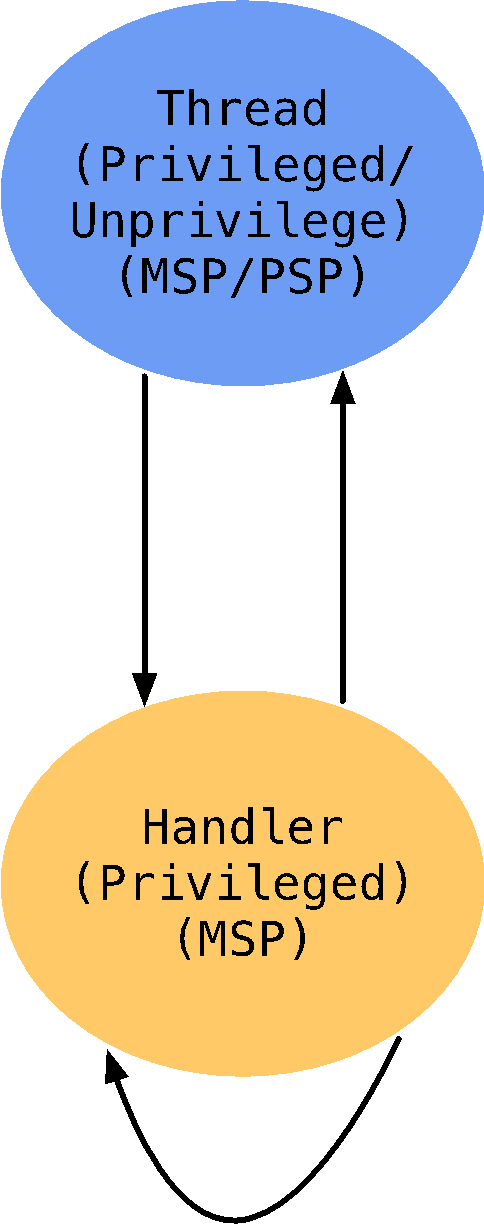
\includegraphics[scale=0.28]{graph/3.png}
        \caption{异常处理操作模式切换}
        \label{fig: Exception handling operation mode switch}
    \end{minipage}
    \hspace{0.50in} % 两图片之间的距离
    \begin{minipage}[t]{0.35\textwidth}%textwidth值小于0.25
        \centering
        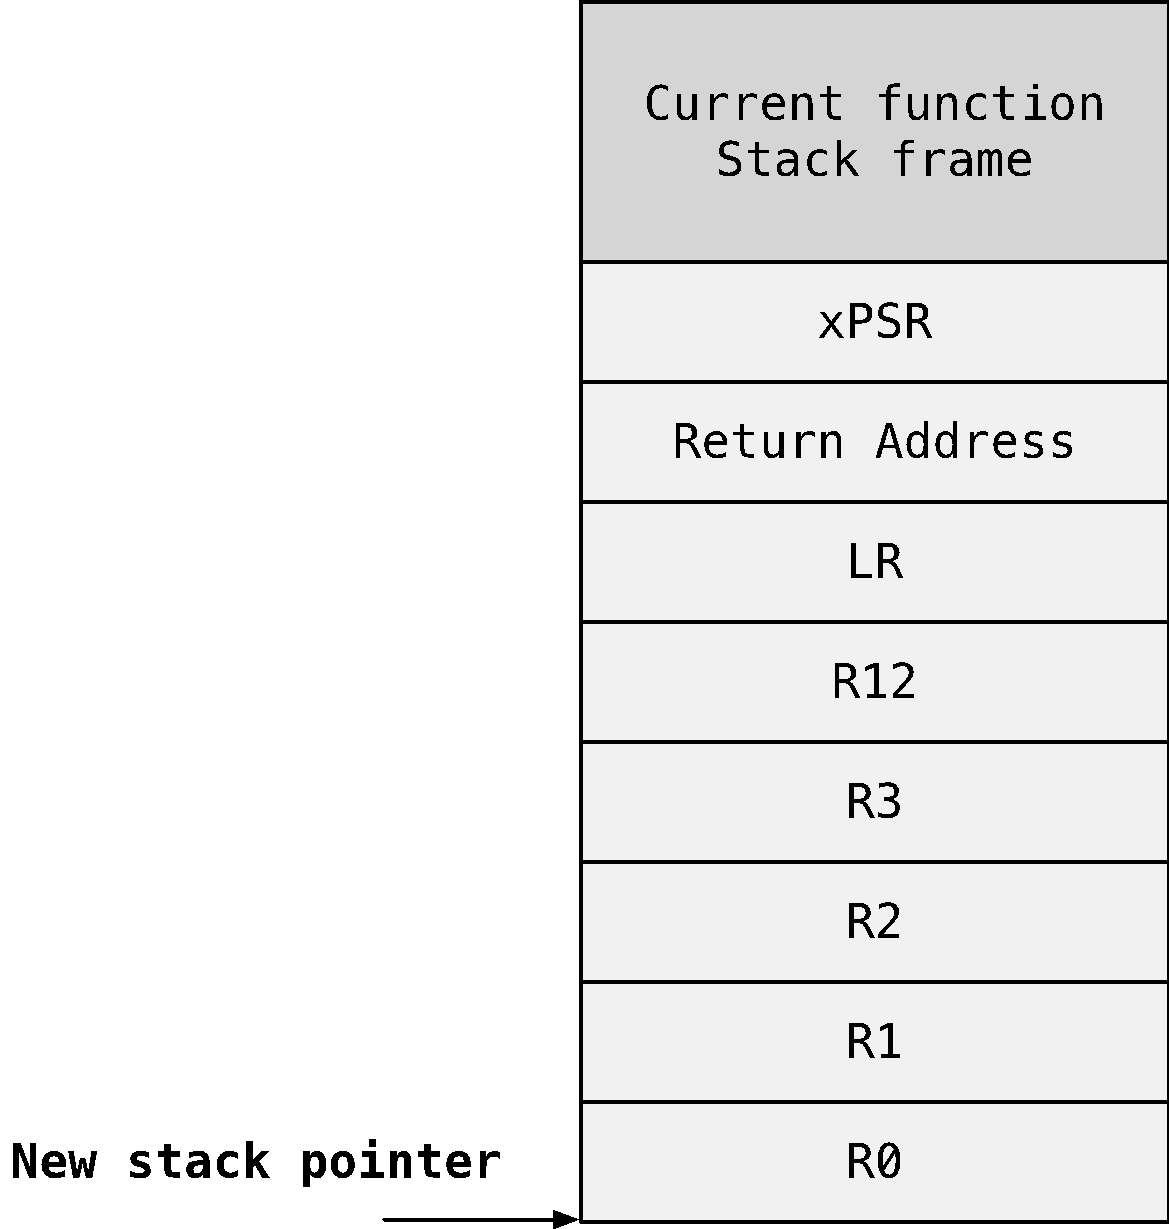
\includegraphics[scale=0.25]{graph/4.png}
        \caption{异常帧栈结构}
        \label{fig:Exception frame stack structure}
    \end{minipage}
\end{figure}
\par Trustonic公司与Microchip公司联手推出了基于TrustZone-M的Knibi-M双世界架构可信执行环境,它针对裸机版本的SAML11\cite{Microchip}设计开发,用于为该设备提供可信的安全服务。它包括内建的密码算法和安全数据存储,可以被集成到支持TrustZone-M的不同微处理器上。Knibi-M利用TrustZone-M以及安全网关(Secure Gateway)\cite{ARMv8-MATO}以与传统的非安全世界应用进行隔离。安全世界包括Knibi-M引导(Bootloader)以及多个安全服务的操作系统,可以为非安全世界中的应用程序提供安全的功能。非安全世界包括主要的应用程序以及调用安全服务的接口。Knibi-M含有一个设备唯一的密钥(目前仅支持SAML11 KPH版本),它是设备出厂时由制造商安装的,它可以为Knibi-M提供消息证明,证明的消息可以被Trustonic的云服务商认证,从而证明该消息来自一个已知的设备。目前,Knibi-M只支持裸机版本SAML11,并不支持其他型号的ARMv8-M设备且未支持实时操作系统。
\par Oliveira\cite{uTango}等人利用TrustZone-M技术,针对ARMv8-M设备提出了基于多世界(Multi-world)架构的可信执行环境操作系统UTANGO。它根据最小权限原则,利用TrustZone-M的安全状态控制器(即SAU或IDAU)降低安全服务的执行权限并使其在非安全世界下执行,并为非安全世界的程序以及各个安全服务提供互相隔离且相同的运行环境,该运行环境称为非安全虚拟世界(Non-secure Virtual World,NSVW)。为了能切换不同的NSVW,每个NSVW都有一个世界控制块(World Control Block,WCB)用于记录其上下文内容,系统运行时UTANGO在安全世界为非安全世界运行的所有NSVW进行调度并为各个NSVW之间提供数据通信接口。然而,由于在世界切换过程中涉及大量的上下文内容保存与恢复,为系统带来较严重的性能开销。另外,目前UTANGO暂不支持抢占式世界切换,非当前NSVW产生的异常难以得到及时的处理,对系统实时性有一定影响。
\par 现有TrustZone-M的可信执行环境的相关工作,其功能主要是为安全服务提供可信的执行环境并为用户提供基于不同安全通信机制的安全服务调用。然而,目前开源可信执行环境中的安全通信机制交互过程复杂,相对于资源和性能受限的低端嵌入式系统来说具有较大代码和性能开销,且可扩展性较差,例如TF-M的信号驱动型安全服务以及IPC的通信机制、UTANGO中NSVW之间繁重的上下文切换等。除此之外,现有基于双世界架构的安全通信机制只允许执行单个安全服务,并未考虑实时操作系统环境下多任务对安全服务进行并发调用需求,导致多任务下对安全服务的调用易受到阻塞,对多任务间的实时协同性产生影响。然而,TF-M以及Knibi-M的安全通信中对安全服务请求过程的参数检查,隔离机制等为本作品设计安全通信机制提供了一种可行思路。另外,本作品针对现有可信操作系统未支持多任务场景下安全服务的并发调用问题,基于现有实时操作系统FreeRTOS,设计多任务场景下对安全服务的并发调用技术。


\subsubsection{Trusted firmware-M可信执行环境}
\paragraph{TF-M简介及设计目的}
\subparagraph{TF-M简介}
\par Trusted Firmware-M(TF-M)是由Arm开发的开源固件作品,旨在为物联网(loT)设备提供安全的运行环境。TF-M旨在提供一个可配置和可裁剪的安全固件平台,以支持从小型嵌入式设备到高端安全系统的多种应用场景。TF-M的架构是模块化的,允许使用者在不影响其他模块的情况下添加或删除安全服务。
\par TF-M 采用了两个核心概念:Secure Processing Environment(SPE)和Non-Secure Processing Environment(NSPE)。SPE 是一个安全执行环境,可以保护关键数据和代码免受未经授权的访问和修改。NSPE 是一个普通的执行环境,可以访问所有的硬件资源。TF-M 提供了一组安全服务,例如安全启动、加密解密、密钥管理、认证和授权等,这些服务可以在SPE中运行,以保证安全性。
\subparagraph{TF-M设计目标}
\par TF-M的设计目标是保护互联网设备上的敏感数据和代码免受攻击,它需要满足以下需求:
\begin{itemize}
    \item 安全性:TF-M 旨在为 IoT 设备提供安全的运行环境,以保护设备和用户数据免受攻击。
    \item 可配置性:TF-M 的架构是模块化的,允许用户根据自己的需求配置和定制安全服务。
    \item 易于集成:TF-M 提供了一个标准接口,使得其他软件可以轻松地与TF-M 集成。
    \item 可移植性:TF-M 可以在不同的硬件平台上运行,并且支持多种处理器体系结构。
    \item 易于维护:TF-M 的代码是模块化的,易于理解和维护。
\end{itemize}

\paragraph{TF-M系统设计}
\subparagraph{TF-M架构设计}
\par TF-M的系统整体架构设计如下图\ref{readme_tfm_v8.png}所示。整个TF-M部署在安全世界(SPE)中,为安全/非安全世界提供安全服务,主要由安全启动(Secure Boot)、TF-M内核(TF-M Core)以及安全服务(Secure Service)组成。
\begin{figure}
    \centering
    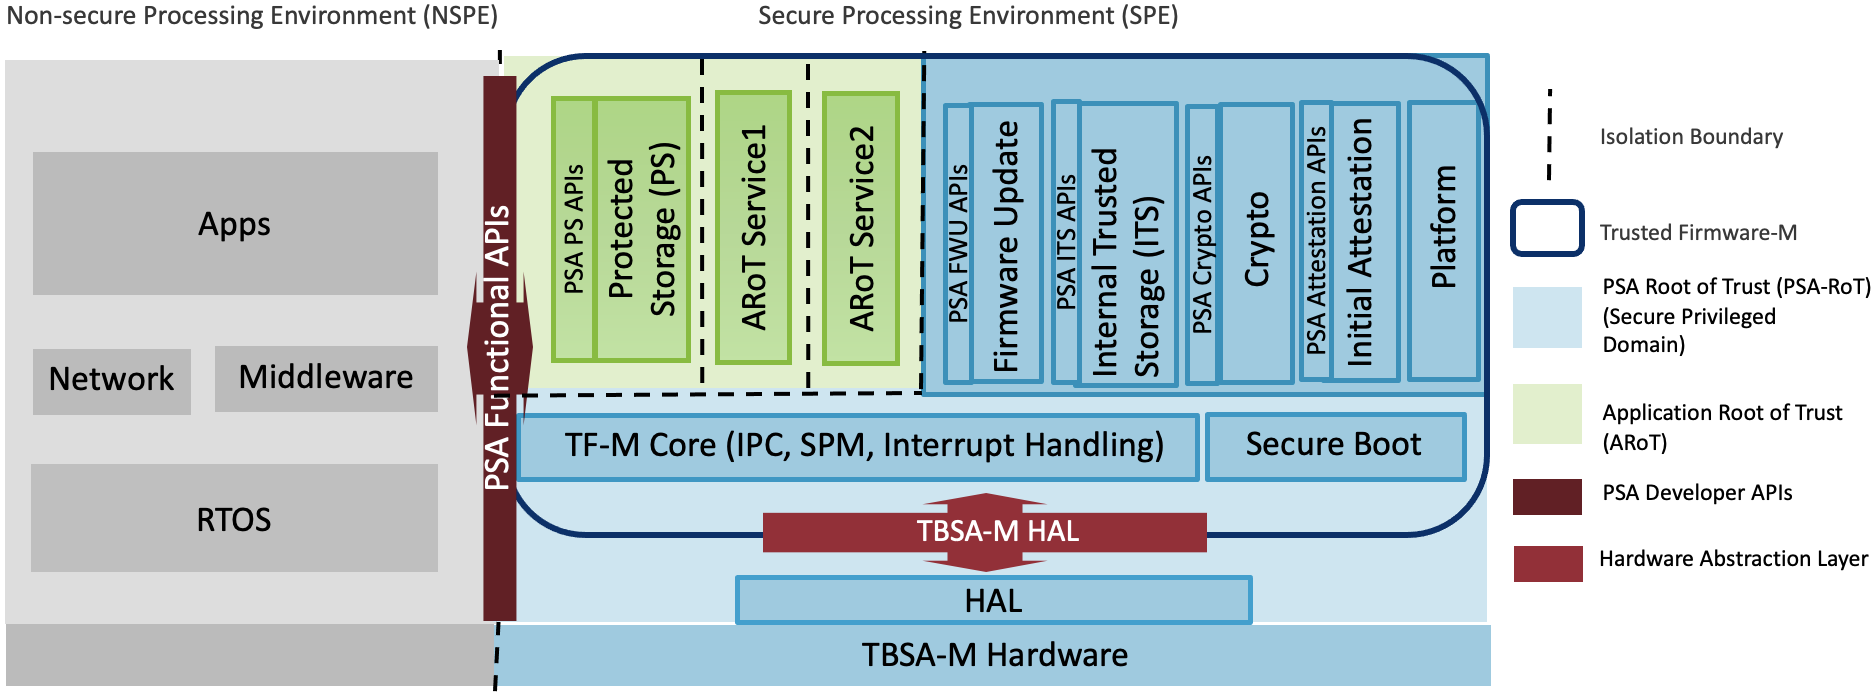
\includegraphics[scale=0.2]{graph/readme_tfm_v8.png}
    \caption{Trusted Firmware-M架构图}
    \label{readme_tfm_v8.png}
\end{figure}
\par 在Trusted Firmware-M的背景下,安全启动负责在固件映像被加载和执行之前验证其真实性和完整性。它通过根据设备安全引导固件中存储的一组受信任的密钥检查固件映像的数字签名来执行此验证。安全启动可以对SPE (Secure Processing Environment)和 NSPE (Non-Secure Processing Environment)固件映像进行身份验证。NSPE映像在设备的非安全世界中执行,而SPE映像在安全世界中执行。如果固件映像未通过Secure Boot验证,则会被拒绝,设备将无法执行它。这可以防止攻击者在设备上执行未经授权的代码,从而保护设备及其数据免受恶意活动的侵害。
\par TF-M内核是TF-M的主要组成部分之一,它是一个基于微内核的安全操作系统内核。TF-M core的主要功能是提供安全隔离、通信控制和安全执行,主要模块包括IPC、SPM、Interrupt Handling。其中,IPC 用于在SPE和 NSPE之间进行通信。它提供了一种安全的方式,以便在受保护的环境内传递数据和控制信息。SPM用于管理和控制在SPE中运行的各个安全分区。SPM使得多个安全分区可以在同一硬件平台上运行,并且可以互相隔离。Interrupt Handling用于管理和处理来自设备的中断请求。TF-M内核通过在SPE和NSPE之间传递中断请求,确保了所有中断的安全处理。TF-M内核还包括一些其他的辅助模块,比如Secure Entry/Exit和Secure Attribution等,用于在SPE和NSPE之间进行安全的上下文切换和资源分配。
\par 安全服务负责向安全/非安全世界提供具有较高安全需求的功能实现并由安全内核负责对其进行调用,如安全储存、安全启动、加密等。每一个安全服务具有唯一标识符SID(Service ID)且有统一的函数调用入口。为统一调用接口,每个安全服务都可以通过SID和version两个参数被非安全世界用户进行调用,其中,SID参数是要调用的安全服务的唯一标识符,version是请求的信任根服务版本。NSPE的用户通过PSA API发送请求后,由SPM将请求打包成消息并转发到相应服务处理程序的函数。
\par TF-M拥有特定的隔离机制,以保护一个保护域的信息免受从其他域访问,故TF-M中不同区域间的访问需要特定的PSA API来实现,后续将详细解释TF-M的通信机制。

\subparagraph{TF-M隔离机制}
\par PSA针对不同设备的安全性、性能、成本提出了三个级别的隔离,如下图\ref{TFM isolation}所示。第一级隔离将SPE与NSPE隔离开,NSPE不能访问SPE的资源,需要由PSA client API访问特定的服务。第二级隔离在第一级隔离的基础上,引入了PSA RoT和Application RoT隔离边界。这两类服务不能访问各自的资源,需要由PSA API访问对方的服务。第三级隔离在前两级的基础上引入了对每个安全分区之间的隔离边界,实现对所有安全分区的隔离,其是最高级别的隔离。
\begin{figure}
    \centering
    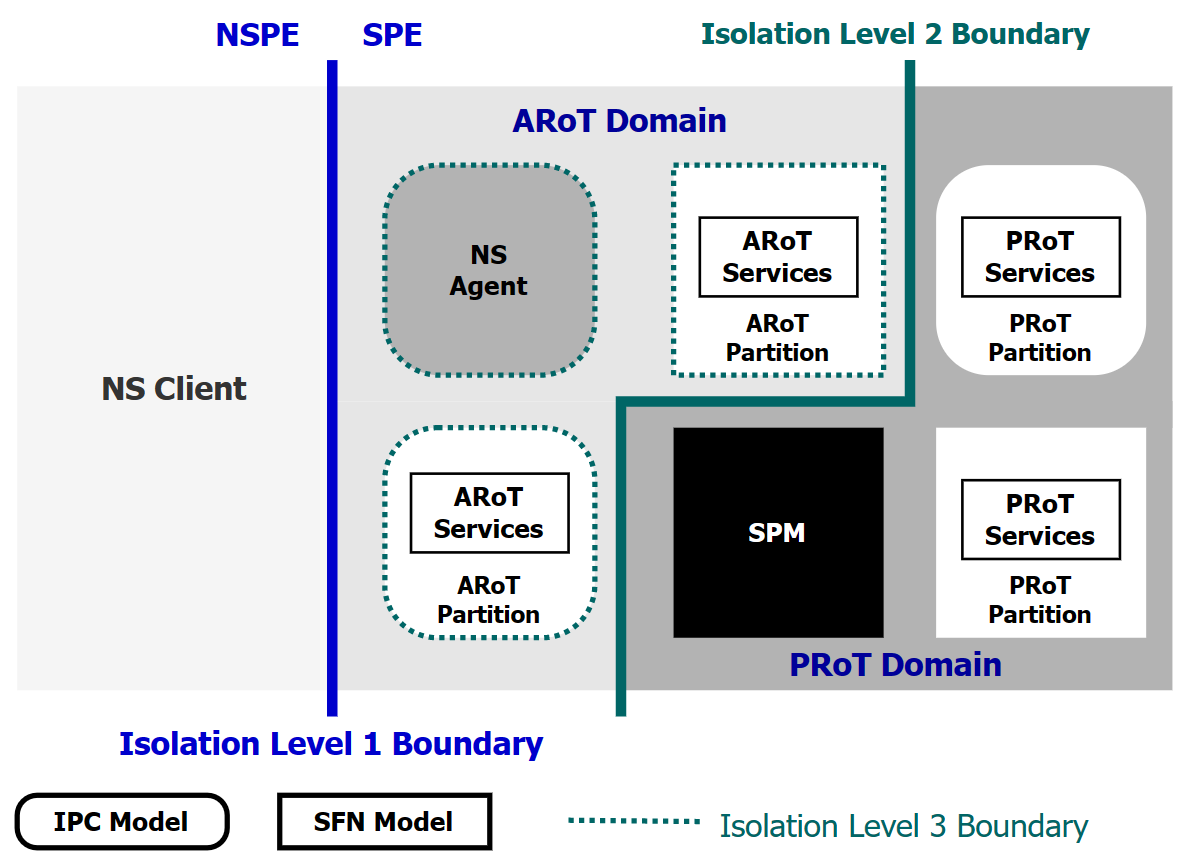
\includegraphics[scale=0.27]{graph/isolation.png}
    \caption{TF-M隔离机制}
    \label{TFM isolation}
\end{figure}
\subparagraph{TF-M提供的安全服务}
\par Trusted firmware-m提供了一系列安全服务来保护设备和应用程序的安全,以下简要介绍一些TF-M提供的安全服务:
\begin{itemize}
    \item 安全更新(Secure Firmware Update):提供了对设备固件的安全更新和回滚功能,以确保固件的完整性和真实性。
    \item 安全存储(Secure Storage):提供了一个安全的存储区域,用于保存设备的机密信息,例如密钥和证书。
    \item 安全连接(Secure Connection):提供了一些加密和认证技术,用于建立安全的设备到设备(Device-to-Device)或设备到云(Device-to-Cloud)连接。
    \item 安全运行时环境(Secure Runtime Environment):提供了一个隔离的安全环境,在这个环境中执行的代码和数据与其他非安全代码和数据隔离开来。
    \item 安全调试(Secure Debug):提供了一些安全的调试技术,以便开发人员在不破坏设备安全性的情况下对设备进行调试和测试。
    \item 安全网络协议(Secure Network Protocols):提供了一些安全的网络协议,例如TLS和DTLS,用于保护设备与其他设备或云服务之间的通信安全。
    \item 安全固件(Secure Firmware):提供了一些安全的固件实现,例如安全的虚拟化技术,以确保设备的安全性。
    \item 安全证书管理(Secure Certificate Management):提供了一些安全的证书管理技术,以确保设备的证书的安全性和完整性。
    \item  安全启动(Secure Boot):用于验证启动代码的完整性和真实性,确保只有受信任的代码被执行。
\end{itemize}
这些安全服务可以根据设备的需求进行配置和组合,以实现设备的安全性和可信度。

\subparagraph{安全分区运行机制——SFN模式与IPC模式}\par TF-M 实现了 PSA-FF-M 定义的IPC和SFN机制,以允许隔离固件分区之间的通信。IPC model和SFN model的主要区别如下:
\begin{itemize}
    \item IPC(Inter-Process Communication)模型是一种进程间通信模型,它允许不同的进程之间相互通信和协作,从而共同完成任务。TF-M中的IPC Model使用的是基于消息队列(Message Queue)的方式进行通信。每个安全服务都有一个消息队列,其他安全服务可以向该队列发送消息,通过消息队列,安全服务可以实现相互通信和协作。TF-M提供的安全启动、安全调试、安全存储等安全服务均采用IPC模式。
    \item SFN(Secure Function Call)模型是一种基于函数调用的安全模型,它允许不同的安全服务之间进行直接的函数调用。在TF-M中,安全服务被封装为一系列的安全函数,这些函数可以被其他安全服务直接调用,从而完成相应的安全操作。为了确保安全性,每个安全函数都被封装在一个受保护的安全域中,只有在该安全域中的安全服务才能调用该函数。TF-M提供的初始证明服务、加密、固件更新等安全服务均采用SFN模式。
\end{itemize}
IPC模式和SFN模式都是用于不同安全服务之间的通信和协作模式,IPC模式使用消息队列进行通信,更加灵活和可扩展,但安全性较差。SFN模式使用函数调用进行通信,安全性较好,但不太灵活。用户在自行编写添加安全服务时,具体选择哪种模型取决于应用场景的需求和安全性要求。

\subparagraph{TF-M架构中的各类API}
\par Trusted Firmware-M(TF-M)架构中包含了一系列的API,用于实现安全功能和提供安全服务。以下是TF-M架构中一些重要的API及其功能的详细介绍:
\begin{itemize}
    \item SST(Secure Storage Service)API:提供了对安全存储的访问和管理。SST API允许应用程序安全地读取、写入和删除存储在安全存储区域中的数据。
    \item ITS(Initial Trusted Service)API:用于设备的安全启动过程。ITS API提供了验证引导程序完整性、加载和执行可信固件的功能。它确保只有经过验证的固件能够在安全环境中启动。
    \item PSA(Platform Security Architecture)API:提供了一组通用的安全服务接口,用于实现设备的安全功能。PSA API包括加密、身份验证、安全认证、随机数生成等功能,可供应用程序使用。
    \item RoT(Root of Trust)API:用于建立设备的根信任,提供安全隔离和保护关键功能和数据的能力。RoT API用于创建和管理安全分区,确保关键代码和数据只能在受信任的环境中执行和访问。
    \item IPC(Inter-Processor Communication)API:用于在安全世界和非安全世界之间进行受控的通信。IPC API定义了安全接口,允许安全世界与非安全世界之间进行安全的数据传输和交互。
    \item Secure Partition Manager(SPM)API:用于管理和控制安全分区的运行。SPM API允许安全分区之间的隔离,并管理它们之间的资源分配和通信。
    \item Secure Gateway API:提供了对安全网关功能的访问,用于安全地与外部环境进行通信。Secure Gateway API允许安全世界与外部设备或网络进行加密通信和安全数据交换。
    \item Secure Debug API:用于在安全模式下进行调试和故障排除。Secure Debug API提供了安全的调试接口,允许对安全世界进行调试操作,同时保护关键数据的机密性和完整性。
\end{itemize}
\par 以上是TF-M架构中的一些重要API,它们提供了安全功能和服务的接口,用于实现物联网设备的安全性和可信度。通过使用这些API,开发者可以构建安全的应用程序和服务,保护设备免受各种安全威胁。

\subparagraph{TF-M源码文件夹结构分析}
\par 在TF-M的源码库中,有许多子文件夹,包括:
\begin{itemize}
    \item bl1:包含用于生成TF-M的第一级引导程序(BL1)的代码。此文件夹中的代码用于初始化系统环境并引导BL2。
    \item bl2:用于生成TF-M的第二级引导程序(BL2)的代码。此文件夹中的代码用于生成TF-M的第二级引导程序(BL2),该程序用于引导TF-M并配置系统环境。
    \item secure\_fw:包含实现安全功能的代码,如安全监控器和安全服务。此文件夹中的代码是实现TF-M核心安全功能的代码,包括安全状态机、安全中断处理、安全事件处理等。
          \begin{itemize}
              \item include:包含了一些必要的头文件,这些头文件定义了在    TF-M中需要使用的函数和变量等。
              \item partitions:用于将TF-M固件划分为不同的分区,每个分区都拥有自己的内存和安全级别。在这个文件夹中,开发者可以定义各个分区的大小和访问权限等。
              \item shared:包含了一些可供不同分区共享的资源,比如共享内存区域,共享的全局变量等。这些共享的资源在不同分区之间进行数据传输时需要进行安全性的保护。
              \item spm:安全分区管理器(Security Partition Manager)的缩写,是TF-M中一个重要的组件。spm文件夹中包含了spm的代码和配置文件,spm负责在不同的分区之间进行数据传输和安全性控制,以确保系统的安全性和可靠性。
          \end{itemize}
    \item interface:该文件夹包含与TF-M外部接口相关的代码,如TF-M API和外部接口函数。此文件夹中的代码是与外部系统的接口代码,包括TF-M提供的API函数、设备驱动程序接口、系统调用接口等。
          \begin{itemize}
              \item include:包含了一系列的头文件,这些头文件是开发者在使用TF-M时需要包含的文件,其中定义了TF-M的API接口、数据类型、错误码等信息,开发者可以使用这些头文件来编写TF-M的客户端代码,调用TF-M的API接口实现安全功能。
              \item src:开发者在使用TF-M时需要引用的文件,其中实现了TF-M的API接口,开发者可以使用这些源文件来实现TF-M的服务端代码,提供安全功能服务。
          \end{itemize}
    \item lib:用于实现基本安全功能的库代码,如加密算法和哈希函数。此文件夹中的代码是用于支持安全服务的基本库函数,如随机数生成、哈希计算、加密解密算法等。
    \item tools:包含用于开发和调试TF-M的实用工具和函数信息自动提取工具。例如,此文件夹中包含了与TF-M相关的调试工具、测试脚本以及用于生成密钥和证书的工具等。
    \item platform:包含与平台相关的代码,如设备启动代码和外设驱动程序。此文件夹中的代码是为了支持不同的硬件平台,使TF-M能够运行在不同的处理器架构和芯片上。
    \item docs:TF-M的文档,如用户手册和开发人员指南。此文件夹中的文件包括各种文档、说明、手册等,用于指导开发人员使用TF-M进行开发。
    \item cmake:用于生成TF-M构建系统的CMake文件。此文件夹中的文件用于支持TF-M的自动化构建,包括CMake脚本和Makefile文件。
    \item config:用于配置TF-M的各种选项的配置文件。此文件夹中的文件用于配置TF-M的相同选项,如安全级别、存储器布局、加密算法、硬件平台等。
\end{itemize}

\paragraph{安全/非安全世界安全通信机制}
非安全世界在调用安全世界的安全服务时,其整个通信过程如下图\ref{TF-M Secure communication processes}所示,可以分为三个阶段:(1)请求阶段:非安全世界任务发起安全服务的请求至特定的API并最终交给TF-M内核;(2)执行阶段:TF-M内核验证客户端的身份和权限,然后根据请求中指定的安全服务标识符,将请求转发给对应的安全服务并等待其响应结果;(3)响应阶段:安全服务执行结束并返回执行结果给 TF-M内核,TF-M内核收到安全服务的执行结果后,会根据请求的类型和参数,将结果通过特定API返回给客户端。
\begin{figure}
    \centering
    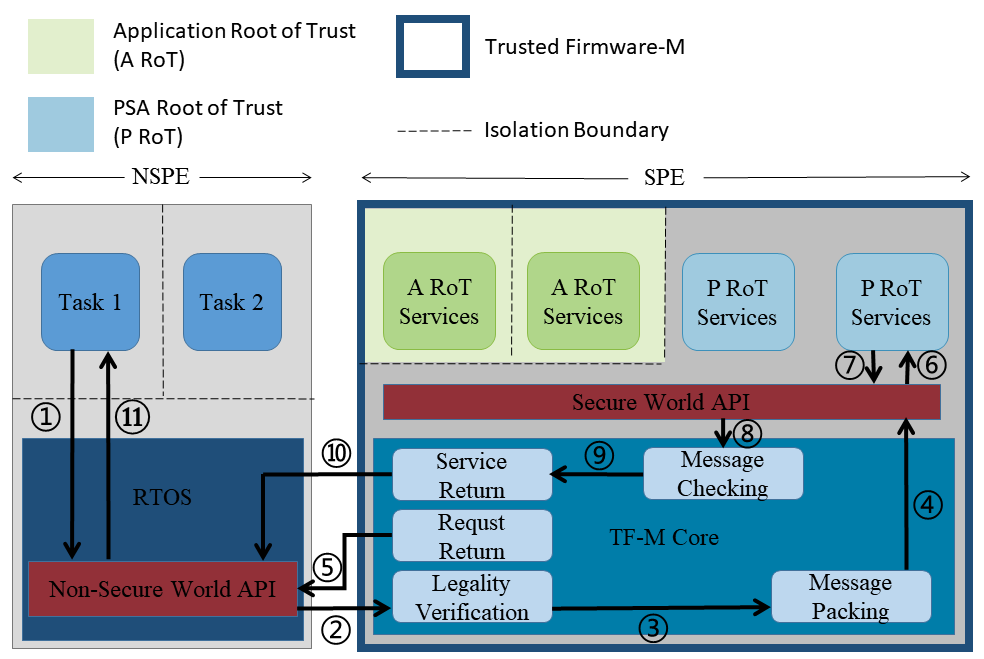
\includegraphics[scale=0.38]{graph/TF-M Secure communication process.png}
    \caption{TF-M调用机制}
    \label{TF-M Secure communication processes}
\end{figure}

\subparagraph{请求阶段}
\par 客户端首先向 TF-M 提供的API接口发送请求。这些API接口包括tfm\_spm\_request(), tfm\_ns\_interface\_dispatch(), tfm\_secure\_api\_call()等。客户端发送的请求中包含要调用的安全服务的标识符,以及传递给安全服务的参数等信息,这些参数信息可以包括数据结构、指针等。之后,TF-M内核会接收客户端发送的请求,并在请求合法性验证通过后,根据请求中指定的服务标识符,选择相应的安全服务进行调用。在完成安全服务调用后,TF-M 内核会向客户端返回相应的结果,其中可能包括表示安全服务调用状态的状态码、加解密的数据、安全服务抛出的异常或中断等。客户端可以通过 API 接口获取 TF-M内核返回的结果信息。
\par 上述过程中,TF-M内核在接收到API调用请求后,为防止有攻击者通过构造参数等方式对安全服务进行恶意调用,利用安全服务以访问安全世界的重要数据,会首先检查客户端的请求是否合法,检查包括以下内容:
\begin{itemize}
    \item 验证请求的来源:TF-M core会验证请求的来源,确保请求来自于受信任的客户端。这个过程可以通过验证请求中包含的认证信息,例如数字签名、证书等方式来完成。
    \item 验证请求的完整性:TF-M内核会验证请求的完整性,以确保请求的内容没有被篡改或者修改。这个过程可以通过使用消息认证码(MAC)等机制来完成。
    \item  验证请求的合法性:TF-M内核会验证请求是否合法,即请求中包含的安全服务标识符和参数是否合法。这个过程可以通过检查请求中包含的参数和标识符是否符合安全策略和规则来完成。
    \item  验证请求的访问权限:TF-M内核会验证请求的访问权限,即请求的客户端是否具有调用该安全服务的权限。这个过程可以通过检查请求的客户端身份和权限等信息来完成。
    \item  验证请求的时序性:TF-M内核会验证请求的时序性,即请求是否按照正确的顺序到达。这个过程可以通过使用时间戳等机制来完成。
\end{itemize}
\par 通过对请求进行上述合法性验证,TF-M内核可以确保安全服务的调用是合法、可信和安全的,同时避免了可能导致安全漏洞和风险的请求。

\subparagraph{执行阶段}
\par 合法性验证之后,TF-M内核将请求的参数和其他相关数据打包成一个消息。消息包括要调用的安全服务的标识符,以及传递给安全服务的参数等信息。在打包过程中,TF-M内核会将消息进行加密和签名,以确保消息的机密性和完整性。之后,TF-M内核使用安全的通信机制将消息发送到安全分区。这个机制会在TF-M内核和安全分区之间建立的安全通信通道,它可以使用一些安全协议,例如TLS、IPsec等来保护通信的机密性和完整性,同时确保通信的可靠性。这个过程可以使用一些底层硬件设施来实现,例如硬件加速模块、安全内核等。安全分区接收到请求消息后,会对其进行解包。解包过程中,安全分区会验证消息的完整性和机密性,并使用相应的密钥解密消息内容。如果消息的完整性和机密性验证失败,安全分区会拒绝执行请求,否则,安全分区会继续执行请求。
\par 之后,安全分区根据请求中包含的标识符调用相应的安全服务,并传递相应的参数。在执行安全服务期间,安全分区可能会访问安全世界内的受保护资源,例如受保护的存储器、设备等。安全分区会使用安全策略和机制来确保这些资源不会被非安全世界访问或破坏。
\subparagraph{响应阶段}
\par 在安全服务执行完成后,安全分区将执行结果打包成一个响应消息。响应消息包括响应码、执行结果以及其他必要的信息。之后,安全分区使用安全通信机制将响应消息发送回TF-M内核。TF-M内核接收到安全的响应消息后,首先对其进行验证。验证包括检查消息的签名和校验和,以确保消息的完整性和真实性。如果消息验证失败,则TF-M内核会丢弃消息并返回错误码。
\par 如果消息验证成功,则TF-M内核将解包响应消息,获取其中的执行结果和其他相关信息。最后,TF-M内核将响应结果返回给客户端。客户端收到响应结果后,可以进行下一步操作。
\par 需要注意的是,TF-M内核在处理响应消息时,需要使用与请求消息相同的安全通信机制。这是因为安全通信机制是建立在会话级别的,如果使用不同的通信机制,可能导致安全通信中断,从而使得通信变得不可靠。

\paragraph{TF-M应用研究}
\par 2016年,P. Wägemann等人\cite{trustzone-firmware}设计和实现一种基于TrustZone的安全固件架构,利用TF-M作为基础来保护物联网设备免受各种攻击。该安全固件架构基于TrustZone技术,该技术提供了硬件级别的安全隔离。研究者利用TrustZone的两个不同的执行环境,即"安全世界"和"非安全世界",来实现安全隔离。安全世界运行在受保护的安全模式下,而非安全世界则运行在常规的非安全模式下。通过使用TrustZone和TF-M,研究者实现了更强大的安全隔离。安全世界被限制为只能通过安全接口与非安全世界进行通信,这确保了安全世界的代码和数据无法被非安全世界访问或篡改。安全世界中的关键功能和数据被保护在一个安全的容器中,只有经过授权的访问才能获取。为了保护设备中的关键数据和执行,研究者采取了多种安全措施。首先,通过在安全世界中运行关键功能,确保只有经过授权的代码可以访问和执行这些功能。其次,使用加密算法对关键数据进行加密,以防止未经授权的访问。此外,安全世界中的代码和数据也可以受到完整性检查的保护,以确保其未被篡改。但这项研究可能存在一些实施上的挑战。例如,由于物联网设备的资源限制,安全固件的实现可能会受到性能和存储限制的影响。此外,研究中可能没有对所有可能的攻击进行全面考虑,导致可能存在其他安全漏洞。
\par S.Kumar等人进行的研究\cite{secure-firmware-updates}旨在解决物联网设备固件更新过程中的安全性问题。研究者提出了一种安全的固件更新机制,利用ARM TrustZone和TF-M来确保固件的完整性和机密性。他们采用了多种机制来防止恶意固件的注入。首先,实现了固件验证机制,通过数字签名或哈希算法对固件进行验证,确保固件的完整性。只有通过验证的固件才能被接受和安全地更新。其次,实现身份认证机制用于验证固件的来源和合法性,以防止非法固件的注入。这可以通过使用公钥基础设施(Public Key Infrastructure)或其他身份验证机制来实现,确保请求只有来自信任的源头才能被接受。通过使用ARM TrustZone和TF-M,研究者确保了固件更新过程的安全性。安全世界中的代码负责处理固件更新的操作,并通过安全接口与非安全世界进行通信。固件在安全世界进行验证和认证后,才能被接受并安全地更新到设备中。这样可以防止未经授权的固件更新,同时确保更新的固件是合法和可信的。但本研究实现的安全固件更新机制在实现过程中无法确保在固件更新过程中,包括固件的验证、加载和替换过程的所有环节都是安全的。
\par  Arm Limited 公司\cite{trusted-firmware}基于前人的研究,为物联网设备提供一个全面的安全框架,提供了全面的安全功能应用,以应对不断增长的安全威胁。Arm Limited 的研究方案主要集中在设计和实现 TF-M 的安全特性和功能。这些功能包括安全引导(Secure Boot)、安全分区(Secure Partitioning)和安全通信(Secure Communication)等。相较于以往的研究,Arm Limited 在 TF-M 的研究中取得了一些突破。他们提供的全面安全框架集成了安全引导、安全分区和安全通信等关键功能,使得物联网设备能够综合地应对安全挑战。其次,他们基于 Arm Cortex-M 架构,充分利用硬件安全特性和 TrustZone 技术,提供了更强大的安全隔离和保护机制。但是,尽管 Arm Limited 的研究提供了一个全面的安全框架,但也存在一些限制和挑战。例如,由于物联网设备的多样性和复杂性,将该安全框架应用于不同设备可能需要定制化的适配和配置,这将增加了开发和部署的复杂性。此外,该研究可能没有充分考虑到未来可能出现的新型安��威胁和攻击方式。
\par J. Kim等人的研究\cite{secure-bootloader}旨在设计一种基于 TF-M 的安全引导程序,以提供物联网设备的安全引导功能。研究者设计了一个基于 TF-M 的引导程序,该程序能够确保设备在启动过程中的安全性,并保护设备免受恶意固件的加载和执行。研究者利用 TF-M 提供的安全特性,如安全分区和安全存储,来实现安全引导过程。安全隔离使引导程序运行在安全分区中,与非安全分区进行隔离。这样可以防止恶意固件或非授权代码对系统的攻击和篡改。只有通过授权的引导程序可以加载和执行,确保引导过程的完整性和可信性。安全验证使引导程序和关键数据存储在安全存储中,并通过安全存储的保护机制进行访问控制。在引导过程中,TF-M可以验证引导程序的完整性和真实性,确保只有经过验证的固件被加载和执行。然而,这项研究还存在一些潜在的缺陷和不足,比如如何确保引导程序的完整性和可信性,以及应对物理攻击和侧信道攻击的挑战。此外,实施安全引导可能需要额外的硬件支持或安全认证机制,将增加设备的成本和复杂性。

\subsubsection{研究现状总结}
\par 现有研究工作在面向内存破坏攻击的通用系统防御技术,基于TrustZone-M技术的可信执行环境构建技术以及面向低端嵌嵌入式系统的内存破坏防御技术方面都已取得一定的进展和成果,发现不同的技术均有其优缺点,对本作品研究工作的开展有很大的借鉴价值,现状总结如下:
\begin{itemize}
    \item[(1)]常见的面向低端嵌入式系统的攻击有ROP攻击、缓冲区溢出、格式化字符串等。ROP攻击是一种利用程序中已存在的代码片段(称为gadget)构建恶意代码的技术。缓冲区溢出则是指当向有限大小的缓冲区写入超过其容量的数据时,数据会溢出到相邻内存区域,导致数据覆盖和执行流程异常。格式化字符串漏洞是指当程序中的格式化字符串函数(如printf)使用不当时,攻击者可以利用格式化字符串参数来读取或写入内存的任意位置。
    \item[(2)] 现有地址空间隐藏技术均存在安全隐患。由于基于启动阶段的软件多样化技术并未对多样化部署代码进行多样化且缺乏可信根(Root of Trust) ,因此无法保证其自身的可信,攻击者可能利用该代码执行代码复用攻击以破坏系统安全性;基于编译阶段的多样化技术由于资源限制具有较小随机嫡,且其易受到暴力破解攻击。XOM技术通过运行时无法对固件进行读取从而防御地址空间信息泄漏,然而其与编译阶段的多样化技术一样,无法防御离线固件读取攻击,比如OTA更新时的固件泄漏攻击。
    \item[(3)] 地址空间布局随机化(ASLR)是一种从另一个角度保护系统的安全技术,通过随机化内存布局增加攻击者的难度。ASLR依赖操作系统支持,在系统启动时对内存区域的基址进行随机化,破坏攻击者对特定地址的依赖。然而,在嵌入式系统中,由于地址空间小,没有加载器等硬件条件限制,ASLR 技术难以实施。
    \item[(4)] 当前针对TrustZone-M技术的TEE OS研究尚处于起步阶段,其安全通信机制在设计上存在安全冗余,对低端嵌入式系统具有较大性能开销。此外,现有技术针对安全服务调用暂不支持多任务并发,影响系统多任务实时协同。
    \item[(5)] 基于TrustZone和TF-M的研究为物联网设备提供了安全保护。通过安全世界和非安全世界的隔离,安全功能和数据得到保护。在固件更新方面,采用数字签名和身份认证机制确保固件的完整性和合法性。Arm Limited的研究提供了全面的安全框架,集成了安全引导、分区和通信等功能。安全引导程序利用TF-M的特性实现了安全启动,保护设备免受恶意固件的加载。然而,该研究在实施上仍面临资源限制、新型攻击和复杂性等挑战。
\end{itemize}
\subsection{作品意义与目标}
\par 近年来,随着智能家居的广泛普及、智慧城市的深入部署,数以百万计的物 联网设备正加速万物互联时代的到来。然而,其中很大一部分物联网设备是基于微控制器实现的低端嵌入式系统,由于其硬件资源不足、计算能力受限等特点,使其极易受到来自内存破坏引起的安全威胁,尤其是控制流劫持攻击,因此维护其安全性近年来受到广泛关注。
\par 目前抵御内存破坏对低端嵌入式系统的安全威胁主要有以下几个挑战:
\begin{itemize}
    \item 有限的内存资源:低端嵌入式系统通常内存资源非常有限,因此内存保护机制需要在尽可能小的内存开销下提供有效的安全保护。
    \item 嵌入式程序多样性:嵌入式程序多由独立平台设计,代码结构复杂多样,内存保护机制可扩展性较差。
    \item 处理器性能限制:低端嵌入式系统通常采用的是低功耗处理器,其处理能力有限,因此内存保护机制需要在不影响系统性能的前提下实现。
    \item 实时性保证:低端嵌入式系统通常需要实时响应各种事件,因此内存保护机制需要在不影响系统实时性能的前提下实现。
\end{itemize}
\par 鉴于低端嵌入式系统所面临的安全挑战,近年来如何提高其安全性已经引起广泛关注。目前,有三个主要方向用于提高低端嵌入式系统的安全性:首先是利用低端嵌入式系统的硬件设施,实现内存隔离、内存检测和访问控制等安全防护措施。然而,由于嵌入式系统硬件的多样性,这要求系统开发者针对不同硬件环境实现相应的安全机制,导致可扩展性较差。此外,还需额外的硬件支持,从而增加成本和工程开销。第二个方向是利用编译器技术,在对代码进行词法和语法分析后,在重新编译现有嵌入式系统源码的过程中加入额外代码以实现特定的防御机制,从而提高系统安全性。这种方法的优点是无需更改原有系统的软硬件,避免了成本和工程开发上的额外开销。但是,由于编译器在软件层面提高系统安全性,因此可能会给代码的执行效率和性能带来额外负担。
\par 最后一个方向是综合前两者,通常针对已有可信硬件的低端嵌入式系统在编译过程中加强代码安全性,可将支持可信硬件的防御机制代码直接编译至目标代码,具有较好的可扩展性。由于此类方法本质上仍然基于编译器对代码进行重新编译,因此对系统开发具有较好的透明性。同时,得益于可信硬件的支持,对嵌入式系统的安全性以及性能也有较好的兼顾。 
\par 本作品借鉴第三个方向的思路,针对低端嵌入式系统的控制流劫持攻击设计实现了基于ARM TrustZone-M 的函数级动态随机加载技术。我们对现有实时操作系统FreeRTOS以及可信执行环境操作系统Trusted Firmware-M进行了针对性的设计。利用自动化工具实现对系统以及函数信息的高效收集与灵活管理,实现函数运行时的实时状态感知。同时在FreeRTOS和Trusted Firmware-M源代码的基础上进行修改,在安全世界中引入地址空间布局随机化机制,使每个函数能够被加载至随机化区域并恢复运行。之后,移植Trusted Firmware-M使其能够在STM32L562开发板上与FreeRTOS协作运行,并从非安全世界实现对安全世界中地址空间布局随机化服务的调用,对整个代码空间(包括用户程序以及实时操作系统内核)实现了函数级随机化,从而实现对低端嵌入式系统的全面保护。
\par 此外,本作品针对性能和内存设计了相应的优化机制。在性能方面,针对函数加载引起的性能开销问题,设计针对函数加载的缓存技术,将随机化操作较多的函数放入缓存块中,并利用缓存预取和缓存命中率提高等技术手段,以提高系统的运行效率。
\par 在内存方面,为了解决低端嵌入式系统中内存资源受限问题,本作品还提出了一个函数级随机化内存管理机制,用来实现高效的内存管理并防御内存破坏的攻击。具体来说,这个机制通过收集函数信息并进行动态随机化加载,确保每次函数运行时的内存地址都不同,从而有效地防御了ROP攻击。此外,该作品设计内存回收机制实现了对内存资源的高效利用,减少了内存碎片的产生,提高了内存使用效率。通过这些手段,函数级随机化内存管理机制能够在保证系统安全性的同时,尽可能地减小内存开销,提高系统性能。
\par 我们的作品针对低端嵌入式系统的控制流劫持攻击设计实现了基于 ARM TrustZone-M 的函数级动态随机加载技术。我们对现有实时操作系统 FreeRTOS 以及可信执行环境操作系统 Trusted Firmware-M 进行了针对性的设计。利用自动化工具实现对系统以及函数信息的高效收集与灵活管理,实现函数运行时的实时状态感知。同时在 Free RTOS 和 Trusted Firmware-M 源代码的基础上进行修改,在安全世界中引入地址空间布局随机化机制,使每个函数能够被加载至随机化区域并恢复运行。之后,移植 Trusted Firmware-M 使其能够在 STM32L562开发板上与 FreeRTOS 协作运行,并从非安全世界实现对安全世界中地址空间布局随机化服务的调用,从而对整个代码空间(包括用户程序以及实时操作系统内核)实现了函数级随机化。实现了对低端嵌入式系统的全面保护。

\subsection{应用前景分析}
\paragraph{维护低端嵌入式设备安全}
\par 在2023年,互联网物联网(IoT)设备和云安全面临着前所未有的挑战。根据Gartner的预测,到2023年,全球将有超过430亿个与IoT连接的设备。这些设备,涵盖了从智能可穿戴设备到家用电器,从汽车到建筑警报系统,甚至到工业机械等各个领域。然而,尽管这些设备本身并不直接存储敏感数据,攻击者却常常能够找到方法通过它们来访问其他网络设备,这种风险使得它们成为了攻击者的目标。

\par 这类低端嵌入式设备通常有很有限的硬件资源,例如处理器性能、内存容量和电源。因此,设计和实现针对这些设备的安全机制需要特别关注这些限制因素。传统的安全防护策略,例如防火墙或入侵检测系统,由于其高昂的资源需求和复杂性,不适合应用于这些设备。

\par 为了解决这些安全性问题,本作品设计和实现了一个完整的可信执行环境(Trusted Firmware-M, TF-M)。TF-M是一种专为低端嵌入式设备设计的可信计算框架。它实现了一系列的安全功能,例如安全启动、安全更新、远程证书管理、安全存储等,使得设备在面对攻击时能够确保数据的完整性和机密性。

\par 此外,我们还实现了函数级地址空间布局随机化服务(Function Level Address Space Layout Randomization, FL-ASLR)。ASLR技术是一种经常用来防止缓冲区溢出攻击的安全技术,它通过在程序每次启动时随机改变程序内存中的布局,从而使攻击者无法预测缓冲区的地址,进而有效防止缓冲区溢出攻击。我们在此基础上进行了进一步的优化,将随机化的粒度细化到了函数级别,从而增强了防御效果。

\par 此系统不仅仅保护了设备的安全,而且在保证安全性的同时,也确保了设备的可用性。我们在系统设计时,考虑到了低端嵌入式设备的硬件限制,因此我们的实现能够在这些设备上运行,同时在开源的实时操作系统的调度下,使得非安全区的应用程序也能够正常运行。

\par 总结的来说,本作品为低端嵌入式设备提供了一种全面、可靠、且实际的安全解决方案。它不仅提供了防御系统和内存的破坏攻击的能力,而且为这些设备提供了安全的运行环境。在未来,我们期望此系统能够被广泛应用于各种低端嵌入式设备中,为保护全球数十亿的IoT设备提供了有效的手段。
\paragraph{维护个人数据安全}
\par 在数据驱动的世界中,个人数据安全和隐私保护已成为社会的重中之重,从个人设备到全球性的云平台,无论何处,数据安全都被世界各地的法规所重视。在许多国家和地区,已经出台了相应的法律法规,要求企业和组织必须保护个人数据的安全和隐私。例如欧洲的GDPR(General Data Protection Regulation)和加州的CCPA(California Consumer Privacy Act)等。

\par 然而,对于低端嵌入式设备来说,数据安全尤其棘手。这些设备通常在设计上并未考虑数据安全,甚至没有为数据安全提供足够的硬件和软件支持。在此背景下,本作品的Trusted Firmware-M(TF-M)提供了一个重要的解决方案。

\par TF-M是一个开源的软件框架,它为嵌入式设备提供了一种可信的执行环境。TF-M遵循了PSA(Platform Security Architecture)的规范,这是一个由Arm公司提出的面向嵌入式设备的安全架构。PSA定义了一套完整的安全硬件和固件的设计、开发和验证方法。它包括了安全模型、硬件和固件架构以及安全评估方法等内容。基于PSA,TF-M为嵌入式设备提供了一个全面的、符合规范的安全解决方案。

\par TF-M通过PSA认证,意味着它的安全性能满足了PSA的严格标准。它可以提供硬件隔离、安全启动、安全存储、安全更新等一系列的安全功能。因此,基于TF-M的嵌入式设备,能够提供强大的数据安全保护能力,满足个人数据安全和隐私保护的需求。

\par 另外,TF-M的开源性质,使得它可以适应各种不同的应用场景和需求。开发者可以根据自己的需求,对TF-M进行定制和优化,以满足特定的安全需求。同时,TF-M的开源性质也有利于安全社区的审查和改进,进一步提高其安全性能。

\par 总的来说,本作品通过实现TF-M,为嵌入式设备提供了一种有效的数据安全保护方案。不仅可以满足大部分安全认证的要求,也可以适应日益增长的个人数据安全和隐私保护的需求。在未来,我们期望看到更多基于TF-M的嵌入式设备出现,为个人数据安全做出更大的贡献。
\paragraph{适用广泛设备}
\par 嵌入式系统的应用十分广泛,从家电、工业控制、医疗设备到汽车电子,甚至航天领域,都离不开它的身影。这些系统的一个共同特点就是需要在资源有限的环境中,高效地完成特定任务。由于硬件资源受限,如处理器性能有限,内存容量小,电源消耗要求低,使得嵌入式系统在保证运行效率和稳定性的同时,还需要满足越来越高的安全要求。因此,如何在有限的硬件资源下实现高效和安全的嵌入式系统,是一个具有挑战性的问题。

\par 本作品正是针对这一挑战进行的创新尝试。首先,我们实现了高效的函数级地址空间布局随机化(FL-ASLR)。传统的地址空间布局随机化(ASLR)是一种有效的防止缓冲区溢出攻击的方法,但是对于资源受限的嵌入式系统来说,其开销可能过大。为了解决这个问题,我们将ASLR的粒度细化到了函数级别,大大降低了内存和处理器的需求,从而适应了嵌入式设备的特性。

\par 其次,我们对开源的Trusted Firmware-M(TF-M)框架和实时操作系统FreeRTOS进行了裁剪和优化。TF-M框架提供了一套完整的嵌入式设备安全解决方案,包括安全启动、安全存储、安全更新等功能。然而,为了满足各种不同的安全需求,TF-M的设计可能过于复杂,不适合资源有限的嵌入式设备。因此,我们对TF-M进行了裁剪和优化,只保留了最核心的安全功能,从而降低了资源需求。同样,我们也对实时操作系统FreeRTOS进行了优化,使得它能在有限的硬件资源下稳定运行。

\par 通过上述的设计和实现,我们的作品可以在大部分性能不高的嵌入式设备上运行,提供了较好的兼容性和执行效率。无论是需要实时处理能力的工业控制系统,还是需要优化系统资源和硬件的消费电子产品,我们的作品都能为其提供可靠的安全保护。未来,我们期望看到更多的设备能够利用我们的技术,为用户提供更安全、更稳定的服务。
\section{作品设计与实现}
\subsection{系统设计目标}
\par 针对低端嵌入式系统的控制流劫持攻击设计实现了基于 ARM TrustZone-M 的函数级动态随机加载技术。我们对现有实时操作系统 FreeRTOS 以及可信执行环境操作系统 Trusted Firmware-M 进行了针对性的设计。利用自动化工具实现对系统以及函数信息的高效收集与灵活管理,实现函数运行时的实时状态感知。同时在 Free RTOS 和 Trusted Firmware-M 源代码的基础上进行修改,在安全世界中引入地址空间布局随机化机制,使每个函数能够被加载至随机化区域并恢复运行。之后,移植 Trusted Firmware-M 使其能够在 STM32L562开发板上与 FreeRTOS 协作运行,并从非安全世界实现对安全世界中地址空间布局随机化服务的调用,从而对整个代码空间(包括用户程序以及实时操作系统内核)实现了函数级随机化。实现了对低端嵌入式系统的全面保护。
\subsection{系统架构设计}
%below is the picture of the whole system
\begin{figure}[H]
    \centering
    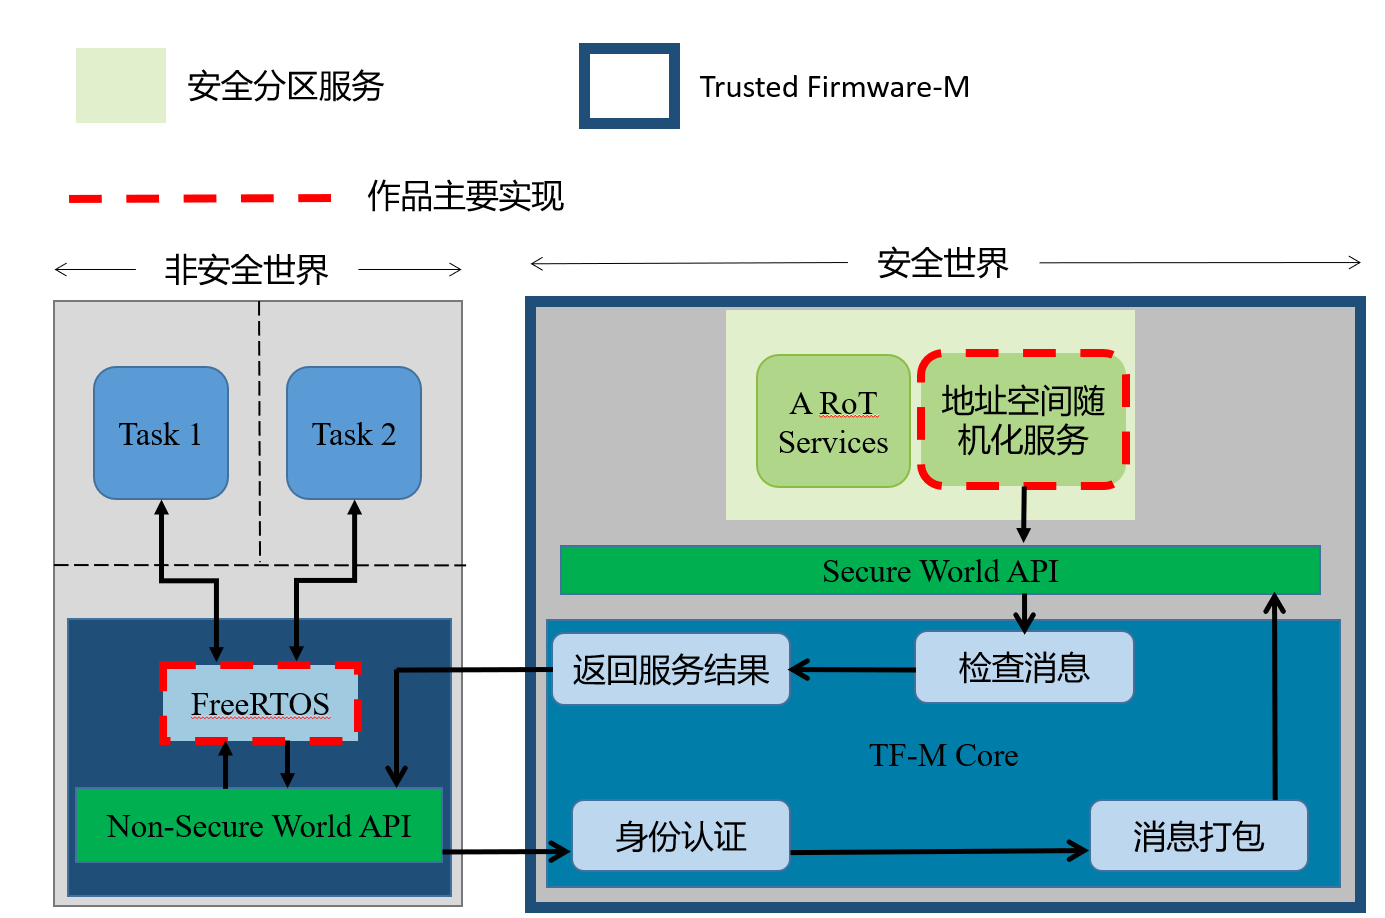
\includegraphics[scale=0.3]{graph/arc.png}
    \caption{系统架构设计}
    \label{fig:system_architecture}
\end{figure}
\par 如图\ref{fig:system_architecture}所示,本作品系统架构设计如下:

\begin{itemize}
    \item \textbf{Trusted Firmware-M(TF-M)框架}:利用Trusted Firmware-M,我们可以为设备的安全性提供一个可靠的基础。这个开源框架提供了一种用于保护设备的方法,包括安全启动,固件更新和安全服务。它也提供了与安全性相关的各种API,让开发人员可以更容易地实现安全功能。
    \item \textbf{函数级地址空间布局随机化服务(ALSR)}:本作品中,我们将函数级地址空间布局随机化服务(ALSR)作为安全服务运行在设备的安全分区中,从而保证其安全性。ALSR服务的主要功能是对设备的固件进行函数级随机化加载,从而防御内存破坏攻击。
    \item \textbf{实时操作系统FreeRTOS}:FreeRTOS是一个小型的实时操作系统内核,我们在非安全世界中运行FreeRTOS并通过函数随机化的安全服务进行重新加载,从而实现对设备的实时调度和安全执行。
\end{itemize}

\subsection{系统实现方案}

\subsubsection{基于 TrustZone-M 的函数级动态随机化加载技术}
\par 本节将会详细阐述基于 TrustZone-M 的函数级地址空间布局随机化技术FASLR的系统设计方案,具体包括:(1)设计静态信息提取机制以对函数函数信息进行收集管理;(2)设计基于 TrustZone-M 的系统安全启动机制以防止代码复用并对函数进行动态劫持;(3)设计函数级随机化加载机制以对函数进行动态随机化加载。随后,针对受限内存场景设计了函数级随机加载内存管理。其中,为对随机化所导致的碎片化内存进行高效管理,实现碎片化内存随机管理机制;为在系统运行时动态获取函数返回信息,实现基于调用栈帧展开的函数完成识别机制;为满足面向受限内存的函数随机化加载以及性能优化,实现基于函数级缓存的内存回收机制。
\paragraph{系统设计}
\subparagraph{系统架构}
\par 本作品的设计基于 TrustZone 的函数级地址空间布局随机化技术 FASLR(Function-based ASLR)。FASLR 的系统架构如图\ref{fig:alsr_architecture}所示,FASLR 由四个主要功能组成部分组成:(i)编译模块(Compile Module,CM),(ii)静态信息提取(Static Information Extraction,SIE),(iii)启动引擎(Boot Engine,BE),以及(iv)函数随机化引擎(Function Randomization Engine,FRE)。
\begin{figure}[H]
    \centering
    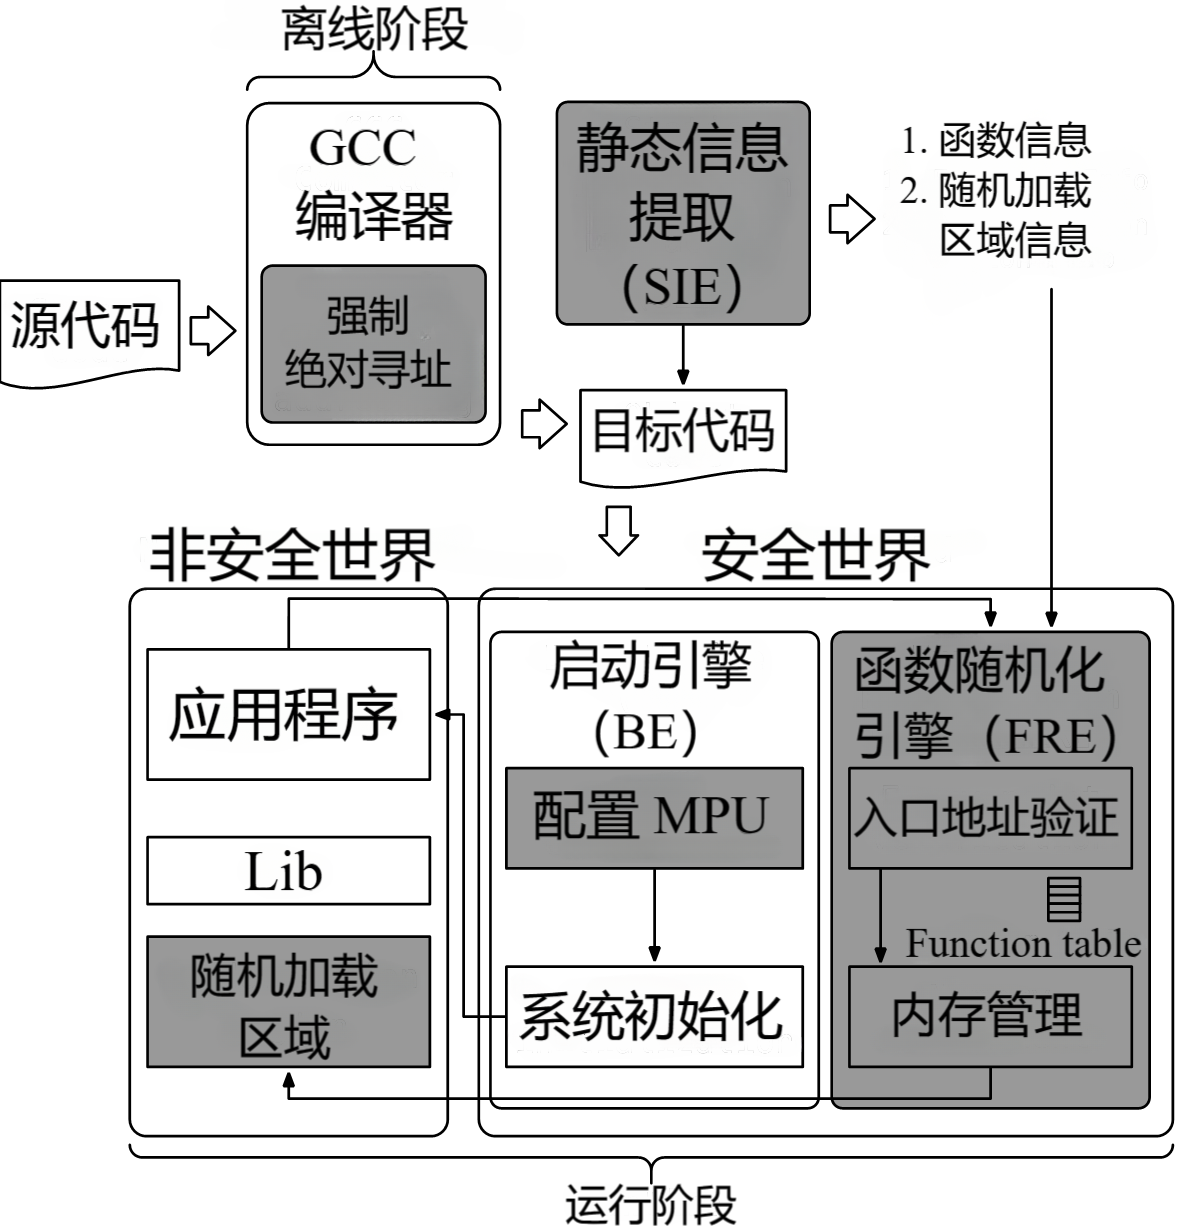
\includegraphics[scale=0.3]{graph/aslr_architecture.png}
    \caption{FASLR架构设计}
    \label{fig:alsr_architecture}
\end{figure}
\par 在离线阶段,FASLR 首先通过 CM 对应用程序进行编译,然后通过 SIE 对编译后的可执行文件进行信息提取,为之后系统运行时对函数进行随机化加载做前期准备。在系统运行阶段,BE 负责对系统进行配置以对应用程序代码进行保护,然后将控制权交给非安全世界的应用程序。最后,在应用程序的运行过程中,由 FRE 负责对其所有函数进行动态的随机化加载。
\par \textbf{编译模块(CM)}:编译模块的目的是使应用程序在函数间调用时采用绝对寻址模式。在 ARMv8-M 架构下,函数间调用可能存在两类寻址模式的跳转指令:绝对寻址模式和间接寻址模式。然而,由于 FASLR 的目标是对应用程序进行以函数为粒度的随机化,每个函数的函数体需要被加载至随机内存地址空间。因此,函数体内部基于相对地址寻址模式指令在随机化后将不再指向原有函数,虽然可以根据随机化信息对此类指令进行运行时重写,但如此做将需要巨大的离线静态分析工作并且严重影响系统性能。为解决上述问题,CM 通过对 GCC 编译器使用特殊的编译标志(-mlong-calls,-fno-jump-tables)对应用程序以及相关库代码进行编译,最终使编译后的可执行文件采用绝对寻址模式。
\par \textbf{静态信息提取(SIE)}:SIE 主要有两个功能:(i)生成 Function Table。当非安全世界代码通过 GCC 编译生成 ELF 格式的目标文件时,SIE 从 ELF 符号表中将所有函数的入口地址以及函数代码大小信息,并且从 .debug\_frame section 中提取函数对应栈帧的大小信息。将每一个函数的上述信息作为表项,全部被存储在称为 Function Table 的数据结构中。(ii)确定随机加载区域。SIE 根据非安全世界应用程序的 ELF 目标文件确定嵌入式设备上空闲 RAM 内存区域,该内存区域在应用程序正常运行时不会被使用。在系统运行阶段,该区域将被 FRE 用于随机化加载函数。
\par \textbf{启动引擎(BE)}:当支持 TrustZone-M 的设备启动时,启动流程按照先后顺序分别是安全世界 Bootloader,安全世界应用程序以及非安全世界应用程序。非安全世界应用程序首先启动 Reset Handler 作为其第一个函数执行。BE 作为安全世界 Bootloader 的一部分存储在安全世界的 Flash 内存。它负责配置内存保护单元(MPU)以使非安全世界代码在 Flash 上不可执行,这样做有两个目的:(i)MPU 保护非安全世界的应用程序以抵御代码复用攻击。(ii)当非安全世界在 Flash 上应用程序被设置为不可执行时,Flash 上任何代码执行会触发 MPU 硬件异常,该异常由安全世界的 HardFault Handler 进行异常处理。
\par \textbf{函数随机化引擎(FRE)}:FRE 作为 HardFault Handler 异常处理的一部分,负责函数的随机化加载,它的主要功能是将被调用的函数加载至随机加载区域并执行该函数。FRE 由函数入口地址验证(Function Entry Point Verification)模块以及内存管理(Memory Management)模块两部分组成。
\par 每当产生 HardFault 异常时,FRE 从异常栈帧中提取当前异常的返回地址(在正常情况下该返回地址为被调用函数的入口地址)。函数入口地址验证负责对该返回地址与 Function Table 中的函数入口地址进行匹配直到匹配成功。这样做有两方面原因,一方面该验证可以判断该异常是否是由正常函数调用所触发。因为有许多情况会引起 HardFault 异常,比如说,攻击者可以通过代码复用攻击执行一条不属于函数入口的指令。因此,该验证可以确保只有当函数入口指令触发异常时才会启动随机化机制。另一方面,通过对 Function Table 中函数入口地址的匹配可以获得该函数的代码大小以及函数栈帧信息,以便后续对其进行随机化加载。
\par 当 FRE 执行完函数入口地址验证后,内存管理模块负责为该被调用函数在随机加载区域随机的分配一块与函数体代码大小一致的 RAM 内存空间并对该函数进行加载(将该函数代码从 Flash 内存复制到已指定的 RAM 内存)。另外,若随机加载区域的 RAM 内存不足则会对已经完成执行的函数进行清理以保证每一次对函数的随机化有足够的内存空间供其被加载。随机加载区域的内存管理在内存受限的场景下具有一定难度,为此本作品设计了一种面向受限内存的函数级随机化内存管理机制并将在作品具体实现章节对其进行具体介绍。函数加载完成后,FRE 恢复该函数的上下文并使其在随机加载区域执行,在该过程中,本作品需要维护非安全应用程序的控制流以及其处理器模式以保证其正常运行。然而,函数随机化后,当前的控制流处于 HardFault 异常处理状态中,因此,本作品需要将控制流从异常处理状态转移至随机加载区域的被调用函数。尽管可以使用跳转指令直接从异常处理跳转至随机加载区域的函数入口,但该操作会破坏函数原有的调用栈从而导致函数的上下文不一致。另外,在 ARMv8-M 架构下,处理器在异常处理时总是处于 handler 模式,且其访问级别为特权态,因此直接使用跳转指令从异常处理机制恢复原来的处理器模式,可能使被调用函数的处理器模式前后不一致且存在越权的安全隐患。为解决上述问题,本作品对异常栈帧进行重写,修改其中的返回地址为被调用函数在随机加载区域的函数入口地址。至此,当异常处理机制执行返回操作时,硬件将异常栈帧中保存的上下文信息进行恢复,并且将异常栈帧中的异常返回地址(即被调用函数在随机加载区域的函数入口地址)赋于处理器的 PC 寄存器。因此在下一个处理器时钟周期处理器将返回至随机加载区域并重新执行被调用函数,同时,处理器模式也恢复为触发异常前的状态。

\subparagraph{工作流程}
\par 离线阶段:离现阶段主要负责代码编译以及烧录。在 GCC 编译器编译和链接非安全世界应用程序时,SIE 根据其 ELF 目标文件生成 Function Table。Function Table、BE 以及 FRE 被烧录至安全世界的 Flash 内存,而非安全世界应用程序的固件则被烧录至非安全世界的 Flash 内存。
\par 运行阶段:部署 FASLR 的系统运行时,所有对 Flash 内存上函数的调用都会将该函数加载至随机加载区域并执行。具体来说,当系统运行过程中一旦有产生函数调用,系统会跳转至被调用函数 callee 进行执行,由于 callee 对应的代码存储在 MPU 所保护的 Flash 内存上,因此系统尝试执行 callee 代码时将会触发 MPU 异常处理。此时,FRE 在 MPU 异常处理中对 callee 进行随机化加载,然后将控制流从 callee 在 Flash 内存的代码转移到该函数在随机加载区域的代码并恢复 callee 的执行。类似的,在 callee 的执行过程中,由于所有 callee 产生的函数调用依然指向 Flash 内存的函数代码,因此同样会触发 FRE 对其进行随机化加载至随机加载区域并执行。在函数执行完成后,函数将会返回至随机加载区域,并继续执行其被调用位置的下一条指令。FRE 通过上述方式对所有指向 Flash 内存的函数调用进行随机化并保证函数的正常执行。
\par 设备上电后,安全世界的 BE 对 MPU 进行相关配置然后启动非安全世界程序的 Reset Handler。Reset Handler 执行一系列的初始化操作后将会执行非安全世界的 main 函数,其中,Reset Handler 和 main 函数都会触发函数随机化加载,两个函数的函数体代码都会被 FRE 随机化加载至 RAM 内存中的随机加载区域中并执行。同样的,在 main 函数的执行过程中,一旦 main 函数中产生对 Flash 内存上函数的调用,控制流会被 FRE 所截获并对该函数进行随机化加载然后在随机加载区域恢复该函数的执行。以此类推,所有的函数都会被加载至随机随机加载区域执行。
\par 图\ref{fig:workflow}为程序在部署FASLR情况下的系统进行函数调用时的工作流程示意图,该图展示了函数X、Y、Z之间的调用过程,调用顺序为X调用Y,Y调用Z,图中$X^{'}、Y^{'}、Z^{'}$分别对应函数X、Y、Z在随机加载区域的函数体。该流程图包括运行过程中的函数调用(\ding{172}和\ding{175})、MPU异常处理(\ding{173}和\ding{176})、运行时函数随机化、函数执行(\ding{174}和\ding{177})以及函数返回(\ding{178}和\ding{179})。该流程图假设函数X已被加载进随机加载区域并从函数$X^{'}$开始执行,当$X^{'}$调用Y时(\ding{172})将会导致MPU异常(\ding{173})并触发HardFault Handler中的FRE。然后FRE将Y加载至随机加载区域并将控制流转移给$Y^{'}$(\ding{174})。在$Y^{'}$的执行过程中,$Y^{'}$将会调用Y,MPU异常再次被触发(\ding{175})并交给FRE进行处理(\ding{176}),控制流再次转移至$Z^{'}$。当$Z^{'}$执行完成后,控制流将会从$Z^{'}$返回至$Y^{'}$,再由返回至$X^{'}$。
\begin{figure}[H]
    \centering
    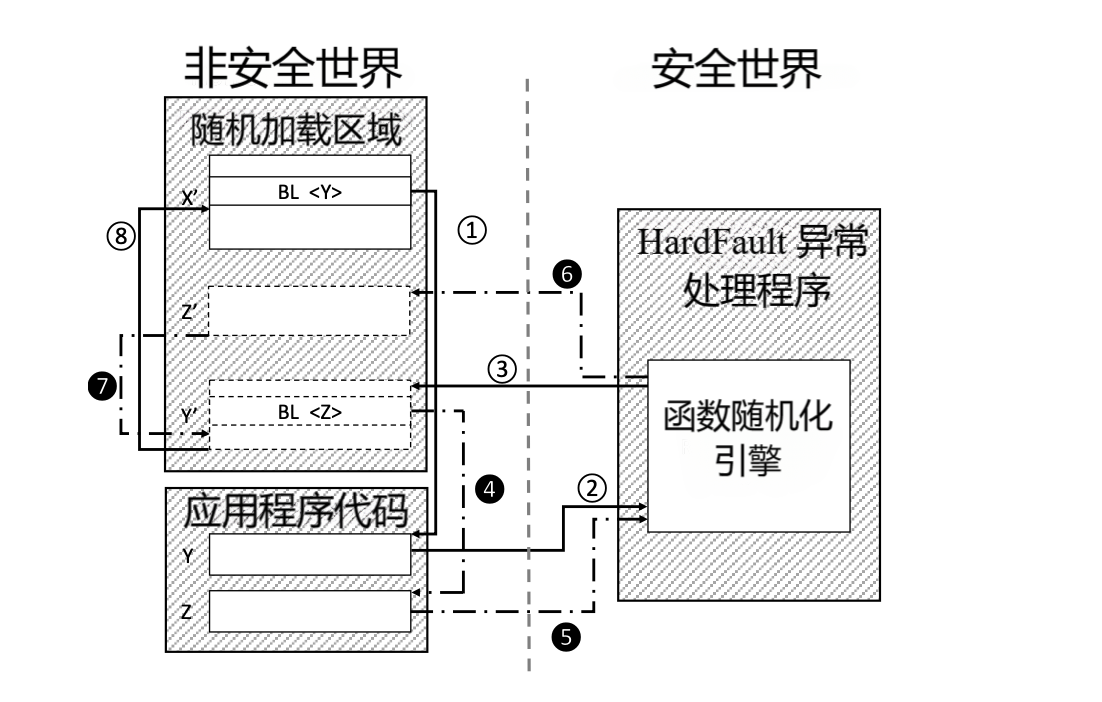
\includegraphics[scale=0.35]{graph/workflow.png}
    \caption{FASLR系统工作流程}
    \label{fig:workflow}
\end{figure}
\paragraph{面向受限内存的函数级随机化内存管理}
\par 与通用系统的内存管理一样,针对随机加载区域的内存管理不仅决定系统能否正常运行,而且对系统性能起着关键性影响。面向受限内存的函数级随机化内存管理的设计目标是在受限内存场景下,为能够随机化加载函数,实现高效的内存分配以及回收机制,保证系统可以正常运行并尽量不影响系统性能。
\par 通常来说,内存管理机制会对空闲内存进行地址连续的空间分配。但在需要对函数进行随机化加载的场景下,为保证分配内存的地址随机性,内存将会被切割成大小不一的不连续地址块,最终导致内存碎片化(Memory Fragmentation)。为实现对碎片化内存的高效管理,本作品设计了一种碎片化内存随机管理机制。
\par 尽管碎片化内存随机管理机制负责对内存进行回收,但如何选取回收内存的对象以及回收的时机至关重要。这一点决定了系统是否能够存在足够的内存以对函数进行随机化加载。具体来说,针对内存受限的低端嵌入式设备,在函数加载过程中可能会出现内存不足的情况,即其随机加载区域内存大小可能不足以加载整个非安全世界应用程序代码并执行。因此,需要对已加载的函数进行内存回收,以确保有足够的内存分配给当前函数。然而,由于函数与函数之间具有关联性,随意对已加载的函数进行内存回收将会影响程序正常执行。例如存在若干函数未完成执行,这些函数可能调用了其他函数且该被调用函数未返回,一旦将此类函数的内存进行回收,那么当其调用函数返回时,其返回地址则是无效地址,最终导致不可预测的结果。因此,在回收前需对已加载函数进行筛选,识别已完成的函数并对其进行回收。然而,由于FASLR在系统运行时无法动态获取函数返回信息,识别已完成函数具有一定难度。为此,本作品设计了一种基于调用栈帧展开的函数完成识别机制。
\par 另一方面,由于内存回收具有一定的性能开销,选择合适的时机对内存回收不仅能够保证有足够内存用于函数加载,而且能减少内存回收次数从而降低系统的性能开销。此外,由于低端嵌入式系统中存在大量循环,循环内的函数会被不断调用。然而,对于未被回收内存的函数,任何对该函数的重复调用依然会触发异常从而导致FRE的随机化加载,频繁的函数加载会严重影响系统性能。为此,本作品设计了一种基于函数级缓存的内存回收机制,通过函数级缓存以提高内存利用率并减少函数加载次数。为减少内存回收次数,实现在合适时机对函数内存进行回收;为减少函数的重复加载,实现对已加载函数调用机制的优化。
\subparagraph{碎片化内存随机管理}
\par 内存管理的关键是要将随机加载区域的已用内存和空闲内存的边界进行统一高效的管理。碎片化内存随机管理机制的基本思路是将内存以块链表进行管理,以内存块的形式为函数分配大小匹配的内存。具体地,本作品采用显式空闲块链表(Implicit Free Lists)的方式对内存块进行管理。内存块的数据结构如图\ref{fig:memoryManagement}(a)所示,主要包括元数据、负载数据以及填充数据:元数据由内存块的大小、以及指向下一个内存块的指针组成;负载数据用于对函数代码的加载;填充数据用于内存对齐。为方便叙述,本作品将已加载的函数所占有的内存块称为函数块,而其余的内存块则称为空闲块。本节从内存分配以及内存回收两方面对碎片化内存随机管理机制进行详细介绍。
\begin{figure}
    \centering
    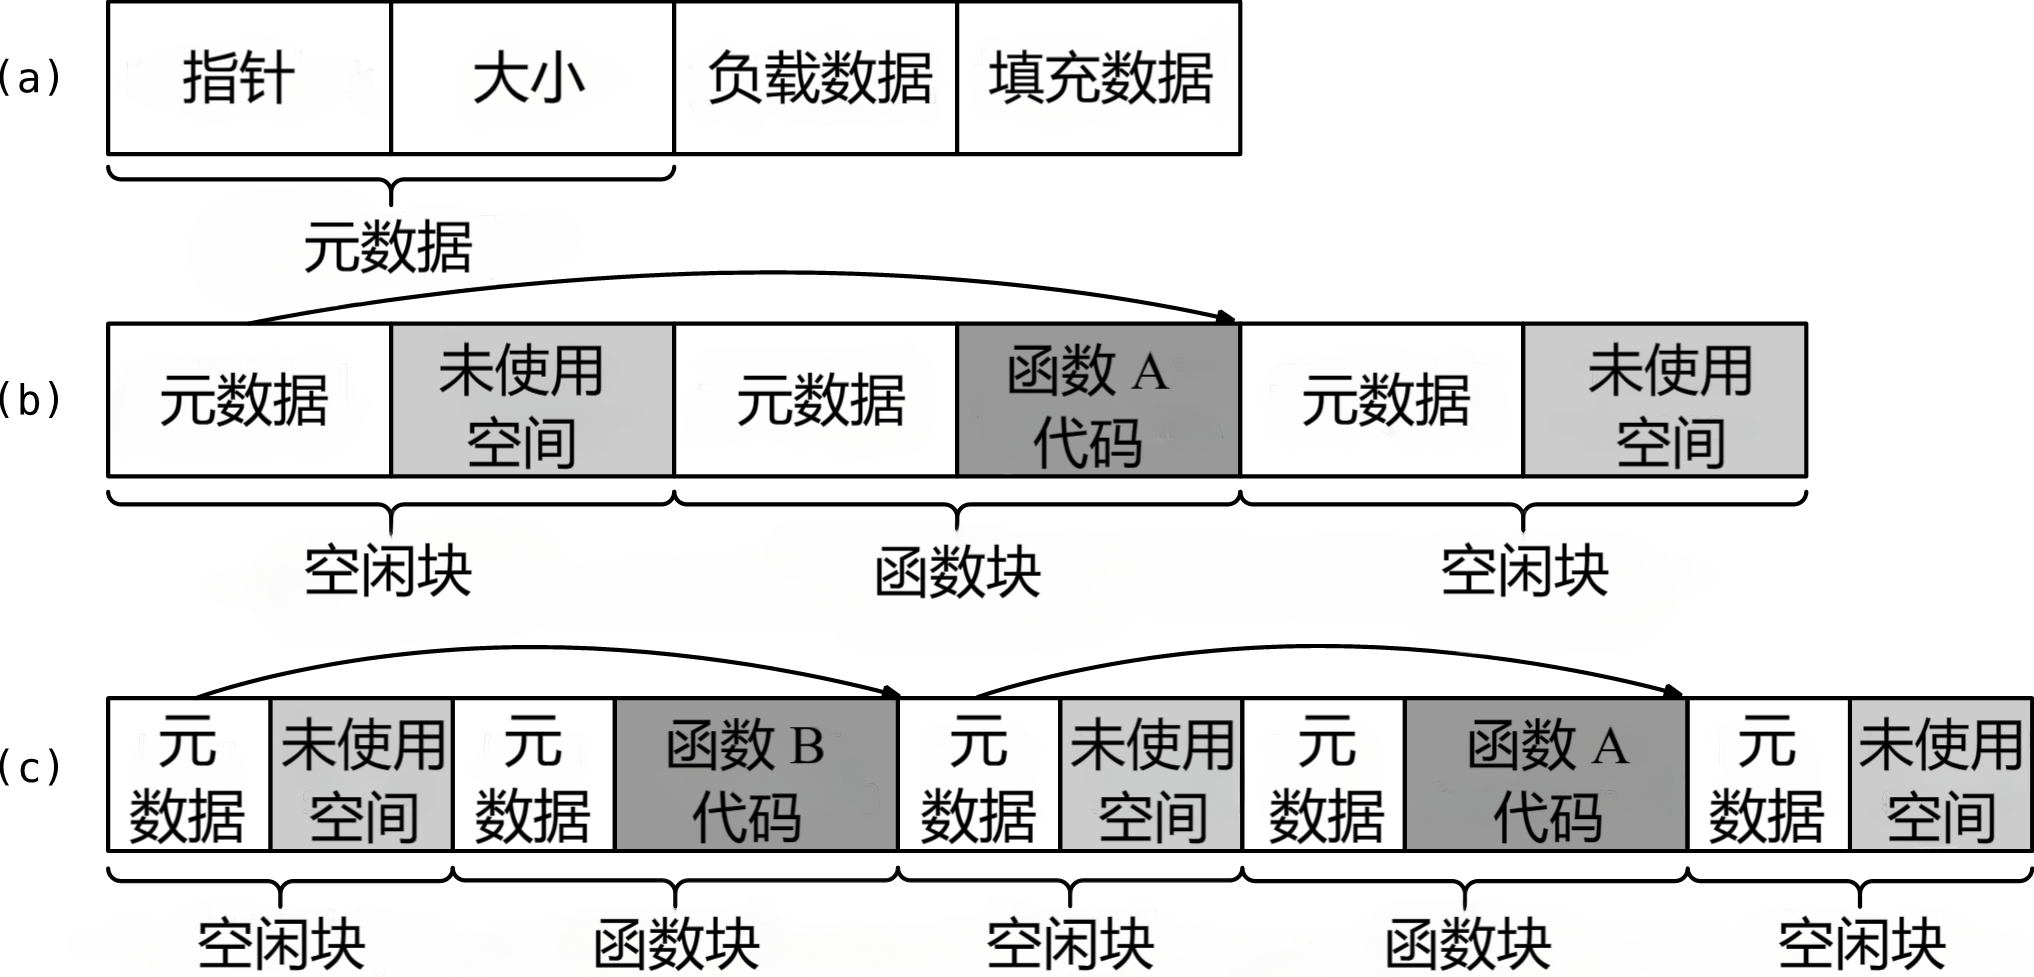
\includegraphics[scale=0.23]{graph/memoryManagement.png}
    \caption{基于显式空闲链表的内存管理}
    \label{fig:memoryManagement}
\end{figure}
\par 当系统启动时,FRE首先将整个随机加载区域初始化成一整个空闲块,加载若干函数后,该空闲块会形成一个空闲块链表。具体来说,当有函数需要被加载时,其函数体大小为$S_f$​,FRE首先扫描空闲块链表直到找到符合该函数体大小的空闲块,该内存块大小$S_b$​满足:
\begin{equation}
    S_b-S_{meta}≥S_f \label{1}
\end{equation}
\par 其中,$S_{meta}$表示元数据的大小。获得内存块以后,FRE从中随机的选取一个空闲块。由于用于函数加载的内存可能只占空闲块内存的部分,为了更高效的利用其余内存,FRE通过判断该内存块是否可以分裂成三个块:一块函数块以及两块空闲块。符合该条件的内存块大小应当满足:
\begin{equation}
    S_b-3*S_{meta}≥S_f
\end{equation}
\par 对于不满足该条件的空闲块,直接返回其负载数据段的起始地址作为内存分配的地址。对于符合该条件的空闲块,则从该空闲块的负载数据段再次随机选取内存地址用于函数加载,最终由公式(3)得到内存分配地址address。同时,FRE根据该地址构建一个函数块,并对其余空闲内存构建两个空闲块插入原空闲块链表。举例来说,图\ref{fig:memoryManagement}(b)表示在FRE在加载函数B前随机加载区域内存的状态,在当前情况下,函数A已被加载,且与其相邻的存在两个空闲块。当FRE加载函数B后,如图\ref{fig:memoryManagement}(c)所示,函数块A左侧的空闲块分裂成三个部分,包括一个存放函数B代码的函数块及其相邻的空闲块。
\begin{equation}
    address=ranom\%(S_b-3*S_{meta}-S_f)
\end{equation}
\par 内存的回收过程是将函数块插入空闲块链表的过程。具体地,FRE根据函数块的地址位置,扫描空闲块链表直到找到其在空闲块链表中对应插入位置。在插入过程中,FRE先判断该函数块是否能与其前一个空闲块或者后一个空闲块合并,最终合成新的空闲块链表。
\subparagraph{基于调用栈帧展开的函数完成识别}
\par 基于调用栈帧展开的函数完成识别机制的目标在于从当前所有已加载的函数识别出已完成执行的函数。对于当前正在执行的函数来说,本作品将其直接调用者及其间接调用者称为祖先函数(Ancestor Function)。在系统运行过程中,当前正在执行函数的祖先函数通常在等待其调用函数的返回,因此,此类函数的内存空间不能回收。除了当前正在执行的函数及其祖先函数,随机加载区域内其他已加载的函数称为已完成函数(Finished Function)。为识别已完成函数,本作品的基本思路是对所有已加载函数进行记录,然后根据当前调用栈信息识别出当前执行函数的所有祖先函数,最后从已加载函数中过滤所有祖先函数从而得到全部已完成函数。
\begin{figure}[H]
    \centering
    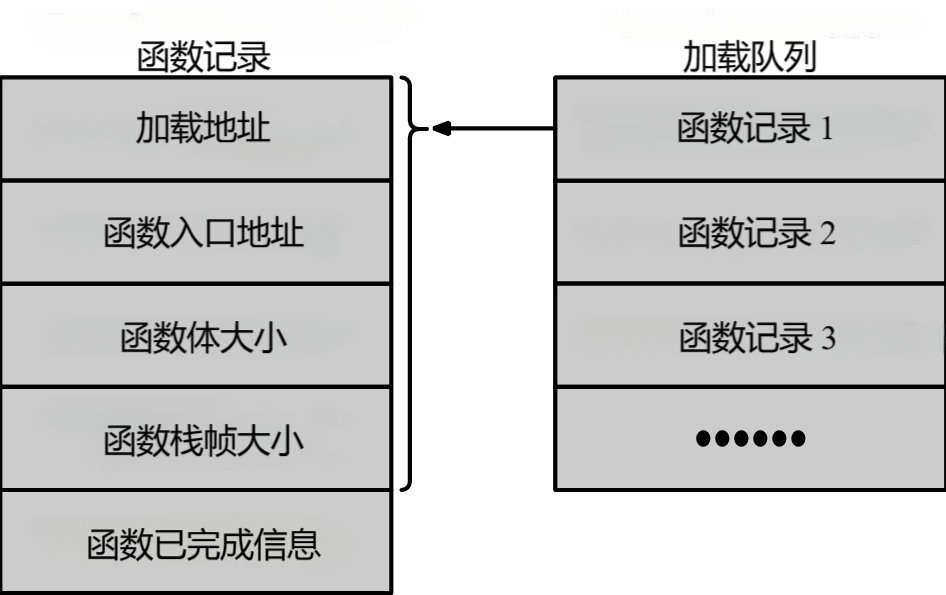
\includegraphics[scale=0.45]{graph/dataStructure.png}
    \caption{函数记录以及加载队列的数据结构}
    \label{fig:dataStructure}
\end{figure}
\par 具体地,FRE在每一次函数加载时会对该函数信息进行记录,用于表示函数信息的数据结构称为函数记录(Function Record)。如图\ref{fig:dataStructure}所示,一个函数记录包括:(i)该函数在随机加载区域的函数入口地址,(ii)该函数体的大小,(iii)函数栈帧大小,(iv)该函数已完成信息,(v)函数原始入口地址。其中,函数入口地址与函数体大小决定了该函数的加载区域范围,函数栈帧大小表示其在执行的时候所需要栈的大小,函数已完成信息表示该函数是否已完成执行,函数原始入口地址表示该函数在Flash内存中的入口地址。为对所有已加载函数进行记录,FRE用一个称为加载队列(Loading Queue)的数据结构以存储所有函数记录。
\par 调用栈通常被用于追踪函数执行流,在ARMv8-M架构中,一般情况下最先被压入函数栈帧的是函数的返回地址。因此,一旦确定了函数的栈帧,其栈帧最底部存放的值则是该函数的返回地址,从而根据函数记录的加载区域与该返回地址进行匹配以最终确定该函数的调用函数。FRE根据调用栈中存放的函数返回地址,在加载队列的函数记录中不断回溯其调用函数直到找到所有祖先函数,并对这些祖先函数对应的函数记录进行标记。
\begin{figure}[H]
    \centering
    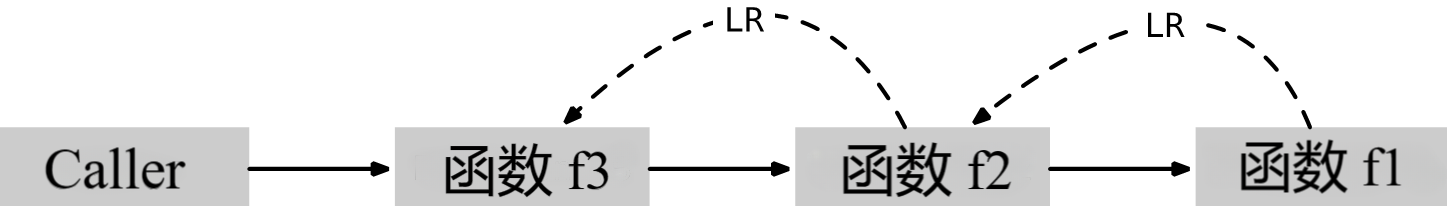
\includegraphics[scale=0.3]{graph/funcCall.png}
    \caption{f3、f2以及f1的函数调用关系}
    \label{fig:funcCall}
\end{figure}
\par 具体而言,在如图\ref{fig:funcCall}所示的调用过程中,其调用栈帧图如图\ref{fig:stackFrame}所示,当函数$f_0$被调用从而触发HardFault异常处理时,硬件自动将产生异常前的上下文信息通过异常栈帧保存,异常栈帧有固定大小$s_e$。FRE通过读取非安全世界的栈指针寄存器获得当前应用程序的栈指针SP并通过异常栈帧获得当前函数的返回地址$R_0$。此时,由于当前函数未被执行,栈上的第一个函数栈帧属于当前函数的调用函数$f_1$,其栈帧顶部地址$T_1=SP+s_e$。为获取$f_1$的调用函数,则需要获取其栈帧大小从而得到其函数返回地址,因此FRE需要定位$f_1$对应的函数记录。它对加载队列中的函数记录进行扫描直到$R_0$恰在某一函数记录对应的加载区域内,则该函数记录所对应的函数即为$f_1$。然后,FRE根据$f_1$的栈帧大小$s_1$可以确定$f_1$的调用函数$f_2$的栈帧顶部地址$T_2=T_1+s_1$。由于$f_1$的返回地址存放在其栈帧底部,即与$f_2$栈帧顶部$T_2$相邻,因此通过$T_2$可以得到$f_1$的返回地址$R_1$。同样的,根据$R_1$和$T_2$可以从加载队列中得到$f_2$的函数记录、$T_3$以及$f_2$的返回地址$R_2$。重复上述过程,FRE可以根据调用栈帧展开得到当前函数的所有祖先函数$f_1、f_2、f_3……f_n$,并在加载队列中对其函数记录标记为已完成。
\subparagraph{基于函数级缓存的内存回收}
\par 基于函数级缓存的内存回收机制的目标是提高随机加载区域内存利用率以优化系统性能。其基本思路是尽可能的将已加载函数放置在随机加载区域,将其作为FRE函数加载时的函数级“缓存”。
\begin{figure}[H]
    \centering
    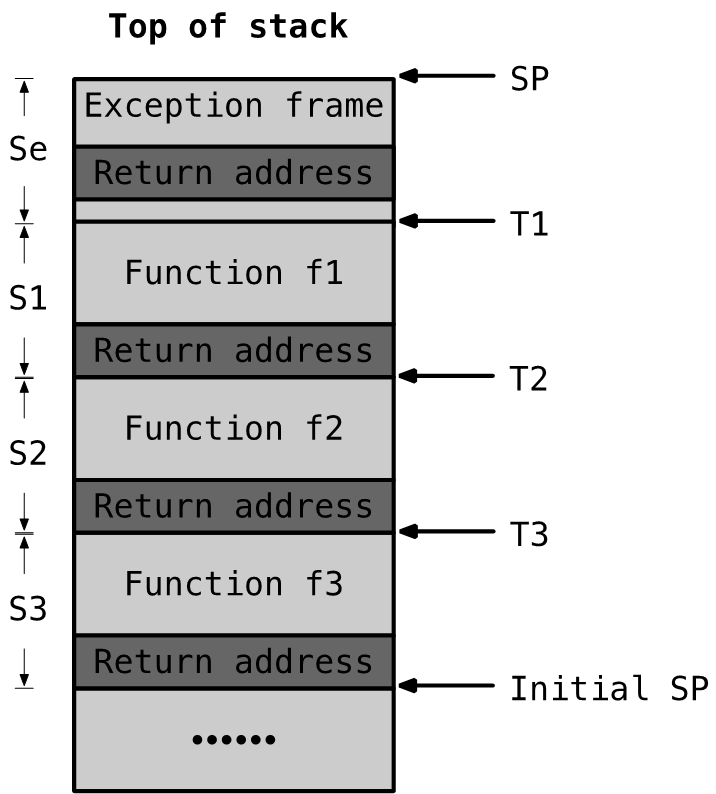
\includegraphics[scale=0.4]{graph/stackFrame.png}
    \caption{函数调用栈帧结构}
    \label{fig:stackFrame}
\end{figure}
\par 具体地,FRE使用函数记录保存已加载函数信息,并将其放入加载队列,该加载队列即为函数缓存。当FRE对当前函数进行加载时,它首先通过异常栈帧获得函数的原始入口地址,随后通过该地址与加载队列中的函数记录进行匹配,从而判断该函数是否已存在缓存中。若是,则称为函数缓存命中(Function Cache Hit),此情况下FRE不再对该函数进行随机化加载,而是直接根据函数记录得到该函数在随机加载区域的函数入口地址并恢复该函数的执行。若不是,则称为函数缓存缺失(Function Cache Miss),此情况下FRE按照原执行流程对该函数进行随机化加载。在函数级缓存基础上,为进一步减少函数加载次数,提升系统性能,本作品设计了函数调用重定向以及函数内存按需清理。
\par 函数调用重定向:函数调用重定向是通过优化重复函数调用以减少重复的函数加载。其基本思路是针对当前已被加载的函数,对其被调用点(即该函数的调用函数调用该函数的指令所在位置)对应的函数入口地址值进行重写,使该函数调用所指向的函数入口地址由该函数在Flash上的对应地址变为在随机加载区域的对应地址。具体地,当函数调用触发FRE的随机加载机制时,FRE会判断该函数是否已在函数缓存中,若是,则说明该函数目前正在被重复加载。因此,FRE通过异常栈帧找到该函数的返回地址,并由此找到该函数的被调用点并对该调用点对应的函数入口地址值进行重写使其指向该函数在随机加载区域的函数入口地址。至此,下一次对该函数的调用则会直接跳转至随机加载区域而不触发FRE。举例来说,如\ref{fig:redirection}所示,在系统运行过程中函数A将会重复调用函数B,函数B在随机加载区域的加载地址为0x20002c00,在未进行函数调用重定向时,函数A每次对函数B的调用都将会触发MPU异常并经由FRE对其进行加载并执行。在启用函数调用重定向的FASLR情况下,在函数A第二次调用函数B时,FRE根据函数的函数入口地址查找发现函数B的函数记录已存在函数缓存中,随后FRE根据异常栈帧中LR寄存器的值以获得函数A调用函数B的指令位置,即blx指令的下一个指令所在的地址,FRE对该blx指令的机器码进行解码得到其跳转寄存器为R3,然后FRE向上遍历寻找对R3的赋值指令(图\ref{fig:redirection}中的movw以及movt指令)并对其进行重新编码以将其跳转地址改为函数B在随机加载区域的加载地址,修改完成后,函数A对函数B的调用将会被直接重定向至随机加载区域而不再触发MPU异常,从而大大减少了异常触发的频率,极大减少了其所带来的性能开销。
\begin{figure}[H]
    \centering
    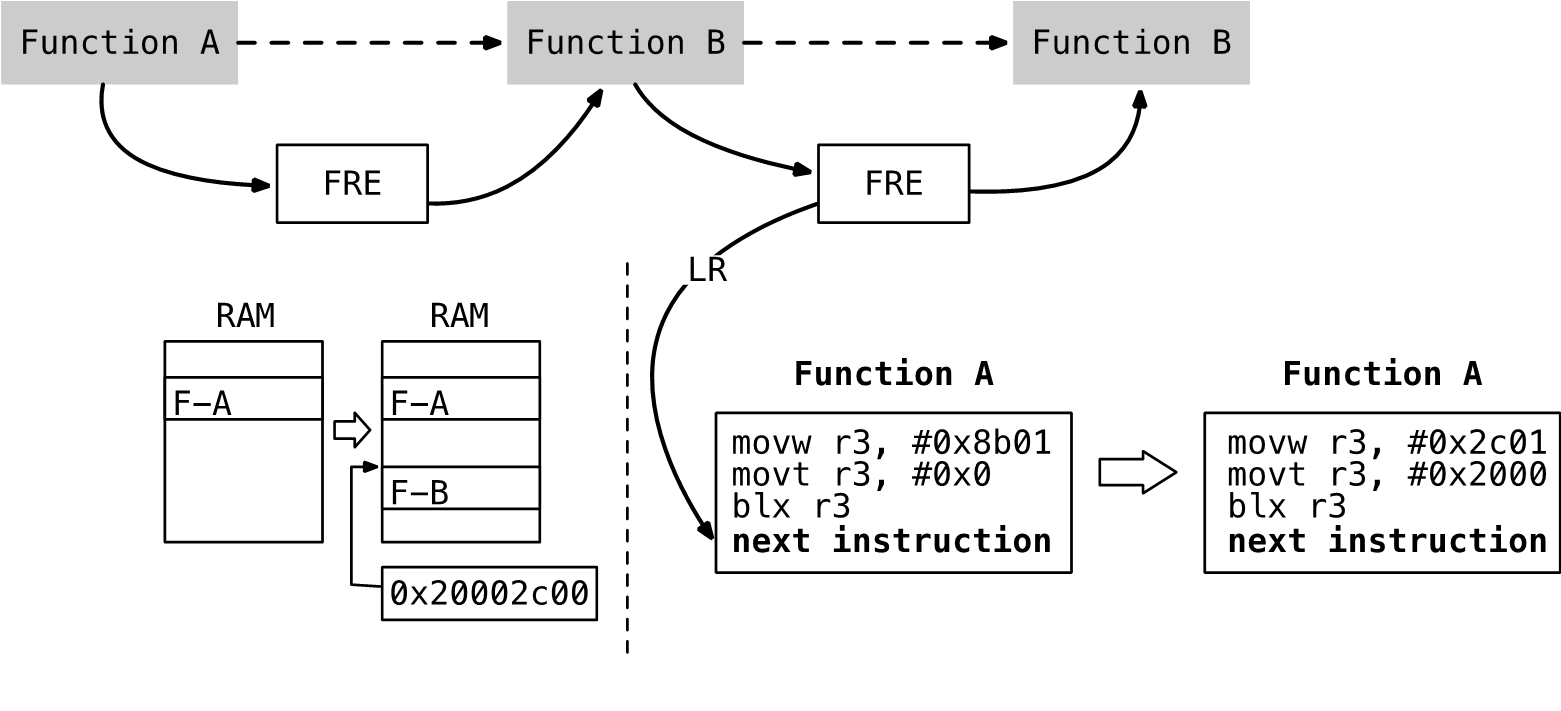
\includegraphics[scale=0.5]{graph/redirection.png}
    \caption{函数调用重定向}
    \label{fig:redirection}
\end{figure}
\par 此外,由于FRE可能随时对某个函数内存进行回收,对该函数的被调用点进行重写则会使下一次调用该函数时跳转至无效的函数入口,从而导致意想不到的后果。因此,FRE构建一个重写链表(Rewriting List)用于统一保存所有重写的信息(重写的位置及其原值),并在函数内存回收前根据该重写链表对重写过的调用点进行还原。
\par 函数内存按需清理:函数内存按需清理是为保证在有足够内存用于函数随机化加载的情况下尽可能减少内存回收的次数,通过提高函数缓存利用率以减少函数加载次数,FRE仅在当前随机加载区域内存不足以加载当前函数时才会执行内存回收。在对函数进行随机化加载前,FRE首先检查是否有足够内存加载该函数。若没有,FRE会根据重写链表还原被重写的调用点,然后利用基于栈的函数完成识别机制在函数缓存(即加载队列)中对所有已完成函数进行标记,最后将函数缓存中所有标记的函数执行内存回收并更新函数缓存。

\paragraph{函数信息自动化提取工具ELF-To-FUNCS}
\subparagraph{ELF-To-FUNCS的简介}
\par 为提高工程效率,减少人工出错的可能性,我们编写了函数信息自动化提取工具ELF-To-FUNCS。本工具利用Python以及第三方库pyelftools对elf文件进行解析,并且对相应的函数信息进行提取。同时,利用提取的信息修改Function table。
\par 由于本工具基于跨平台编程语言Python,因此不受不同操作系统和不同环境的约束,部署简单,可移植性高。
\subparagraph{ELF-To-FUNCS的实现}
\par ELF (Executable and Linking Format)指可执行和可链接格式,最初是由UNIX系统实验室(USL)开发和发布的,作为应用程序二进制接口(ABI)的一部分。现在Linux、FreeBSD、macOS等许多操作系统中都有广泛的应用。参照TIS协会制定的elf标准文档1.2版本,可知elf文件主要由图\ref{elf}所示的几个部分构成。其中,在Sections中存在.symtab节和.debug节。在.symtab节中包含符号表(Symbol Table),在debug节中保存有关符号调试的信息。
\begin{figure}[H]
    \centering
    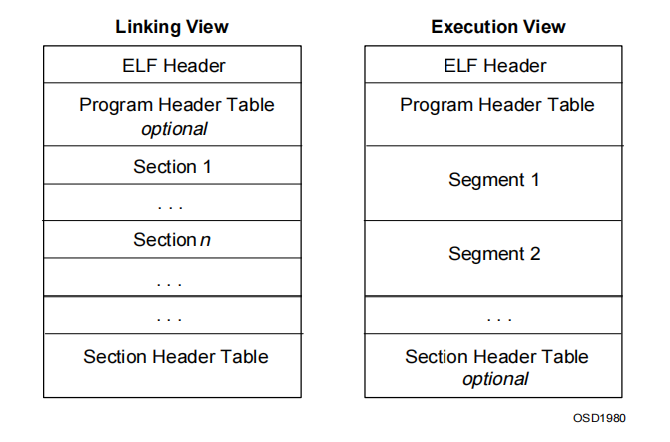
\includegraphics[scale=1.2]{graph/elf_struct.png}
    \caption{ELF结构图}
    \label{elf}
\end{figure}
\par 如图\ref{sf},在符号表中包含了STT\_FUNC符号,该符号与一个函数或其他可执行代码相关联。
\begin{figure}[H]
    \centering
    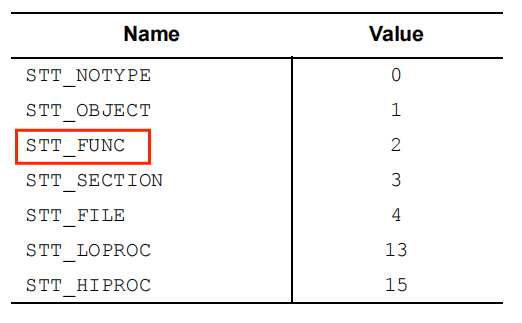
\includegraphics[scale=1.2]{graph/stt_func.png}
    \caption{符号表部分结构图}
    \label{sf}
\end{figure}
\par 并且基于符号表的结构:
% \begin{verbatim}
%     typedef struct { 
% Elf32_Word st_name; 
% Elf32_Addr st_value; 
% Elf32_Word st_size; 
% unsigned char st_info; 
% unsigned char st_other; 
% Elf32_Half st_shndx; 
% } Elf32_Sym;
% \end{verbatim}
\begin{lstlisting}[language=C]
typedef struct { 
    Elf32_Word st_name; 
    Elf32_Addr st_value; 
    Elf32_Word st_size; 
    unsigned char st_info; 
    unsigned char st_other; 
    Elf32_Half st_shndx; 
} Elf32_Sym;
\end{lstlisting}
\par 我们就可以通过提取elf的符号表中的STT\_FUNC符号来获取函数信息,然而,对于不同的操作系统,其对elf解析的实现有所不同,因此我们采用跨平台编程语言Python作为开发工具,具体的,我们利用pyelftools中的dwarfinfo模块,获取sections中的符号表,定位到STT\_FUNC符号,找到对应的函数信息,进行提取保存。
\par 同时,在本作品的elf文件中存在.debug\_frame节,debug\_frame是一种调试信息,它是用于支持栈回溯的一种数据结构。在程序崩溃或者出现异常时,栈回溯是一种快速诊断和解决问题的方法。由于程序在运行时会使用堆栈来保存临时变量和函数调用信息,因此栈回溯需要了解每个被调用函数的参数、返回地址和局部变量等信息。这些信息都保存在debug\_frame中。debug\_frame通常由两个部分组成:FDEs(Frame Description Entries)和CIEs(Common Information Entries)。CIEs包含了所有与堆栈回溯相关的通用信息,比如访问寄存器的方式、数据类型、偏移量等等。一个CIE可以对应多个FDE。FDEs包含了与具体函数相关的信息,如该函数在代码段中的起始和结束地址、stack frame layout等,它们可以通过CIEs进行索引查找。如果找到了函数对应的FDES就可以获取其起始地址,对Function table进行修改。
% \begin{figure}
%     \centering
%     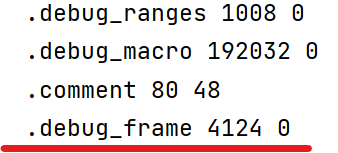
\includegraphics[scale=1]{graph/debug_frame.png}
%     \caption{.debug节内容}
%     \label{df}
% \end{figure}
\par 具体的,我们利用pyelftools中的callframe模块,提取CIE和FDE信息,如图\ref{id}的‘initial\_location’即为函数首地址。
\begin{figure}[H]
    \centering
    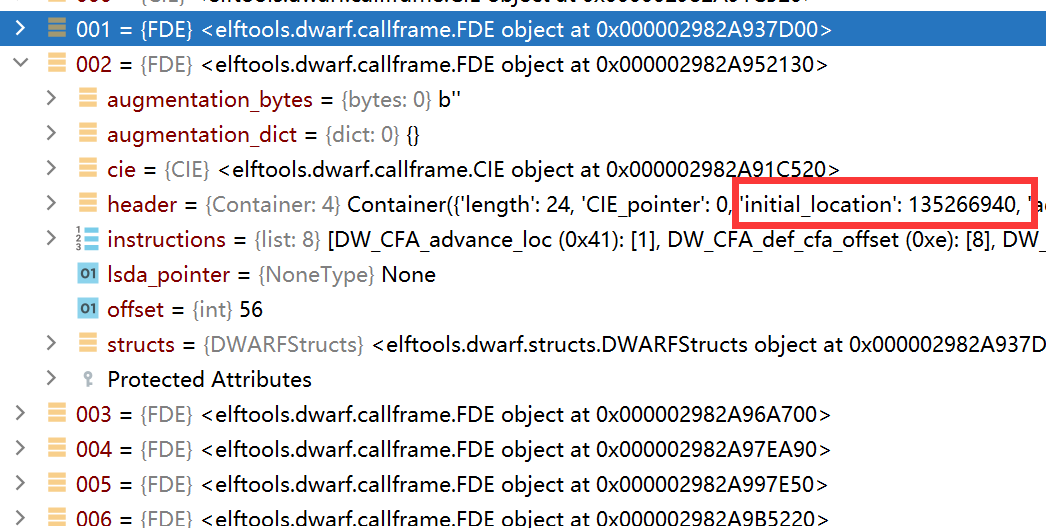
\includegraphics[scale=0.3]{graph/A.png}
    \caption{FDE对应首地址}
    \label{id}
\end{figure}
\par 通过上述工作,我们最终工具整合成以下结构:
\begin{itemize}
    \item config.ini:配置文件,包含重要文件的路径。
    \item ELF\_frames\_sizes.txt:用于保存提取出的函数地址以及调用帧大小信息。
    \item funcs.txt:用于保存从elf文件中提取出的函数信息。
    \item funcs\_sizes.txt:用于保存包含调用帧大小的函数信息。
    \item funcs.c: 样例文件,本文件为函数列表的样例。
    \item frame\_parser.py: 框架解析文件,本文件用于解析elf文件,获取相应信息。
    \item main.py: 本文件用于修改`func.c`文件。
    \item tutorial.md: 本工具的使用教程。
\end{itemize}
\par 在使用前只需要填写config.ini的elf文件的路径<Elfpath>和需要修改的函数表的路径<func.c Path>即可,实现对函数信息的自动化修改。



\subparagraph{ELF-To-FUNCS的优势}
\begin{itemize}
    \item 自动化操作:本工具可以自动地完成函数表的修改,从而减少了人工操作。在传统的手动修改中,需要对每个函数表项进行逐一修改,容易出现疏漏或者错误。而本工具可以自动化地完成这个过程,减少了出错的可能性,同时也提高了开发效率。
    \item 精确性高:本工具利用 ELF 文件格式规范来定位和操作函数表,避免了手动修改过程中可能出现的错误。手动修改时,可能会误操作或者定位不准确,从而影响程序的正确性和稳定性。本工具利用了文件格式规范,能够精确地定位和操作函数表,从而保证了修改的准确性和稳定性。
    \item 良好的可移植性:本工具使用跨平台编程语言Python作为开发工具,并利用其提供的第三方库pyelftools。在不同系统或者环境下都能够良好地运行,不需要对代码进行大量修改或者适配。这使得部署变得更加简单,并且提高了代码的可移植性和灵活性。
    \item 可扩展性好:本工具采用了良好的软件工程实践,可以根据需要进行修改和定制,以满足不同应用场景下的需求。工具中的代码结构清晰,函数模块化,易于阅读和维护。这意味着可以在需要的情况下轻松地扩展新的功能或者修改现有的功能,从而使工具更加适合不同的使用情境。
\end{itemize}

\subparagraph{ELF-To-FUNCS的应用场景}
\par ELF-To-FUNCS主要应用于软件开发和维护领域,除了本作品中用于嵌入式开发,自动修改其函数信息。使用本工具还可以定位到需要修改的函数表,并修改其中相应函数的指针。除此之外,在软件升级过程中,需要更新旧版本中的某些函数。使用本工具可以方便地解析 ELF 文件,定位到函数表所在的段,并修改其中的函数指针,实现函数替换操作。并且在软件逆向工程或者漏洞挖掘过程中,需要对 ELF 文件进行修改以绕过某些安全检测或者实现某些攻击。使用本工具可以快速定位到需要修改的函数表,插入指定的函数指针,从而达到相应的目的。
综上,本工具可以广泛应用于软件开发和维护领域,能够为开发人员提供便利,降低出错的可能性,并且增强了软件开发和维护的效率。
\subparagraph{ELF-To-FUNCS的应用实例}
\par 现给出具体实例展示本工具的使用流程及其可行性。
\begin{enumerate}
    \item 填充配置文件。
          \begin{enumerate}
              \item 如图\ref{gl},将待解析的elf文件路径填入<Elfpath>,本例改为\begin{verbatim}C:\Users\Robin\Desktop\GPIO_IOToggle_TrustZone_NonSecure.elf\end{verbatim},将需要修改的函数表路径写入<func.c path>,本例为\begin{verbatim}C:\Users\Robin\Desktop\funcs.c\end{verbatim}
                    \begin{figure}[H]
                        \centering
                        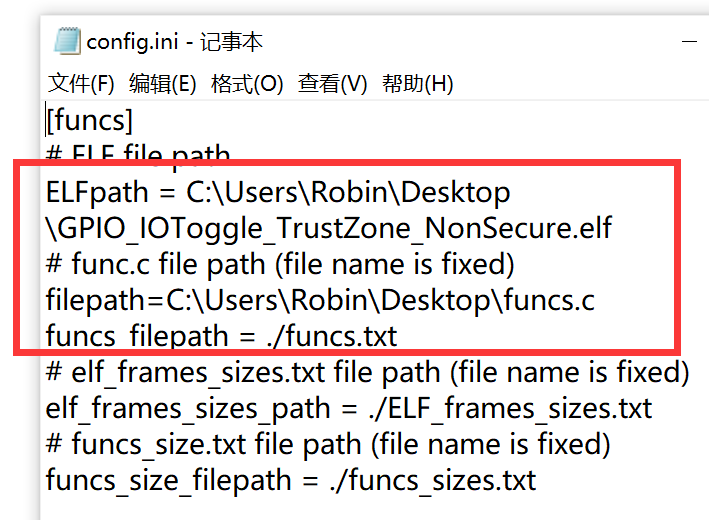
\includegraphics[scale=0.4]{graph/gailujing.png}
                        \caption{填充路径}
                        \label{gl}
                    \end{figure}
              \item 依据函数表可知修改前`func.c`共有162个函数,并且部分地址尚未改变。
                    % \begin{figure}
                    %     \centering
                    %     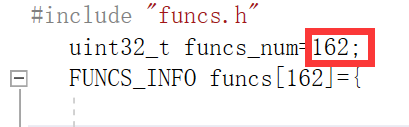
\includegraphics[scale=1]{graph/xiugaiqian1.png}
                    %     \caption{func.c修改前1}
                    %     \label{xgq1}
                    % \end{figure}
                    % \begin{figure}
                    %     \centering
                    %     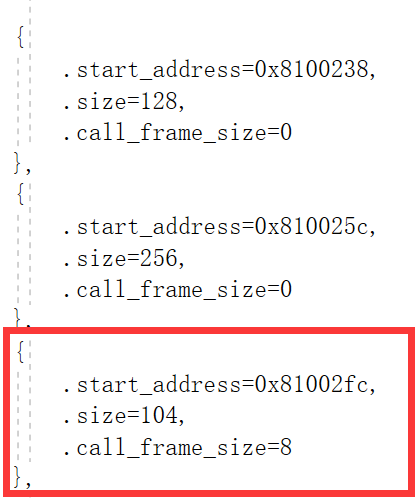
\includegraphics[scale=0.5]{graph/xiugaiqian2.png}
                    %     \caption{func.c修改前2}
                    %     \label{xgq2}
                    % \end{figure}
                    \begin{lstlisting}[language=C]{func.c修改前示例}
#include "funcs.h"
uint32_t funcs_num=@\textcolor{red}{162}@;
FUNCS_INFO funcs[@\textcolor{red}{162}@]={

{
    .start_address=0x8100238,
    .size=128,
    .call_frame_size=0
},
{
    .start_address=0x810025c,
    .size=256,
    .call_frame_size=0
},
{
    .start_address=@\textcolor{red}{0x81002fc}@,
    .size=104,
    .call_frame_size=8
},
{
    .start_address=0x8100618,
    .size=72,
    .call_frame_size=0
},} \end{lstlisting}
                    
          \end{enumerate}
    \item 终端运行
          \begin{enumerate}
              \item 运行结果如图\ref{yx}:
                    \begin{figure}[H]
                        \centering
                        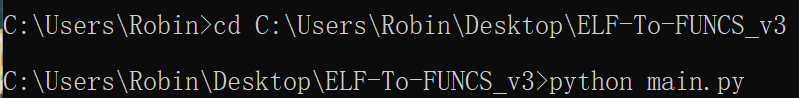
\includegraphics[scale=0.5]{graph/zhongduanjieguo.png}
                        \caption{运行结果}
                        \label{yx}
                    \end{figure}
              \item 输出函数信息以及解析数据如图\ref{sc}:
                    \begin{figure}[H]
                        \centering
                        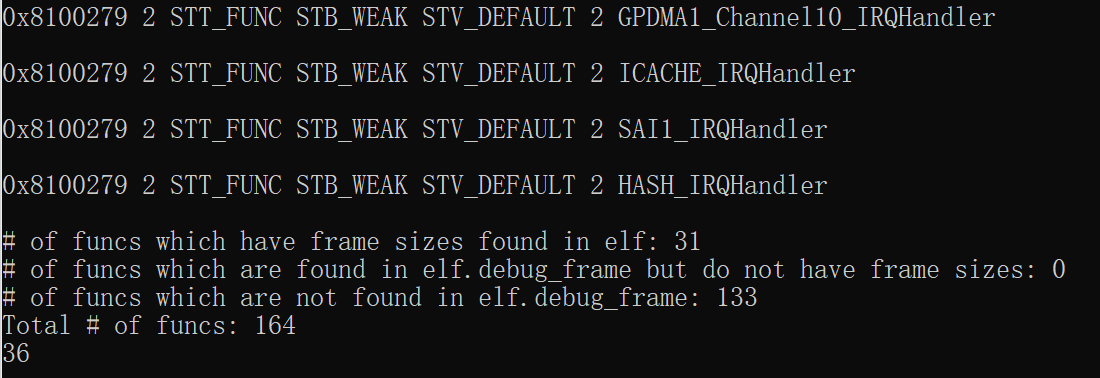
\includegraphics[scale=0.4]{graph/shuchujieguo.png}
                        \caption{输出函数信息以及解析数据}
                        \label{sc}
                    \end{figure}
              \item func.c被成功修改:
                    % \begin{figure}
                    %     \centering
                    %     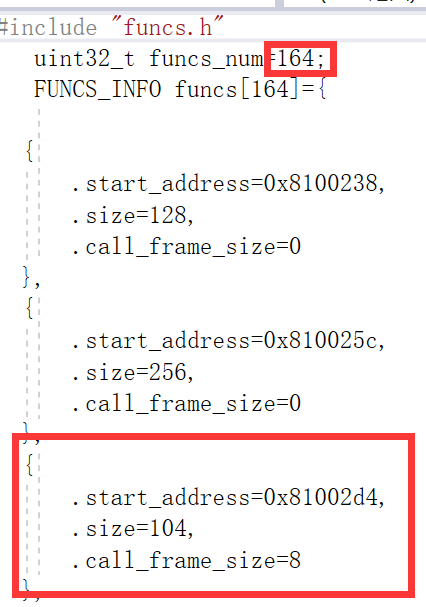
\includegraphics[scale=0.5]{graph/xiugaihou.png}
                    %     \caption{func.c修改后}
                    %     \label{xg1}
                    % \end{figure}
                    \begin{lstlisting}[language=C]{func.c修改后示例}
#include "funcs.h"
uint32_t funcs_num=@\textcolor{red}{164}@;
FUNCS_INFO funcs[@\textcolor{red}{164}@]={
    
{
    .start_address=0x8100238,
    .size=128,
    .call_frame_size=0
},
{
    .start_address=0x810025c,
    .size=256,
    .call_frame_size=0
},
{
    .start_address=@\textcolor{red}{0x81002d4}@,
    .size=104,
    .call_frame_size=8
},
{
    .start_address=0x8100618,
    .size=72,
    .call_frame_size=0
},}\end{lstlisting}
     \end{enumerate}
\end{enumerate}
\par 依据上例可见,本工具成功修改函数表,具有可行性。

\subsubsection{面向实时操作系统 FreeRTOS 的函数级地址空间布局随机化部署}
\par 本节需要在非安全世界中部署 FreeRTOS 操作系统,FreeRTOS 操作系统会在非安全世界创建任务并运行,从而触发安全世界的函数随机化安全服务,从而实现对非安全世界的函数实现地址空间随机化。
\paragraph{FreeRTOS 简介}
\par 实时操作系统(RTOS)是一种能够以足够快的速度接受并处理外界事件或数据的操作系统。它的主要特点是能够在规定的时间范围内控制生产过程或快速响应处理系统,并协调管理所有实时任务的运行。FreeRTOS是一款轻量级的开源实时操作系统,具有较小的内存占用和快速的任务切换速度,适用于资源受限的嵌入式系统。并且FreeRTOS具备良好的可移植性,可以在多种处理器架构和开发环境中使用,支持多种编译器和开发工具链。总的来说,FreeRTOS是构建高效、可靠和实时响应的嵌入式系统的理想选择。
\paragraph{FreeRTOS 在非安全世界的部署}
\begin{itemize}
    \item[(1)] 下载源码:FreeRTOS 是一款遵循 GPLv2+ 许可协议的开源免费实时操作系统。直接从 FreeRTOS 官网下载源码。下载完成后,在非安全世界下创建一个名为 FreeRTOS 的文件夹。FreeRTOS 源码包括 .c 文件(FreeRTOS 源码文件)、include 文件夹(相关头文件)、portable 文件夹(与编译器相关的文件夹,在不同的编译器中使用不同的支持文件)以及 MemMang 文件夹(与内存管理相关的文件夹)。此外,还有一个名为 FreeRTOSConfig.h 的文件,它是 FreeRTOS 的配置文件。
        
    \item[(2)] 将源码中的 .c 文件、include 文件夹和 portable 文件夹拷贝至创建的 FreeRTOS 文件夹中。在 portable 文件夹中,只保留 GCC 文件夹和 MemMang 文件夹,然后只保留 GCC 文件夹中的 ARM\_CM33 文件夹,以及 MemMang 文件夹中的 heap4.c 文件。接下来,将 Demo 文件夹下对应开发板的 FreeRTOSConfig.h 文件拷贝至作品的 include 文件夹中。
        
    \item[(3)] 配置 FreeRTOSConfig.h 文件:
        \begin{itemize}
            \item[(a)] 将 configENABLE\_TRUSTZONE 设置为 1,以支持 TrustZone 模式。
            \item[(b)] 将 configENABLE\_MPU 设置为 1,以支持内存保护单元(MPU)。
            \item[(c)] 注释掉原有作品自带的一些中断处理函数,以使用 FreeRTOS 提供的中断处理函数,例如 SysTick\_Handler、SVC\_Handler 等。
        \end{itemize}
\end{itemize}

\paragraph{对 FreeRTOS 实现函数级地址空间布局随机化}
\par 在成功将 FreeRTOS 实时操作系统部署到非安全世界后,我们需要对 FreeRTOS 实现函数级地址空间随机化。整个流程与上文所述的函数随机化流程相同,只是在对 FreeRTOS 进行函数随机化时,我们需要以下针对性的设计:
\begin{itemize}
    \item 在原有函数随机化中,我们通过 msp 栈指针获取函数的返回地址,然后对其进行随机化。然而,FreeRTOS 有 msp 和 psp 两个栈指针,其中 msp 指针用于系统内核和中断服务函数,psp 指针用于用户的任务。因此,我们需要通过 bl 寄存器的值来判断当前使用的栈指针是 msp 还是 psp,从而获取函数的返回地址。
          \begin{lstlisting}[language=C]{修改前}
initial_msp_s=__get_MSP();
secureportREAD_MSP_NS(msp); \end{lstlisting}
          \begin{lstlisting}[language=C]{修改后}
uint32_t ulLRValue;
__asm volatile("mov %0, lr" : "=r" (ulLRValue) );
if (((ulLRValue >> 3) & 1) == 0 || ((ulLRValue >> 2)&1) == 0) {
    initial_msp_s=__get_MSP();
    secureportREAD_MSP_NS_aslr(sp);
}
else {
    initial_msp_s = __get_PSP();
    secureportREAD_PSP_NS_aslr(sp);
} \end{lstlisting}
    \item FreeRTOS 中存在一些内联汇编代码,其中包含相对跳转指令 bl,这与作品的基本要求冲突。为了确保所有函数的跳转为绝对跳转,需要将 FreeRTOS 的内联汇编代码中的相对跳转指令 bl 修改为绝对跳转指令 blx。
\end{itemize}

\subsubsection{Trusted Firmware-M部署及安全服务的实现}
\paragraph{简介}
\subparagraph{QEMU简介}
\par qemu是一个开源的仿真器,可以模拟多种CPU架构,包括ARM,MIPS,x86等。在本作品中,为了研究TF-M的架构和安全服务,而不是局限于设备的复杂硬件,前期我们基于qemu模拟ARM Contex-M33内核以运行Trusted Firmware-M。
\subparagraph{调试工具GDB}
因为本作品是使用gcc-arm-none-eabi工具链编译的,所以我们使用gdb作为调试工具。qemu会在调试模式下,开启一个gdb server, 我们可以通过vscode ssh远程连接到虚拟机,并通过gdb监听本地gdb server,实现对qemu的调试。
\paragraph{自定义的安全分区}
\subparagraph{介绍}
安全服务是一种执行环境,为Root of Trust (RoT)服务提供以下功能:
\begin{itemize}
    \item 访问资源,保护其自身的代码和数据。
    \item 与系统中的其他组件进行交互的机制。
    \item 每个安全分区是执行的最小单元,并具有隔离功能。 TF-M支持添加自己的安全分区,本作品中我们添加了一个简单的安全分区,用于测试非安全区与安全区的通信。
          
\end{itemize}
\subparagraph{实现}
\par 代码组织结构
\begin{lstlisting}
example_partition
|-- CMakeLists.txt
|-- tfm_example_partition.c           //核心代码
|-- tfm_example_partition.yaml        //提供安全分区的配置信息
|-- tfm_example_partition_api.c         
|-- tfm_example_partition_api.h         
|-- tfm_example_partition_secure_api.c//安全分区的API实现

\end{lstlisting}
\par 关键代码如下:
\begin{lstlisting}[language=C]{tfm_example_partition.c}
for(int i=0;i<1;++i)
{
    psa_read(msg.handle, 0, &read_buf, msg.in_size[i]);
    LOG_INFFMT("[Example partition] Service called from client[%d]\r\n",msg.client_id);
    LOG_INFFMT("%s\r\n",read_buf);
            
    psa_crypto_init();
    psa_hash_operation_t ho=psa_hash_operation_init();
    psa_hash_setup(&ho,PSA_ALG_SHA_256);
            
    psa_status_t st = psa_hash_update(&ho,(const uint8_t *)&read_buf,msg.in_size[i]-1);
    int length=0;
    st = psa_hash_finish(&ho,write_buf,32,&length);
    if(st==PSA_SUCCESS)
    {
        LOG_INFFMT("Crypto service called successfully, sha256 for the string is:\r\n");
        for(int k=0;k<length;++k)
             LOG_INFFMT("%X",write_buf[k]);
    }
    LOG_INFFMT("\r\n");
	psa_write(msg.handle, 0, write_buf, length);
}
\end{lstlisting}
\par 基于IPC模型,安全分区可以通过$psa\_read()$函数从非安全区读取数据,然后调用$psa\_crypto\_init()$函数初始化加密服务,最后调用$psa\_hash\_finish()$函数对数据进行哈希计算,最后将计算结果通过$psa\_write()$函数写回非安全区。


\subsection{原型系统效果展示}
\subsubsection{基于QEMU模拟器的安全服务调用展示}
\par 当我们在Qemu模拟处理器上开发时,常通过终端输出字符串表示代码运行成功。
\par 例如,如图\ref{terminal},我们在Qemu模拟处理器上自定义TF-M安全服务并进行测试时(详见第二章第三小节:Trusted Firmware-M部署及安全服务的实现),终端正确输出字符串,安全服务调用成功!

\begin{figure}[H]
    \centering
    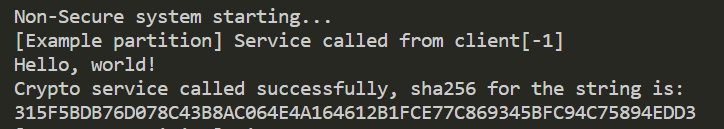
\includegraphics[scale=1.1]{graph/terminal output.png}
    \caption{Qemu模拟处理器终端输出效果}
    \label{terminal}
\end{figure}

\subsubsection{基于STM32L562E-DK开发板的系统部署展示}
\par 当我们基于STM32L562E-DK开发板进行开发工作时,常通过小灯点亮表示代码运行成功。例如,我们在部署FreeRTOS时:
\begin{itemize}
    \item[1)]首先创建任务函数,该函数接收一个小灯引脚参数,并定时给与引脚高低电平,从而使小灯点亮。小灯点亮表示FreeRTOS部署成功。关键代码如下:
    \begin{lstlisting}[language=C]{任务函数}
void vTaskLED(void * pvParameters) 
{ 
    ledInfo* info=pvParameters; 
    while(1) 
    { 
        HAL_GPIO_TogglePin(info->port, info->pin); 
        vTaskDelay(pdMS_TO_TICKS(500)); 
    } 
} \end{lstlisting}
    \item[2)]创建两个任务,并启动
    \begin{lstlisting}[language=C]{任务启动}
ledInfo redLED={LED_RED_GPIO_Port,LED_RED_Pin}; 
ledInfo greenLED={LED_GREEN_GPIO_Port,LED_GREEN_Pin}; 
// 创建点亮任务 
xTaskCreate(vTaskLED, "LED_RED", 256, &redLED, 3, NULL); 
xTaskCreate(vTaskLED, "LED_GREEN", 256, &greenLED, 3, NULL); 
// 启动任务 
vTaskStartScheduler(); \end{lstlisting}
\end{itemize}
最终,如图\ref{LightUp},成功点亮小灯,说明FreeRTOS部署成功。

\begin{figure}[htbp]
    \centering
    \begin{minipage}[t]{0.4\textwidth} %textwidth值小于0.25,或者linewidth小于0.5,不过这里设置textwidth比设置linewidth效果好一些
        \centering
        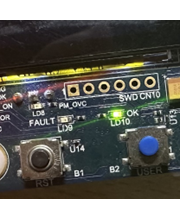
\includegraphics[scale=1]{graph/Light_up1.png}
    \end{minipage}
    \hspace{0.3in} % 两图片之间的距离
    \begin{minipage}[t]{0.4\textwidth}%textwidth值小于0.25
        \centering
        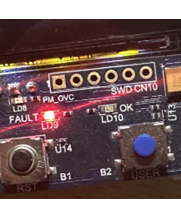
\includegraphics[scale=1]{graph/Light_up2.png}
    \end{minipage}
    \caption{小灯点亮}
    \label{LightUp}
\end{figure}

\subsubsection{FASLR动态实时函数网页展示平台}
\par 为了更清晰的显示函数在内存上的位置变化以及FASLR的工作流程,我们对函数在内存中的位置进行实时获取,并通过如图\ref{web}所示的网页端进行展示。我们将Flash内存中的函数显示至左侧的表格中,并根据函数的调用情况,借助MPU对其进行随机化,实时展示其随机化后的位置(RAM内存),并展示在右侧的表格中。

\begin{figure}[H]
    \centering
    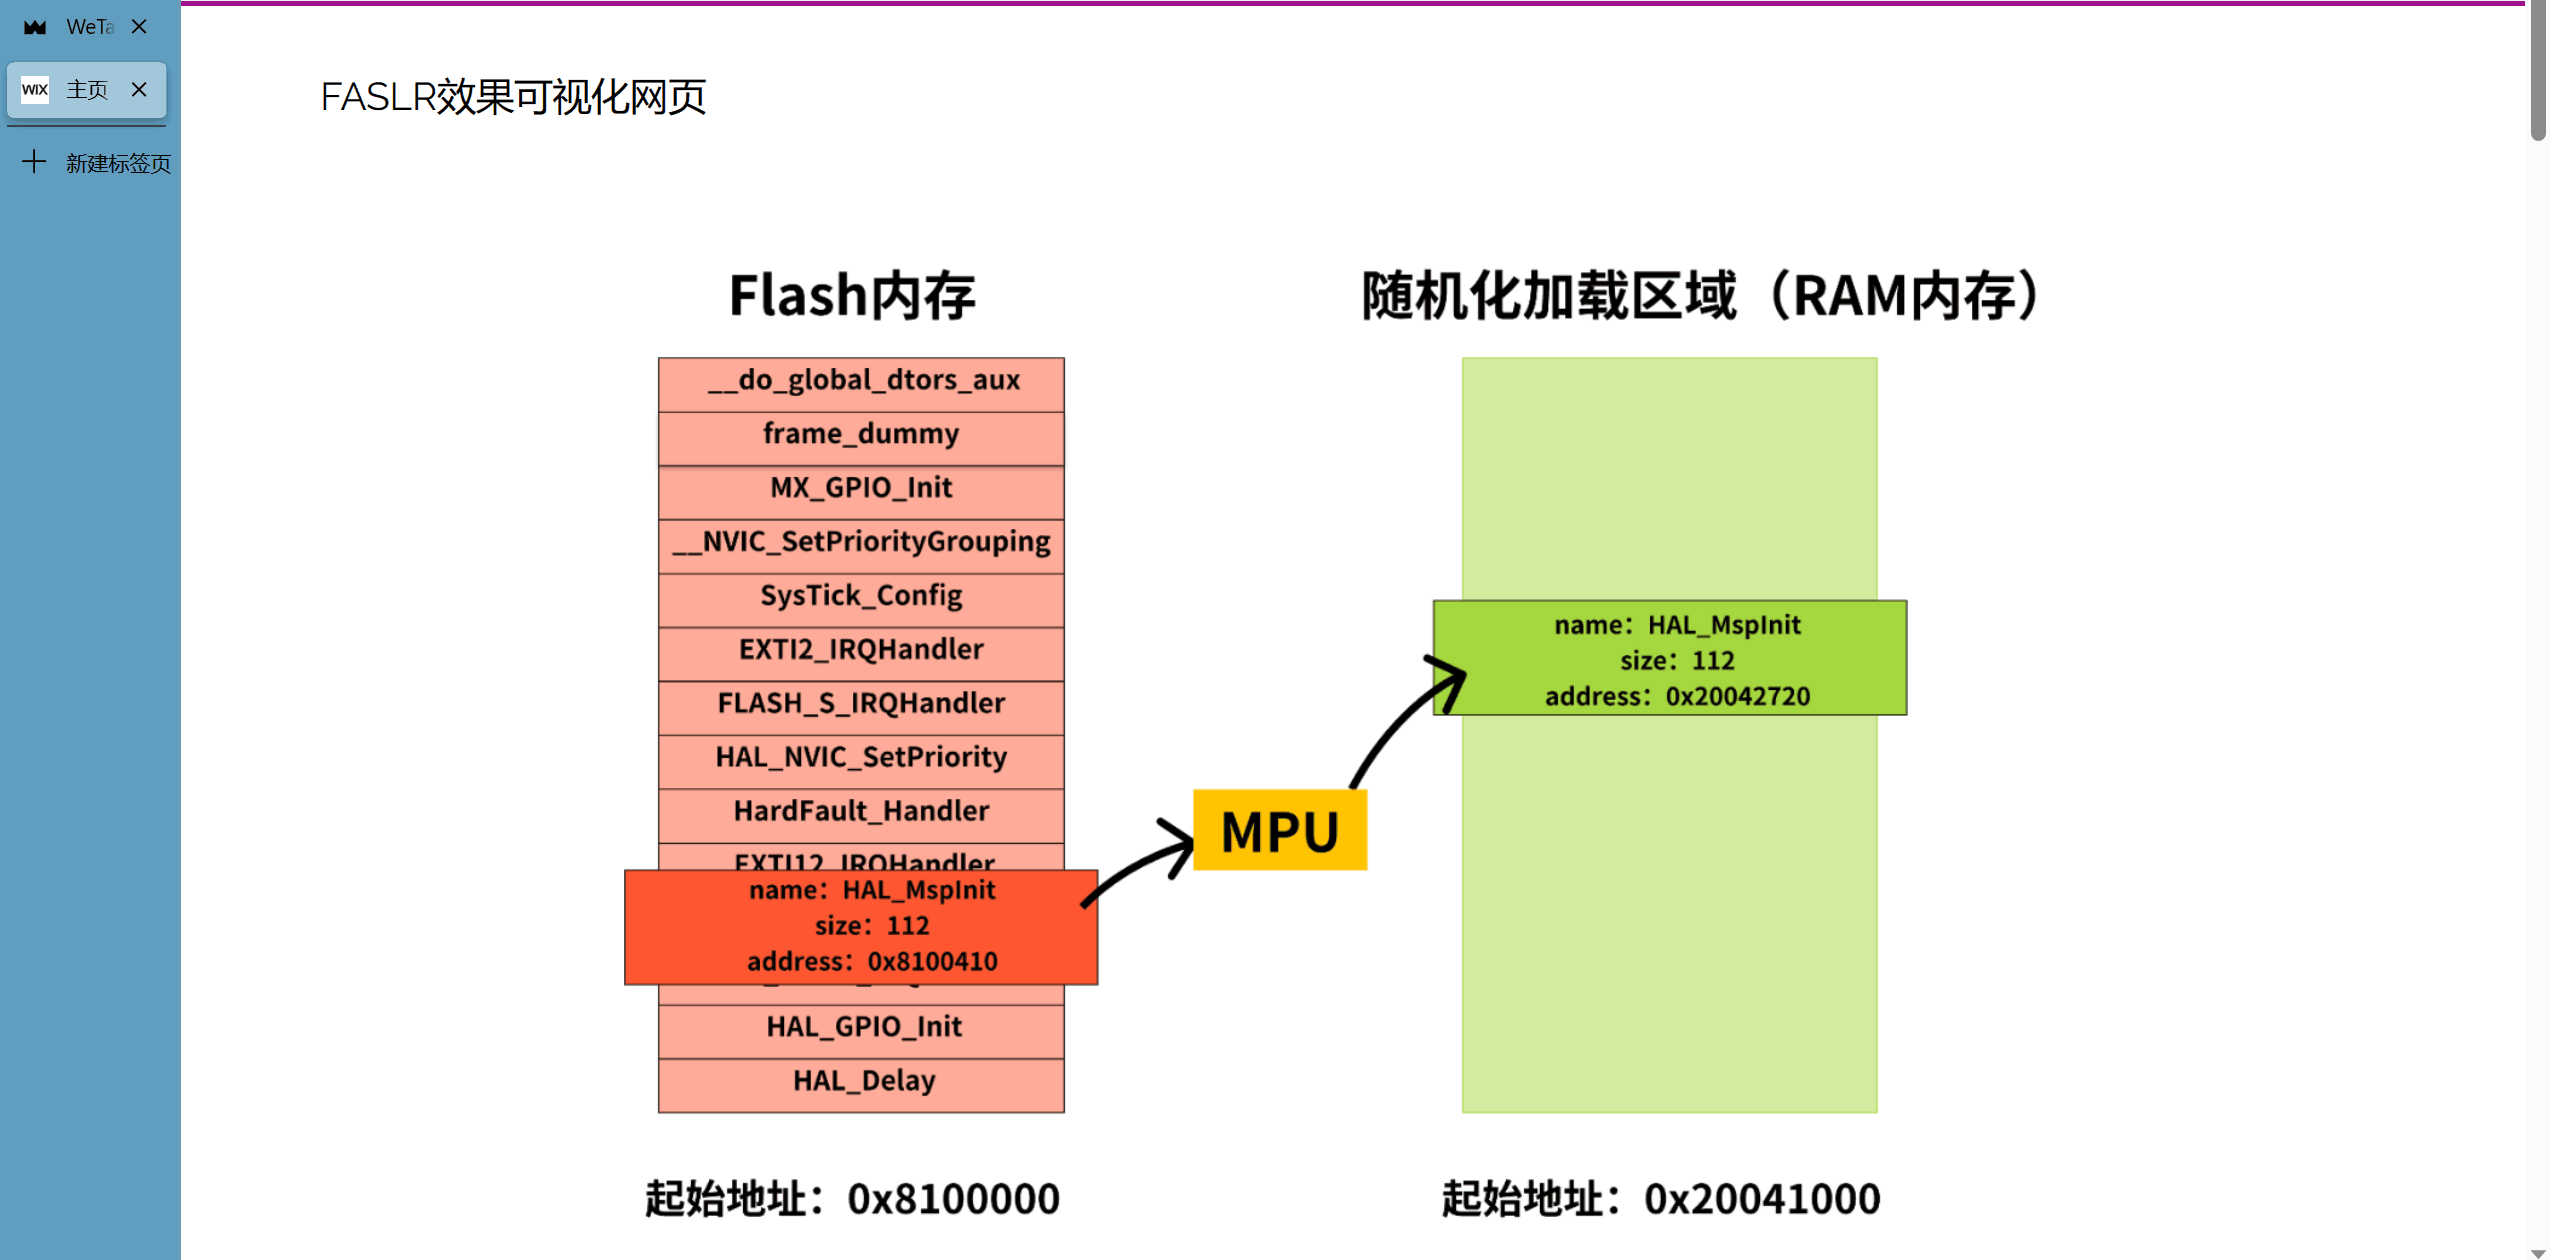
\includegraphics[scale=0.15]{graph/web1.png}
    % \caption{FASLR可视化网页界面}
    %\label{web1}
\end{figure}
\begin{figure}[H]
    \centering
    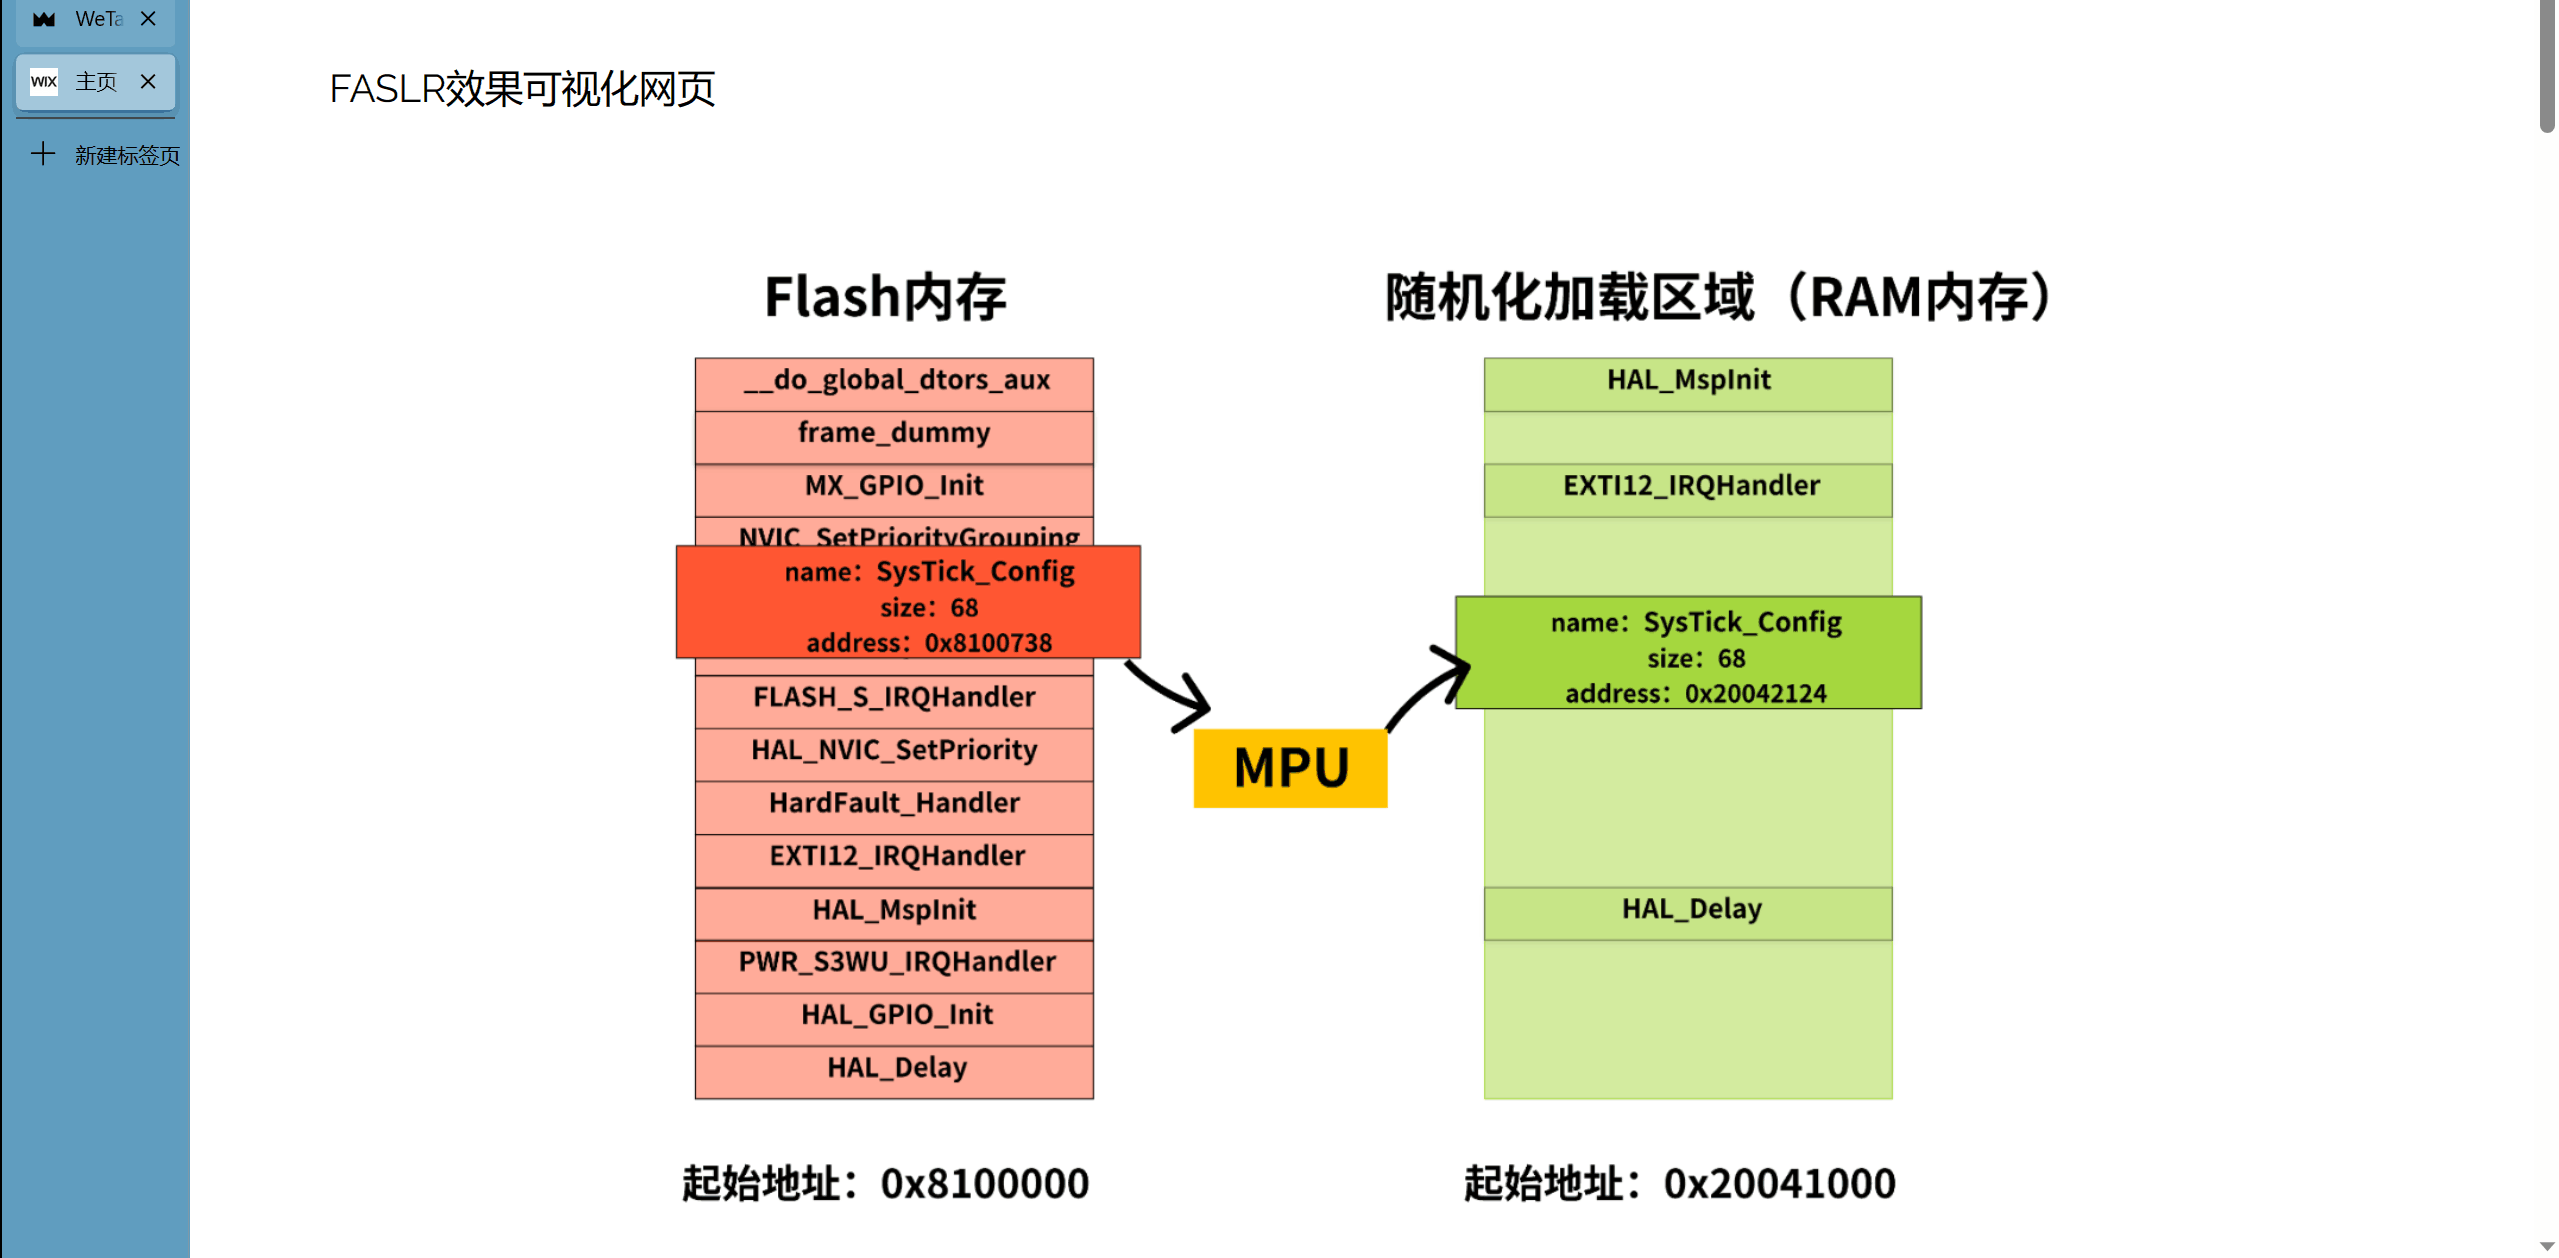
\includegraphics[scale=0.15]{graph/web2.png}
    \caption{FASLR可视化网页界面}
    \label{web}
\end{figure}


\section{作品测试与分析}
\subsection{测试环境}
\begin{itemize}
    \item[1)] 硬件环境:SAML11 Xplained Pro 开发板一块,STM32L562 开发板一块;
    \item[2)] 软件环境: Qemu 模拟处理器;
    \item[3)] 开发工具:STM32CubeIDE、VS Code;
    \item[4)] 开发语言:C/C++、ARM Assemble、python、shell。
\end{itemize}
\subsection{测试方案}
\subsubsection{安全性测试与分析}
\paragraph{威胁模型}
\par 假设攻击者只能在程序运行期间实行攻击。本作品不考虑对于固件的离线攻击,比如对固件的重写,对总线的监听或者内存的篡改等等。本作品认为攻击者具有利用整个非安全世界漏洞以及安全世界非特权漏洞的能力,最终可以实现对内存的任意读写,包括代码段,数据段,堆和栈,以及非安全世界的系统配置资源,只有安全世界的内核(运行于特权态)是可信的。本作品默认安全模块(Secure Module)运行在安全世界的非特权状态。
\paragraph{安全性原理分析}
\par 假设该物联网设备有身份认证功能,用户需要输入密码后才能启动该设备,攻击者将基于以下三种技术劫持控制流,绕过身份认证功能,直接进入系统。
\par 攻击者利用代码注入攻击,直接将想要执行的函数写入栈中后,将程序流寄存器R15 劫持到栈上执行相应语句,因为在程序启动时 MPU 将会默认对栈分配不可执行的权限,所以攻击者只能注入恶意代码而无法执行恶意代码。
\par 攻击者因为不可执行的保护措施无法直接运行注入的代码,但可以基于 ROP 攻击利用程序中已有的代码。攻击者将函数返回时的栈帧中的返回地址覆盖为程序中gadgets 组合的地址,以执行攻击者预想的程序流,而在 Flash 空间(代码段固定,gadgets 地址已知)中关键的 gadgets 已经被 MPU 禁止执行,RAM 空间(代码段地址随机分布)中的 gadgets 地址无法获取,达到阻断 ROP 攻击链的目的,其中 ROP 链如图\ref{ROP blocking process}所示。
\begin{figure}[H]
    \centering
    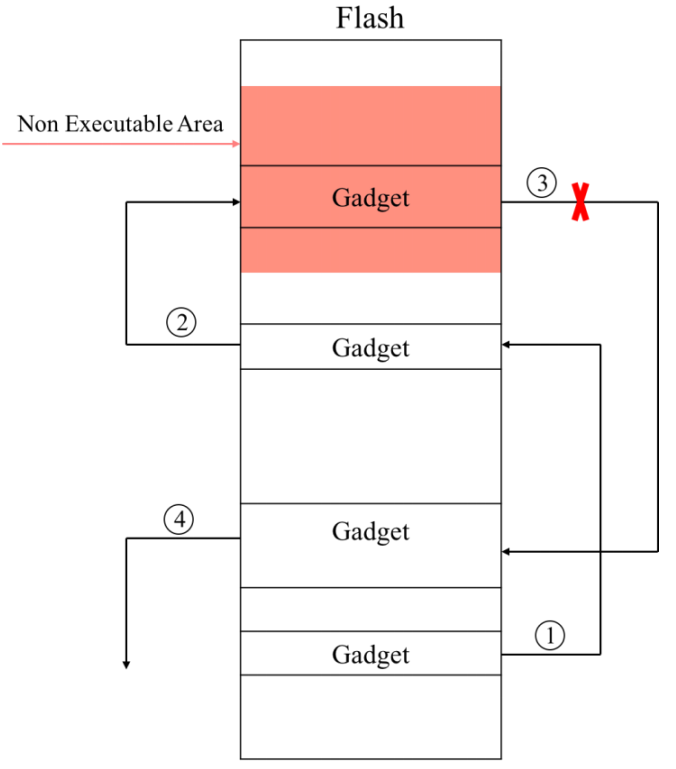
\includegraphics[scale=0.55]{graph/ROP blocking process.png}
    \caption{ROP链阻断流程}
    \label{ROP blocking process}
\end{figure}
\par 攻击者无法利用完整 ROP 链中的 gadgets,但可以对位于 RAM 空间中 gadgets 的地址进行暴力求解。猜测只能是一次性的,若猜测错误,ROP 链则会断裂,程序执行流无法被劫持,而猜测一次成功的概率仅有 1/16KB。

\subsubsection{性能与内存开销测试}
\par 为了说明FASLR的可用性以及低开销,本作品将FASLR在Microchip 的SAML11 Xplained Pro开发板上进行部署并对其进行运行时性能、内存以及运行时随机熵分布的实验评估。SAML11是一款基于ARM Cortex-M23处理核心并搭载有TrustZone-M的SoC,它配备有64KB的Flash内存以及16KB的RAM内存。本作品使用GNU Arm Embedded Toolchain对FASLR以及非安全世界的应用程序进行编译,其中,为了使非安全世界应用程序的代码中没有使用相对寻址模式的函数调用,编译时使用了两个额外的编译标志:-mlong-calls和-fno-jump-tables,同样的,本作品对编译所用到的C库也用上述编译标志进行编译。在编译过程中,本作品使用一个Python函数自动化提取工具对编译得到的ELF文件进行函数信息的提取,并将其保存在Function Table中。FASLR将安全应用程序以及Function Table部署在安全世界Flash内存中,用户的应用程序被部署在非安全世界的Flash内存中。
\par 本作品将FASLR部署在21个应用程序上并对其进行运行时性能开销、内存开销以及运行时随机熵分布的评估。其中包括一个自主研发的空气质量监测系统以及一些嵌入式领域公开的示例程序。空气质量检测系统的实物图如图\ref{physicalDrawing}所示,它包括一个SAML11开发板、空气质量检测模块PMSA003、蜂窝模块SIM7000以及电源供给模块。非安全世界的应用程序会周期性的从PMSA003获取PM2.5的数据并将该数据通过SIM7000C以MQTT协议发送至AWS IoT平台。另外二十个应用程序包括一个CoreMark Benchmark\cite{CoreMarkBenchmark}、两个Microcontroller Benchmark Cache Test和Matrix Multiply、九个BEEBS Benchmark\cite{BEEBSBenchmark}的应用程序以及Atmel官方\cite{Atmel}提供的针对SAML11的示例程序。
\begin{figure}[H] %\cite{Matrix}、
    \label{physicalDrawing}
    \centering
    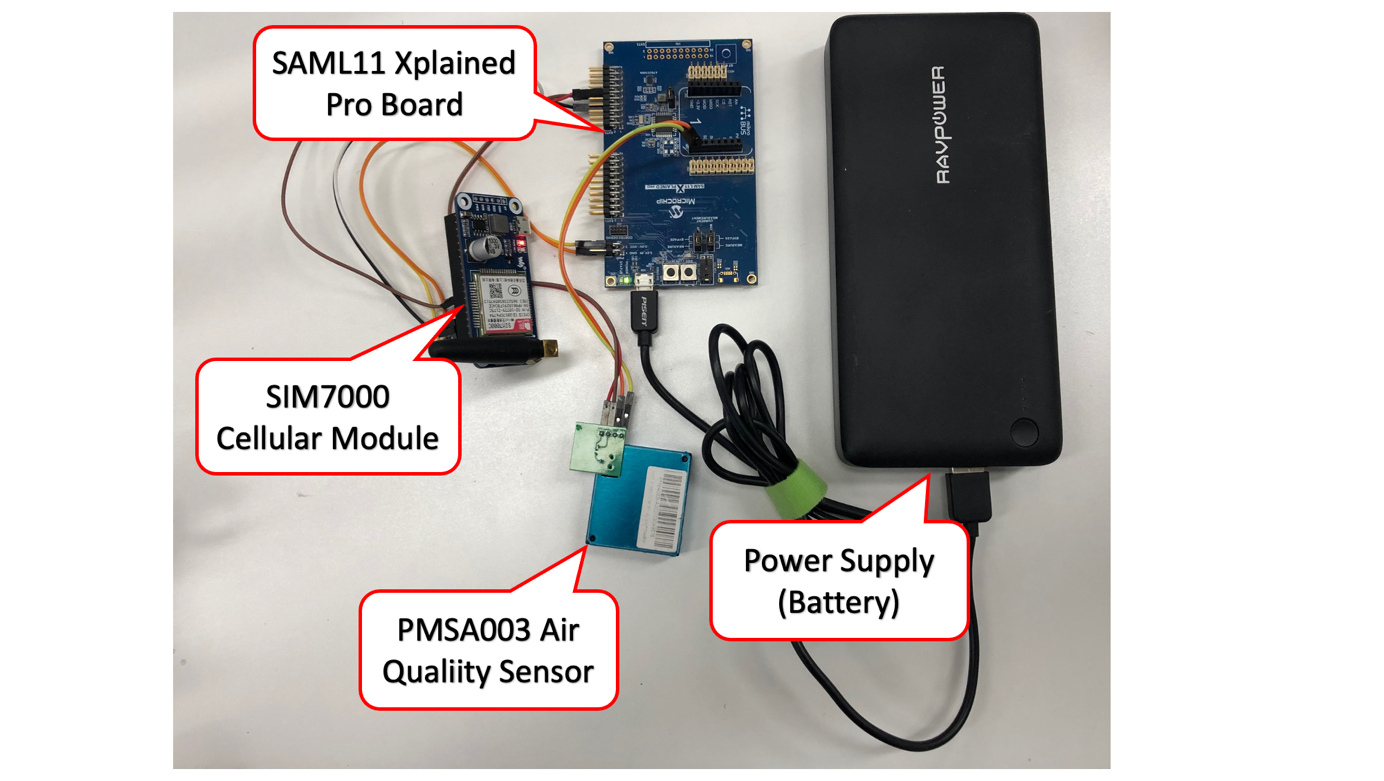
\includegraphics[scale=0.8]{graph/physicalDrawing.png}
    \caption{空气质量监测系统实物图}
\end{figure}

\subsection{测试数据及分析}

\subparagraph{性能评估}
\par FASLR所引入的性能开销主要是因为非安全世界应用程序对Flash上的函数调用时,FRE对该函数执行随机化将会产生额外的运行时间。本作品对上述21个应用程序在部署FASLR的情况下的运行时间进行记录,并将其与未部署FASLR的情况下的运行时间进行对比。本作品使用ARM处理器核心提供的SysTick定时器以记录程序的运行时间,精确度为0.01秒。由于物联网应用程序大多为一个循环程序,因此,本作品为每一个应用程序设置固定循环次数以测试其运行时性能开销。测试结果如表\ref{table1}所示,可以发现FASLR的性能开销不超过10\%,并且有14个应用程序的性能开销小于5\%。此外,本作品对函数内存回收的次数进行了统计,结果表示,19个应用程序由于RAM内存限制而进行了至少一次的函数内存回收。
\begin{longtable}{ccccc}
    % \centering  % 显示位置为中间
    \caption{FASLR性能测试结果}  % 表格标题
    \label{table1}                                            \\ % 用于索引表格的标签
    % \begin{tabular}{ccccc}
    \hline
    应用程序                 & 清理次数 & 基准时间    & FASLR   & 性能开销    \\ \hline
    AirqualityMonitor    & 1    & 324.79s & 327.50s & 0.83\%  \\ 
    Coremark             & 4    & 15.62s  & 15.78s  & 1.02\%  \\ 
    Cache Test           & 2    & 2.13s   & 2.26s   & 6.10\%  \\ 
    Matrix Multiply      & 1    & 24.47s  & 26.13s  & 6.78\%  \\ 
    SecureDriver         & 1    & 12.56s  & 12.64s  & 0.64\%  \\ 
    ADC Event System     & 2    & 12.41s  & 12.54s  & 1.04\%  \\ 
    Calendar             & 0    & 50.36s  & 50.33s  & -0.06\% \\ 
    Light Sensor         & 1    & 24.77   & 25.36s  & 2.38\%  \\ 
    Low Power for SAML1X & 0    & 14.60s  & 14.60s  & 0\%     \\ 
    ADP Hello            & 1    & 9.93s   & 10.88s  & 9.57\%  \\ 
    SAML11-CRYA          & 1    & 6.79s   & 7.35s   & 8.25\%  \\ 
    SAML11-TrustRAM      & 1    & 1.14s   & 1.25s   & 9.65\%  \\ 
    Beebs-crc            & 1    & 7.44s   & 7.73s   & 3.90\%  \\ 
    Beebs-aha-mont64     & 1    & 7.30s   & 7.73s   & 3.56\%  \\ 
    Beebs-aha-compress   & 1    & 4.50s   & 4.67s   & 3.78\%  \\ 
    Beebs-bs             & 1    & 0.28s   & 0.29s   & 3.57\%  \\ 
    Beebs-bubblesort     & 1    & 0.33s   & 0.35s   & 6.06\%  \\ 
    Beebs-compress       & 2    & 2.02s   & 2.18s   & 7.92\%  \\ 
    Beebs-md5            & 2    & 0.42s   & 0.44s   & 4.76\%  \\ 
    Beebs-levenshiein    & 1    & 17.42s  & 17.97s  & 3.16\%  \\ 
    Beebs-edn            & 2    & 15.96s  & 16.24s  & 1.75\%  \\ \hline
    % \end{tabular}
\end{longtable}

\subparagraph{内存评估}
\par 为评估FASLR的内存开销,本作品对每个应用程序总共的函数数量以及部署FASLR前后应用程序所占内存空间大小(包括代码大小以及静态数据大小)进行对比,应用程序所占内存空间大小的变化主要来源于编译阶段的两个特殊的编译选项,其内存开销结果如表\ref{table2}所示,可以发现21个应用程序的内存开销都小于5\%。
\begin{longtable}{ccccc}
    % \centering  % 显示位置为中间
    \caption{FASLR内存资源测试结果}
    \label{table2}                                         \\
    \hline
    应用程序                 & 总函数个数 & 基准内存大小 & FASLR & 内存开销   \\ \hline
    AirqualityMonitor    & 148   & 41092  & 43036 & 4.73\% \\ 
    Coremark             & 174   & 46048  & 47648 & 3.47\% \\ 
    Cache Test           & 140   & 40228  & 41844 & 4.02\% \\ 
    Matrix Multiply      & 145   & 40728  & 42404 & 4.12\% \\ 
    SecureDriver         & 139   & 39544  & 41184 & 4.15\% \\ 
    ADC Event System     & 173   & 43036  & 44640 & 3.73\% \\ 
    Calendar             & 97    & 36780  & 36808 & 0.08\% \\ 
    Light Sensor         & 132   & 40496  & 40528 & 0.08\% \\ 
    Low Power for SAML1X & 67    & 34136  & 34164 & 0.08\% \\ 
    ADP Hello            & 99    & 38072  & 38316 & 0.64\% \\ 
    SAML11-CRYA          & 143   & 41368  & 43012 & 3.97\% \\ 
    SAML11-TrustRAM      & 142   & 39896  & 41500 & 4.02\% \\ 
    Beebs-crc            & 138   & 39944  & 41492 & 3.88\% \\ 
    Beebs-aha-mont64     & 142   & 40476  & 42028 & 3.83\% \\ 
    Beebs-aha-compress   & 140   & 39944  & 41492 & 3.88\% \\ 
    Beebs-bs             & 137   & 39344  & 40896 & 3.94\% \\ 
    Beebs-bubblesort     & 137   & 39932  & 40892 & 2.40\% \\ 
    Beebs-compress       & 143   & 40808  & 42360 & 3.80\% \\ 
    Beebs-md5            & 137   & 41552  & 43100 & 3.73\% \\ 
    Beebs-levenshiein    & 138   & 39708  & 41348 & 4.13\% \\ 
    Beebs-edn            & 144   & 42112  & 43736 & 3.86\% \\ \hline
\end{longtable}

\subparagraph{运行时随机熵分布评估}
\par 由于攻击者可能使用暴力破解攻击以绕过FASLR并实行代码复用攻击,FASLR通过一下两种方式以抵御暴力破解攻击:(1)FASLR通过对Flash内存上的函数设置不可执行,保证只有在随机加载区域的函数可以执行,从而限制了运行时可以被代码复用的函数数量。(2)即使攻击者能在随机加载区域的函数中找到代码复用攻击所需要所有gadgets,攻击者必须需要一次猜对所有gadgets所在的位置。公式(4)给出了随机加载区域的所有可能的函数布局数量。其中k表示随机加载区域内已加载的函数个数,V为随机加载区域剩余的内存空间大小的一半(ARMv8-M架构下只允许函数入口地址为偶数),随机加载区域剩余内存空间可以被表示为V个空闲单元,每个空闲单元为2字节,若随机加载区域剩余内存大小为64KB,则V为32K。
\begin{equation}
    C = k!\tbinom{V+k}{k}
\end{equation}
\par 本作品假设随机加载区域剩余内存空间足够放置k个函数,如果所有的剩余空闲块都不足以加载当前函数,则可以执行块合并操作以消除块管理机制导致的内存碎片化。攻击者需要面对的是在保证剩余空间为V个空闲单元的情况下插入k个函数所有可能的组合情况,该组合个数可以通过二项式系数$\tbinom{V+k}{k}$与k!相乘获得,k!表示k个函数都不相同。举例来说,如果k=5且V=100,那么其总的组合个数为:
\begin{equation}
    5!\tbinom{100+5}{5}=1.159e+10
\end{equation}
\par 函数在随机加载区域的布局概率与C互为倒数,即概率P=1/C,公式(6)给出了随机化过程中的随机熵H。
\begin{equation}
    H=-\sum_{i=1}^C P\log_2 P = -\sum_{i=1}^{C} \frac{1}{C}\log_2 \frac{1}{C} = \log_2 C
\end{equation}
\par 在实验测试过程中,由于函数随机记载区域的剩余空间大小以及已加载函数的个数随着程序的运行而动态变化,本作品对每一个测试程序随机熵的变化进行跟踪并用箱线图对其进行记录,程序的序号与表4 1中程序的顺序相对应。图\ref{randomEntropy}展示了21个应用程序对应的运行时随机熵分布,从结果可以看到最小的平均随机熵为80左右,对于暴力破解攻击来说该解空间依旧十分巨大。
\begin{figure}[H]
    \label{randomEntropy}
    \centering
    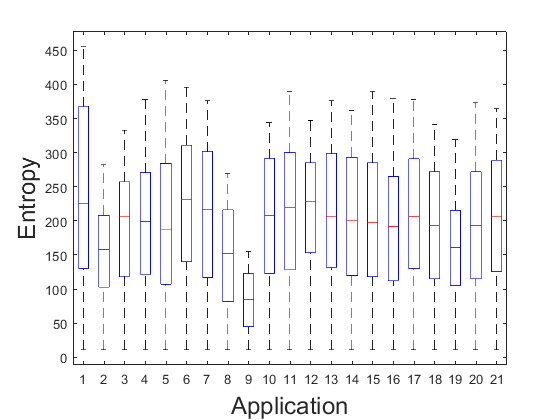
\includegraphics[scale=0.7]{graph/randomEntropy.png}
    \caption{21个应用程序的随机熵分布图}
\end{figure}

\section{创新性说明}
\subsection{面向实时操作系统以及可信执行环境实现的函数级动态地址空间布局随机化技术}
\par 在嵌入式系统领域,可信执行环境(Trusted Execution Environment,TEE)和实时操作系统(Real-Time Operating System,RTOS)都是非常重要的概念。可信执行环境是一种安全技术,可以保护程序在执行过程中的数据和代码不被篡改和窃取,是一种非常重要的硬件安全技术。而实时操作系统则是嵌入式系统中的核心组成部分,它可以保证系统对于外部事件的响应时间具有确定性,从而满足实时性的需求。

\par FreeRTOS是一款开源的、可裁剪的、轻量级的实时操作系统。它针对微处理器和微控制器设计,可以在资源受限的环境中高效运行。由于其开源和轻量级的特点,FreeRTOS在嵌入式系统领域得到了广泛的应用。

\par Trusted Firmware(TF-M)是一款开源的、针对Arm Cortex-M系列微控制器的可信执行环境框架。TF-M利用了Arm的TrustZone-M技术,实现了一种硬件隔离的安全架构,可以为嵌入式设备提供一套全面的安全解决方案。

\par 在本作品中,我们针对FreeRTOS和TF-M设计了一种基于TrustZone-M的函数级地址空间布局随机化(ASLR)技术。ASLR是一种安全防御技术,通过在每次程序启动时,随机化函数的地址布局,使得攻击者无法预测到函数的实际运行地址,从而阻止了如Return Oriented Programming(ROP)这类代码复用攻击。ROP攻击是一种常见的缓冲区溢出攻击手法,通过复用程序中已有的代码片段,可以绕过执行防护,执行任意代码。

\subsection{计算和内存资源受限场景下的高性能高利用率的随机化技术}
\par 嵌入式系统由于其特殊的应用场景和硬件环境,使得其在实现高效和安全的同时,面临着许多挑战。函数运行时的语义信息弱,状态难以感知,函数的栈帧大小不一,这些都给函数的管理和保护带来了困难。同时,函数的入口地址往往难以动态地进行修改,调用关系复杂,这些都使得函数容易成为ROP攻击的目标。此外,低端嵌入式系统的RAM资源有限,如果直接采用传统的地址空间布局随机化(ASLR)技术,可能会导致性能开销过大。

\par 针对这些挑战,我们设计了一种高效的静态信息提取机制。通过在程序的编译阶段,收集函数的信息,如函数的大小,调用关系等,并将这些信息存储起来,用于运行时的管理和调度。这样,我们就可以实现对函数运行时状态的实时感知。

\par 同时,我们设计了一种基于内存保护单元(MPU)的函数动态加载机制。通过在每次函数调用时,利用MPU设置新的函数地址,我们可以实现对函数地址空间布局的实时随机化,隐藏函数的实际运行地址,从而阻止ROP等攻击。

\par 最后,我们还设计了一种函数级随机化内存管理机制。通过在每次函数加载时,根据函数的大小和当前内存的使用情况,动态地分配内存空间,我们可以实现高利用率、高性能的内存管理,从而降低了函数级ASLR的性能开销。

\par 通过这三个机制的结合,我们的作品可以在资源有限的嵌入式设备中,实现高效、高性能的函数级ASLR,提高了设备的安全性能,抵御了ROP等攻击。同时,由于这些机制的设计都充分考虑了嵌入式设备的特性,使得我们的作品具有较好的可用性和实用性


\section{总结}
\subsection{可信执行环境TF-M}
\par 本作品以 Trusted Firmware-M 为基础框架,首先,详细的对TF-M的系统架构做了介绍,TF-M 旨在提供一个可配置和可裁剪的安全固件平台,以支持从小型嵌入式设备到高端安全系统的多种应用场景。之后,我们对TF-M做了低端的研究,在QEMU虚拟机中测试,首先移植了Trusted Firmware-M,并向其添加自定义的安全服务并对其进行调试。
\subsection{函数级地址空间布局随机化}
\par 本作品使用一种基于MPU的函数级地址空间布局随机化技术ASLR。首先,给出了系统假设以及威胁模型。其次,介绍了ASLR的设计目标及其系统方案。具体工作包括:1)为对函数信息进行收集管理,设计静态信息提取机制;2)为防止代码复用并对函数实现动态劫持,设计基于MPU的系统安全启动机制;3)为对函数进行动态随机化加载,设计函数级随机化加载机制。随后,针对随机化过程中内存受限问题,具体设计了:1)碎片化内存随机管理机制,通过显式空闲块链表结构对内存进行分配与回收,实现对碎片化内存的高效管理;2)基于调用栈展开的函数完成识别机制,通过函数栈帧中的返回信息,实现系统运行时函数返回的动态识别;3)基于函数级缓存的内存回收机制,通过函数调用重定向以及函数按需回收方法,实现对随机加载区域中函数内存的高利用率。最后,我们在原型系统中对其进行了性能测试。
\subsection{开源实时操作系统FreeRTOS}
\par 本作品在非安全世界中引入开源实时操作系统FreeRTOS,FreeRTOS 是一款轻量级的开源实时操作系统,具有较小的内存占用和快速的任务切换速度,适用于资源受限的嵌入式系统。在移植FreeRTOS在特定的嵌入式设备之后,我们又将函数级地址空间布局随机化运用在FreeRTOS中,实现了非安全区任务调度的随机化。
\clearpage
\pagestyle{refStyle}
\addcontentsline{toc}{section}{参考文献}
\bibliographystyle{unsrt}
\bibliography{ref}
\end{document}